\PassOptionsToPackage{unicode}{hyperref}
\PassOptionsToPackage{hyphens}{url}
\documentclass[
]{article}
\usepackage{xcolor}
\usepackage{amsmath,amssymb}
\usepackage{graphicx}
\setcounter{secnumdepth}{-\maxdimen} % remove section numbering
\usepackage{iftex}
\ifPDFTeX
  \usepackage[T1]{fontenc}
  \usepackage[utf8]{inputenc}
  \usepackage{textcomp} % provide euro and other symbols
\else % if luatex or xetex
  \usepackage{unicode-math} % this also loads fontspec
  \defaultfontfeatures{Scale=MatchLowercase}
  \defaultfontfeatures[\rmfamily]{Ligatures=TeX,Scale=1}
\fi
\usepackage{lmodern}
\ifPDFTeX\else
  % xetex/luatex font selection
\fi
% Use upquote if available, for straight quotes in verbatim environments
\IfFileExists{upquote.sty}{\usepackage{upquote}}{}
\IfFileExists{microtype.sty}{% use microtype if available
  \usepackage[]{microtype}
  \UseMicrotypeSet[protrusion]{basicmath} % disable protrusion for tt fonts
}{}
\makeatletter
\@ifundefined{KOMAClassName}{% if non-KOMA class
  \IfFileExists{parskip.sty}{%
    \usepackage{parskip}
  }{% else
    \setlength{\parindent}{0pt}
    \setlength{\parskip}{6pt plus 2pt minus 1pt}}
}{% if KOMA class
\KOMAoptions{parskip=half}}
\makeatother
\usepackage{longtable,booktabs,array}
\newcounter{none} % for unnumbered tables
\usepackage{calc} % for calculating minipage widths
% Correct order of tables after \paragraph or \subparagraph
\usepackage{etoolbox}
\makeatletter
\patchcmd
\longtable{\par}{\if@noskipsec\mbox{}\fi\par}{}{}
\makeatother
% Allow footnotes in longtable head/foot
\IfFileExists{footnotehyper.sty}{\usepackage{footnotehyper}}{\usepackage{footnote}}
\makesavenoteenv{longtable}
\setlength{\emergencystretch}{3em} % prevent overfull lines
\providecommand{\tightlist}{%
  \setlength{\itemsep}{0pt}\setlength{\parskip}{0pt}}
\usepackage{bookmark}
\IfFileExists{xurl.sty}{\usepackage{xurl}}{} % add URL line breaks if available
\urlstyle{same}
\hypersetup{
  hidelinks,
  pdfcreator={LaTeX via pandoc}}
\author{}
\date{}
\usepackage[
    left=2.5cm,
    right=2.5cm,
    top=3cm,
    bottom=3cm
]{geometry}
\usepackage{wrapfig}

\begin{document}

\section{\texorpdfstring{\textbf{Abstract}}{Abstract}}\label{abstract}

Operational air quality forecasts are becoming increasingly relevant for
public health and environmental decision-making. In Chile, such
decision-making is currently supported by SINCA (National Air Quality
Information System), which is based on an air quality monitoring network
and meteorological forecasts.

Operational air quality prediction in complex urban regions represents a
scientific challenge due to the strong dependence of pollutant
concentrations on meteorological conditions, topography, and the
temporal variability of emissions. In Central Chile, major air pollution
episodes are modulated by atmospheric stability processes, coastal
ventilation, and topographic confinement, requiring forecasting systems
capable of accurately representing the spatial and temporal evolution of
atmospheric pollutants.

In this study, we evaluate the capability of a coupled WRF--CHIMERE
system to reproduce and forecast the spatiotemporal variability of
atmospheric pollutants over Central Chile. To this end, multiple
meteorological and chemical simulations were performed using different
physical parameterizations, spatial resolutions, and emission
inventories. Model performance was assessed through statistical metrics
and comparisons against surface observations. The analysis considered
both the temporal representation of critical pollution episodes and the
spatial distribution of pollutant concentrations under different
meteorological regimes.

\section{\texorpdfstring{\textbf{Introduction}}{Introduction}}\label{introduction}

\section{\texorpdfstring{\textbf{General
Objective}}{General Objective}}\label{general-objective}

To develop and evaluate an operational air quality forecasting system
based on the coupling of WRF and CHIMERE for Central Chile, with
emphasis on its ability to reproduce and anticipate the spatial and
temporal variability of atmospheric pollutants.

\section{\texorpdfstring{\textbf{Specific
Objectives}}{Specific Objectives}}\label{specific-objectives}

\begin{enumerate}
\def\labelenumi{\arabic{enumi}.}
\tightlist
\item  Evaluate the meteorological performance of the WRF model using
  multiple physical parameterizations and spatial resolutions,
  considering key variables governing pollutant transport and
  dispersion, including wind,temperature, atmospheric stability and
  planetary boundary layer height, in order to select the most
  appropriate configurations for its coupling with the CHIMERE transport
  model in order to establish an operational air quality forecast system
  over Central Chile.\\
\item  Assess the capability of the WRF--CHIMERE system to represent the
  temporal and spatial variability of atmospheric pollutants (PM25,
  PM10, CO, and NOx), including the diurnal cycle, high-concentration
  episodes, temporal persistence, phase errors, forecast window
  evolution, topographic effects, accumulation and ventilation zones and
  regional transport patterns.
\end{enumerate}

\section{\texorpdfstring{\textbf{Methodology}}{Methodology}}\label{methodology}

\subsection{\texorpdfstring{\textbf{Meteorological System
Configuration}}{Meteorological System Configuration}}\label{meteorological-system-configuration}

The WRF meteorological model was implemented using multiple physical
parameterizations and spatial resolutions designed to adequately
represent the meteorological conditions of Central Chile, which are
characterized by complex topography, land-sea breezes, and seasonal synoptic variability. In particular, the Santiago basin is characterized for its prevailing southwestern summer winds, with a higher frequency of calm, stable days in winter leading to high pollution events.

A forecasting framework was adopted consisting of a 10-day spin-up
period followed by ten consecutive daily forecasts during the 2021
winter season. Each of these daily forecasts have a length of 144 hours,
for which we derive 4 lead times to consider in the analysis, as represented in the scheme of the Figure 1.

\begin{wrapfigure}{r}{0.40\textwidth}
	\centering
	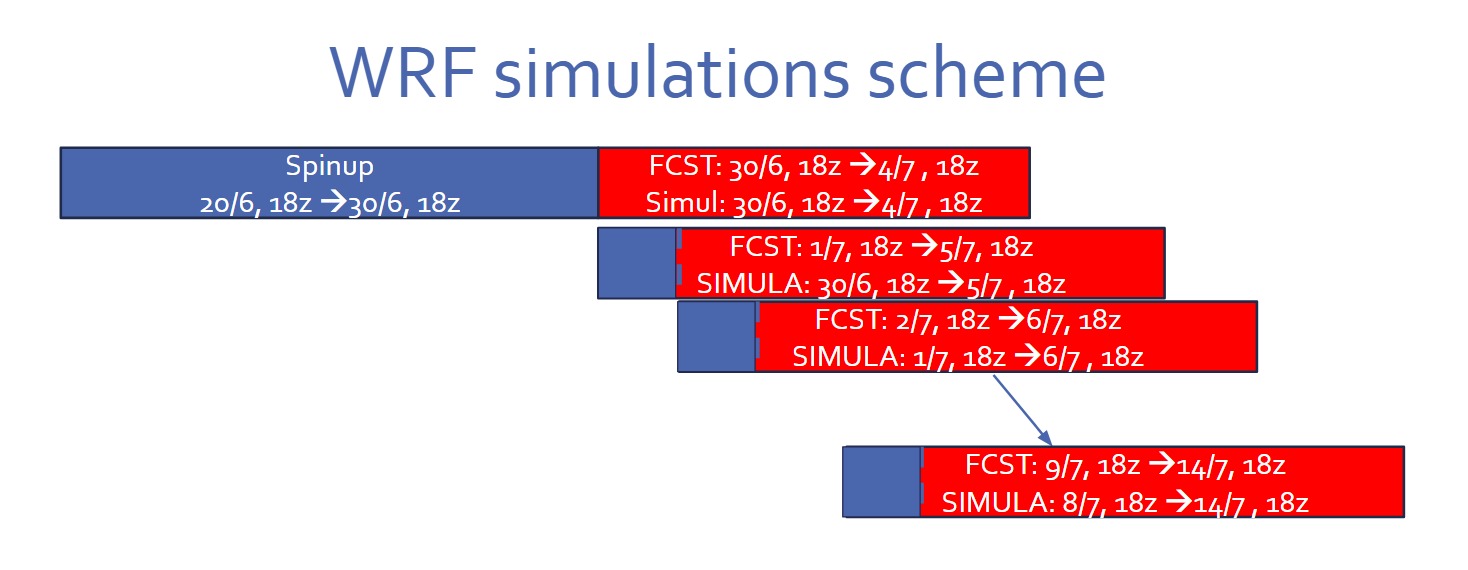
\includegraphics[width=\linewidth]{Figure_1.png}
	\caption{Forecasting scheme applied to the WRF and CHIMERE simulations. Red sections represent valid forecasting windows produced by each daily simulation.}
	\label{fig:Figure_1.png}
\end{wrapfigure}

For WRF, we tested six physical parameterizations, named by single-letter alphabetic acronyms,listed including a brief description of their employed schemes. A fully detailed list of the physics section employed for the namelist.input file can be found in Table 1:
\begin{itemize}
    \item A: Operational DMC (Chilean Meteorological Directorate) configuration
    \item B: Lapere *citation*
    \item C: Seguel/Bozkurt *citation*
    \item D: Proposed topographic correction
    \item E: Operational SERVIMET (Chilean Navy's Meteorological Service)
    \item F: Somosval *citation*
\end{itemize}

\begin{longtable}{@{}lcccccc@{}}
	
	\toprule
	Parameter & A & B & C & D & E & F \\
	\midrule
	\endfirsthead
	
	\toprule
	Parameter & A & B & C & D & E & F \\
	\midrule
	\endhead
	
	\midrule
	\multicolumn{7}{r}{Continued on next page} \\
	\endfoot
	
	\bottomrule
	\caption{Physical parametrizations considered for coupling with CHIMERE.}
	\label{tab:chimere_physics}
	\endlastfoot
	
	mp\_physics & 3 & 3 & 8 & 8 & 3 & 8 \\
	ra\_lw\_physics & 1 & 3 & 1 & 3 & 1 & 1 \\
	ra\_sw\_physics & 1 & 1 & 1 & 3 & 1 & 1 \\
	radt & 15 & 5 & 15 & 5 & 30 & 15 \\
	sf\_sfclay\_physics & 5 & 5 & 1 & 1 & 1 & 1 \\
	sf\_surface\_physics & 1 & 2 & 4 & 4 & 2 & 1 \\
	bl\_pbl\_physics & 5 & 5 & 5 & 1 & 1 & 1 \\
	bldt & 0 & 0 & 0 & 0 & 0 & 0 \\
	mp\_zero\_out & & & & & & 2 \\
	mp\_zero\_out\_thresh & & & & & & 1.e-8 \\
	cu\_physics & 5 & 5 & 5 & 5 & 1 & 2 \\
	cudt & 5 & 5 & 0 & 5 & 5 & 0 \\
	cugd\_avedx & & & & & & 1 \\
	isfflx & 1 & & 1 & 1 & 1 & 1 \\
	ifsnow & 0 & & 0 & & 1 & 0 \\
	icloud & 1 & 1 & 1 & 1 & 1 & 1 \\
	surface\_input\_source & 1 & & 1 & 1 & 1 & 1 \\
	num\_soil\_layers & 5 & & 4 & 5 & 4 & 4 \\
	topo\_wind & & & & 1 & & \\
	slope\_rad & & & & & 1 & \\
	topo\_shading & & & & & 1 & \\
	maxiens & & & & & & 1 \\
	maxens & & & & & & 3 \\
	maxens2 & & & & & & 3 \\
	maxens3 & & & & & & 16 \\
	ensdim & & & & & & 144 \\
	cu\_rad\_feedback & & & & & & .true. \\
	
\end{longtable}

WRF outputs were evaluated using the observational network from the
Chilean Meteorological Directorate (DMC) weather stations,
AMDAR aircraft profiles from the Pudahuel airport, radiosonde
measurements, and SINCA air quality monitoring stations, as shown in Figure 1.

\begin{wrapfigure}{r}{0.40\textwidth}
    \centering
    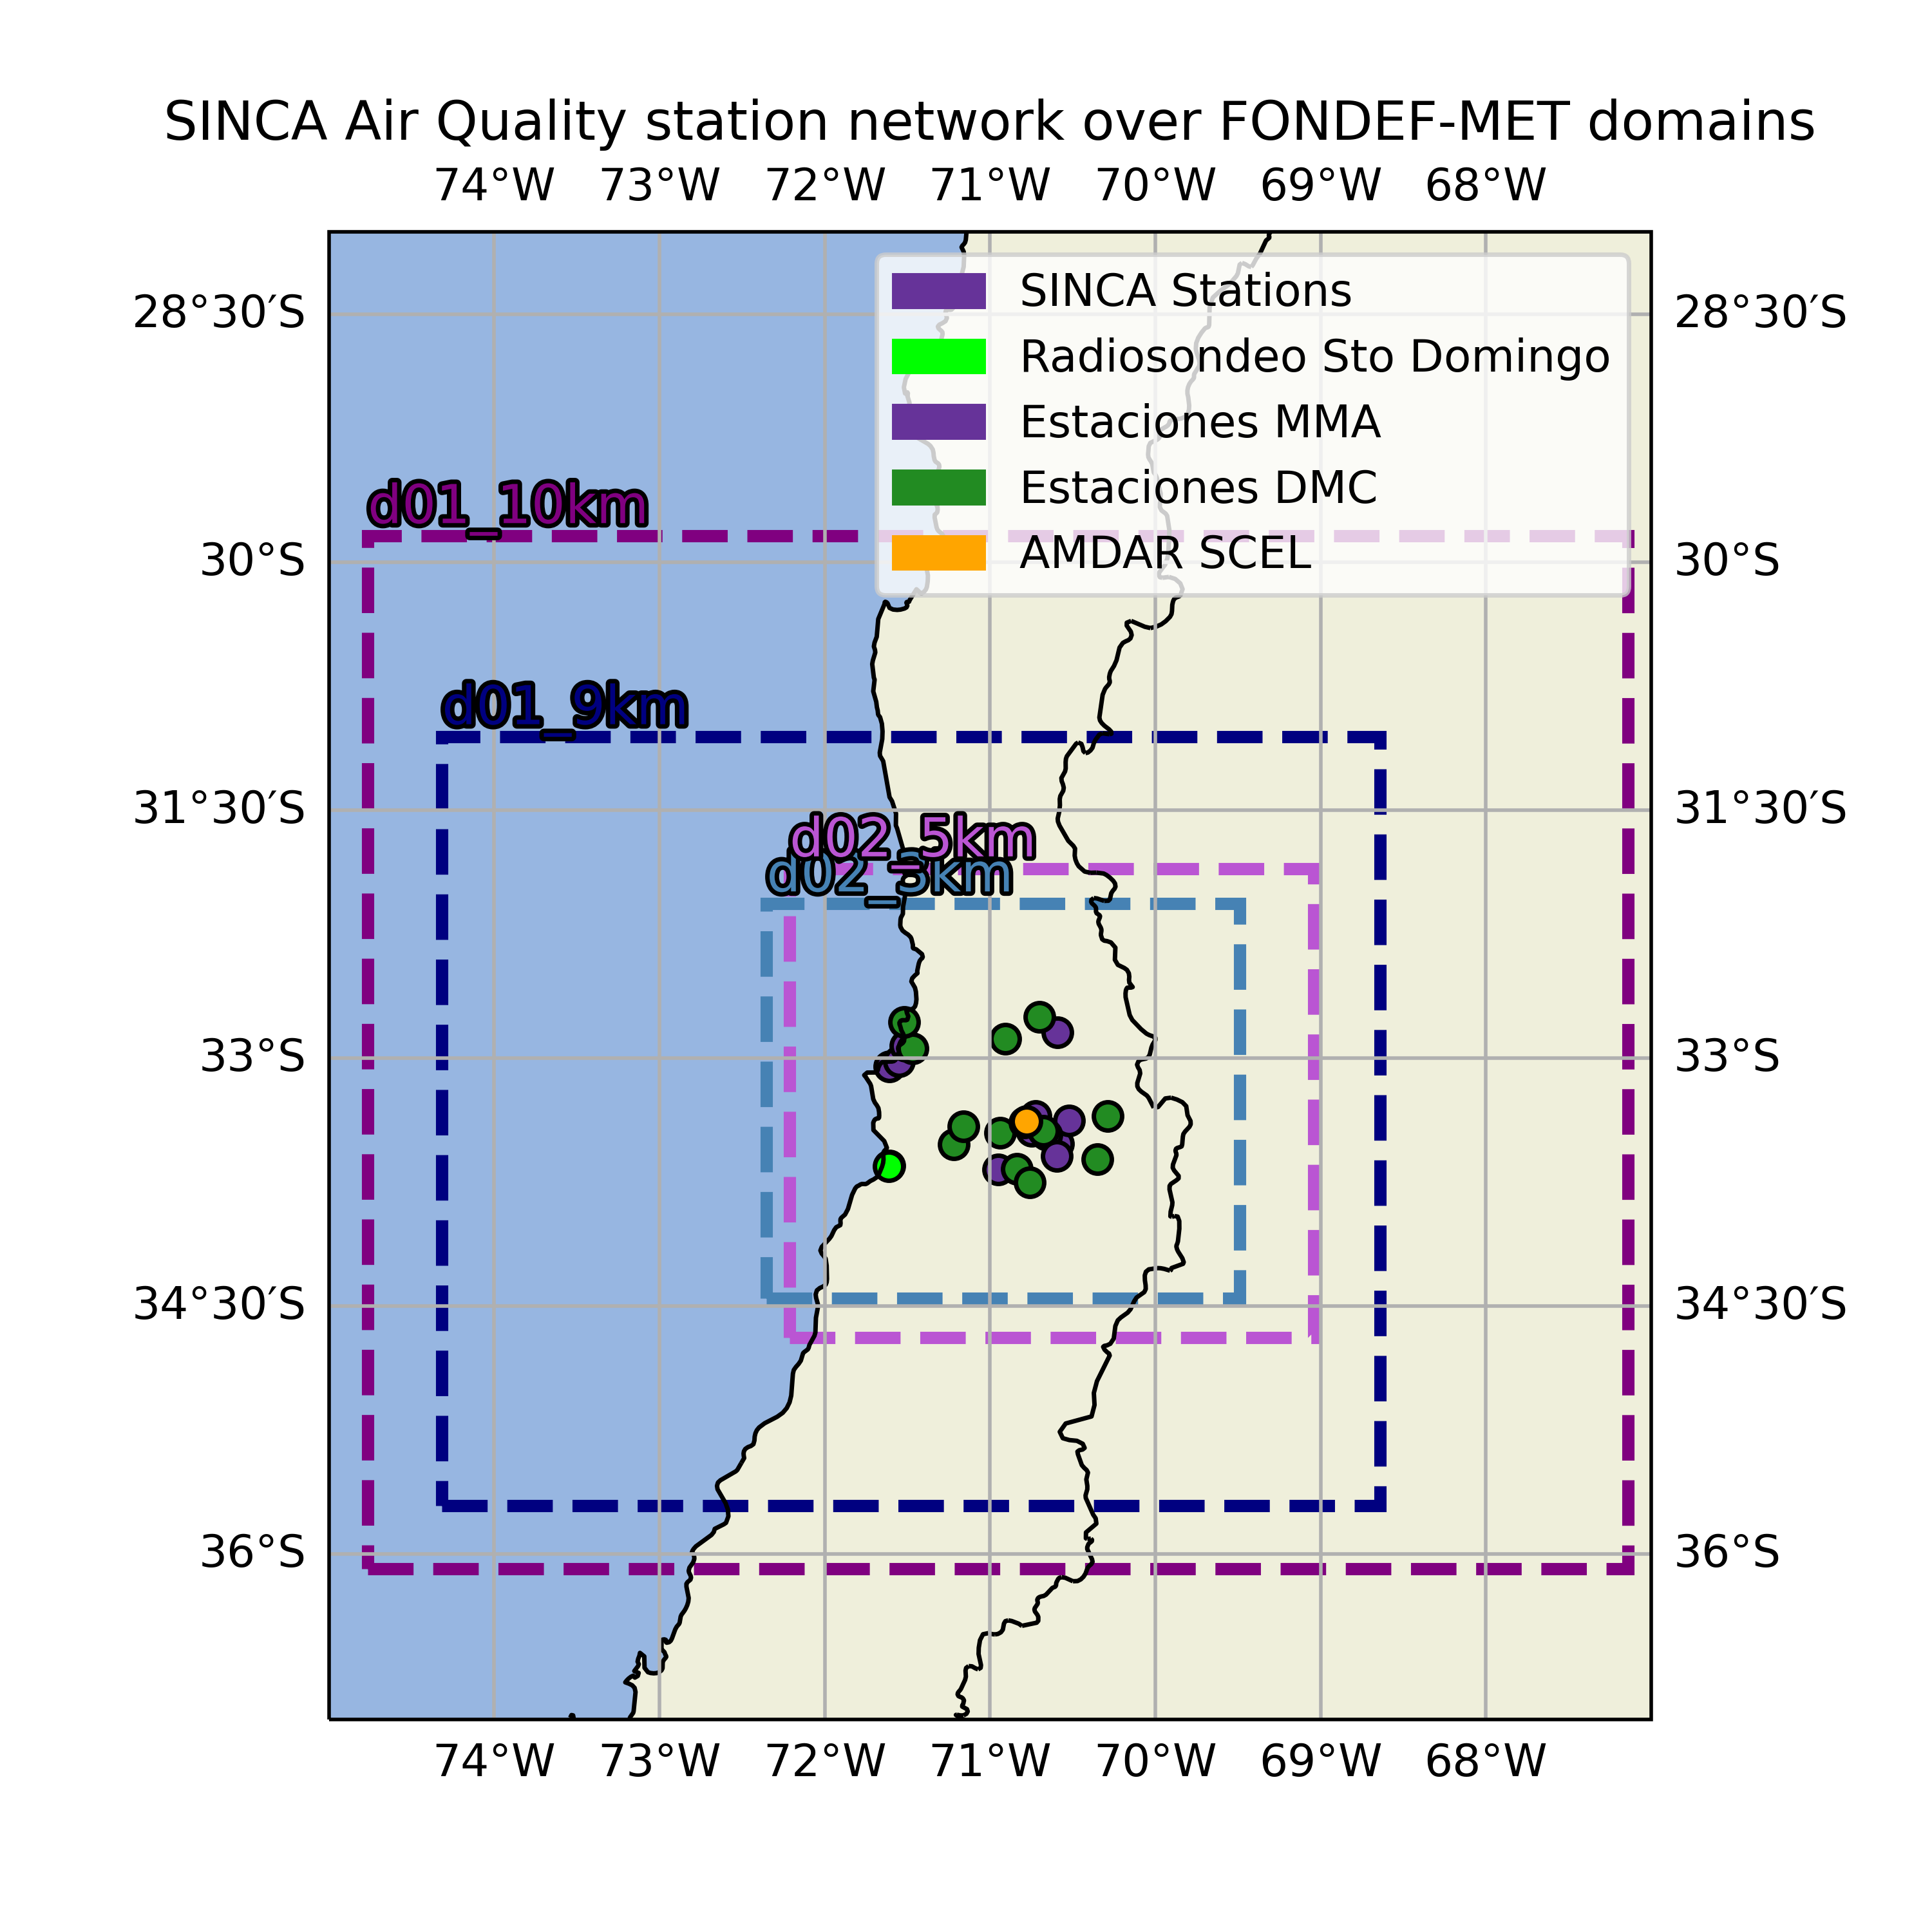
\includegraphics[width=\linewidth]{Figure_2.png}
    \caption{WRF domain configuration and observational network
used to evaluate meteorological simulations in Central Chile, including
DMC surface stations (dark green), AMDAR profiles (orange), radiosonde observations (located in Santo Domingo, OMM code 85586), and SINCA
monitoring sites (purple).}
    \label{fig:Figure_2.png}
\end{wrapfigure}


The forecast skill evaluation of the tested WRF configurations was based on traditional statistical metrics, consisting on:

\begin{itemize}
\tightlist
\item Normalized Root Mean Square Error (NRMSE)
\item Mean Bias Error (MBE)
\item Pearson correlation coefficient
\item Standard deviation ratio
\end{itemize}


These metrics were applied across different forecast lead times and
spatial resolutions.

Subsequently, and to simplify the decision on which
configuration is better suited to connect with the air quality
forecasting system, a \textbf{multiparametric ranking methodology} was
implemented to identify and efficiently communicate the results.

The ranking methodology was designed to provide an objective and
comprehensive evaluation of the different configurations of the WRF model by integrating their performance into monitoring stations, vertical
atmospheric layers, and forecast settings. The procedure consists of
four sequential stages, as illustrated in Figure 1.b.

First, time series are extracted from each WRF simulation for every
monitoring station and vertical model level. Surface variables are
evaluated using station-specific time series, while upper-air variables
are analyzed independently at each WRF vertical level. This organization
preserves the spatial and vertical variability of the model performance
and allows the evaluation to distinguish between near-surface and
free-tropospheric behavior. The extracted series are further grouped
according to the model configuration, horizontal resolution, and
forecast lead time.

In the second stage, statistical performance metrics are computed for
every station and vertical level. Four complementary metrics are
considered: the Normalized Root Mean Square Error (NRMSE), which
quantifies the magnitude of the prediction error; the Pearson
correlation coefficient (R), which measures the temporal agreement
between simulations and observations; the Mean Bias Error (MBE), which
evaluates systematic overestimation or underestimation; and the Standard
Deviation Ratio (SD Ratio), defined as the ratio between the simulated
and observed standard deviations, which assesses the model's ability to
reproduce the observed variability. Together, these metrics provide a
balanced description of both accuracy and variability.

The third stage consists of ranking the WRF configurations according to
their performance for each metric. A weighted scoring system is then
applied to combine the individual rankings into a single performance
score. The Normalized Root Mean Square Error (NRMSE) receives a weight
of 40\%, reflecting its importance as the primary measure of overall
forecast accuracy. The Pearson correlation coefficient contributes 30\%,
emphasizing the capability of the model to reproduce temporal
variability. The Mean Bias Error accounts for 20\%, penalizing
systematic deviations from observations, while the Standard Deviation
Ratio contributes the remaining 10\%, rewarding configurations that
accurately reproduce the observed variance.

Finally, the integrated scores are aggregated across the spatial and
vertical domains using a second weighting scheme that reflects the
relative importance of different atmospheric layers. Surface performance
contributes 40\% of the final score, the lower troposphere contributes
45\%, and the upper troposphere contributes 15\%. This weighting
prioritizes the atmospheric layers that are most relevant for air
quality applications while still accounting for the model's performance
throughout the atmospheric column.

This hierarchical methodology yields a single objective ranking for each
WRF configuration by combining multiple statistical indicators with
spatial and vertical performance. The approach minimizes the influence
of any individual metric while ensuring that the final ranking reflects
both forecast accuracy and the model's ability to reproduce the temporal
and vertical structure of the atmosphere.

\subsection{\texorpdfstring{\textbf{Chemical Modeling
System}}{Chemical Modeling System}}\label{chemical-modeling-system}

The CHIMERE model was coupled with WRF using the two highest-ranked
meteorological configurations identified through the ranking analysis.

The system was configured to forecast surface concentrations of PM25,
PM10, O3, CO, and NO2 over Central Chile. Simulations were performed
using different combinations of:

\begin{itemize}
\tightlist
\item
  Emission inventories (CAMS and INEMA)\\
\item
  Chemical boundary conditions
\end{itemize}

The objective was to evaluate system sensitivity and identify the main
sources of uncertainty associated with chemical forecasting.

\subsection{\texorpdfstring{\textbf{Temporal Forecast
Evaluation}}{Temporal Forecast Evaluation}}\label{temporal-forecast-evaluation}

Temporal performance was evaluated by comparing simulations against
observations from the SINCA monitoring network using hourly time series
from representative stations within the study domain.

The analysis focused on:

\begin{itemize}
\tightlist
\item
  Reproduction of the diurnal cycle\\
\item
  Representation of concentration peaks\\
\item
  Phase and magnitude errors\\
\item
  Episode persistence\\
\item
  Performance degradation with increasing forecast horizon
\end{itemize}

Additionally, critical pollution episodes were examined to assess the
operational capability of the system to anticipate poor air quality
events.

\subsection{\texorpdfstring{\textbf{Spatial
Evaluation}}{Spatial Evaluation}}\label{spatial-evaluation}

The ability of the system to reproduce the spatial variability of
atmospheric pollutants was evaluated through:

\begin{itemize}
\tightlist
\item
  Spatial comparisons between urban and rural monitoring stations\\
\item
  Evaluation of regional transport and ventilation patterns
\end{itemize}

\section{\texorpdfstring{\textbf{Results and discussion}}{Results and discussion}}\label{Results and discussion}
\textbf{WRF configuration ranking results}

\begin{figure}[htbp]
    \centering
    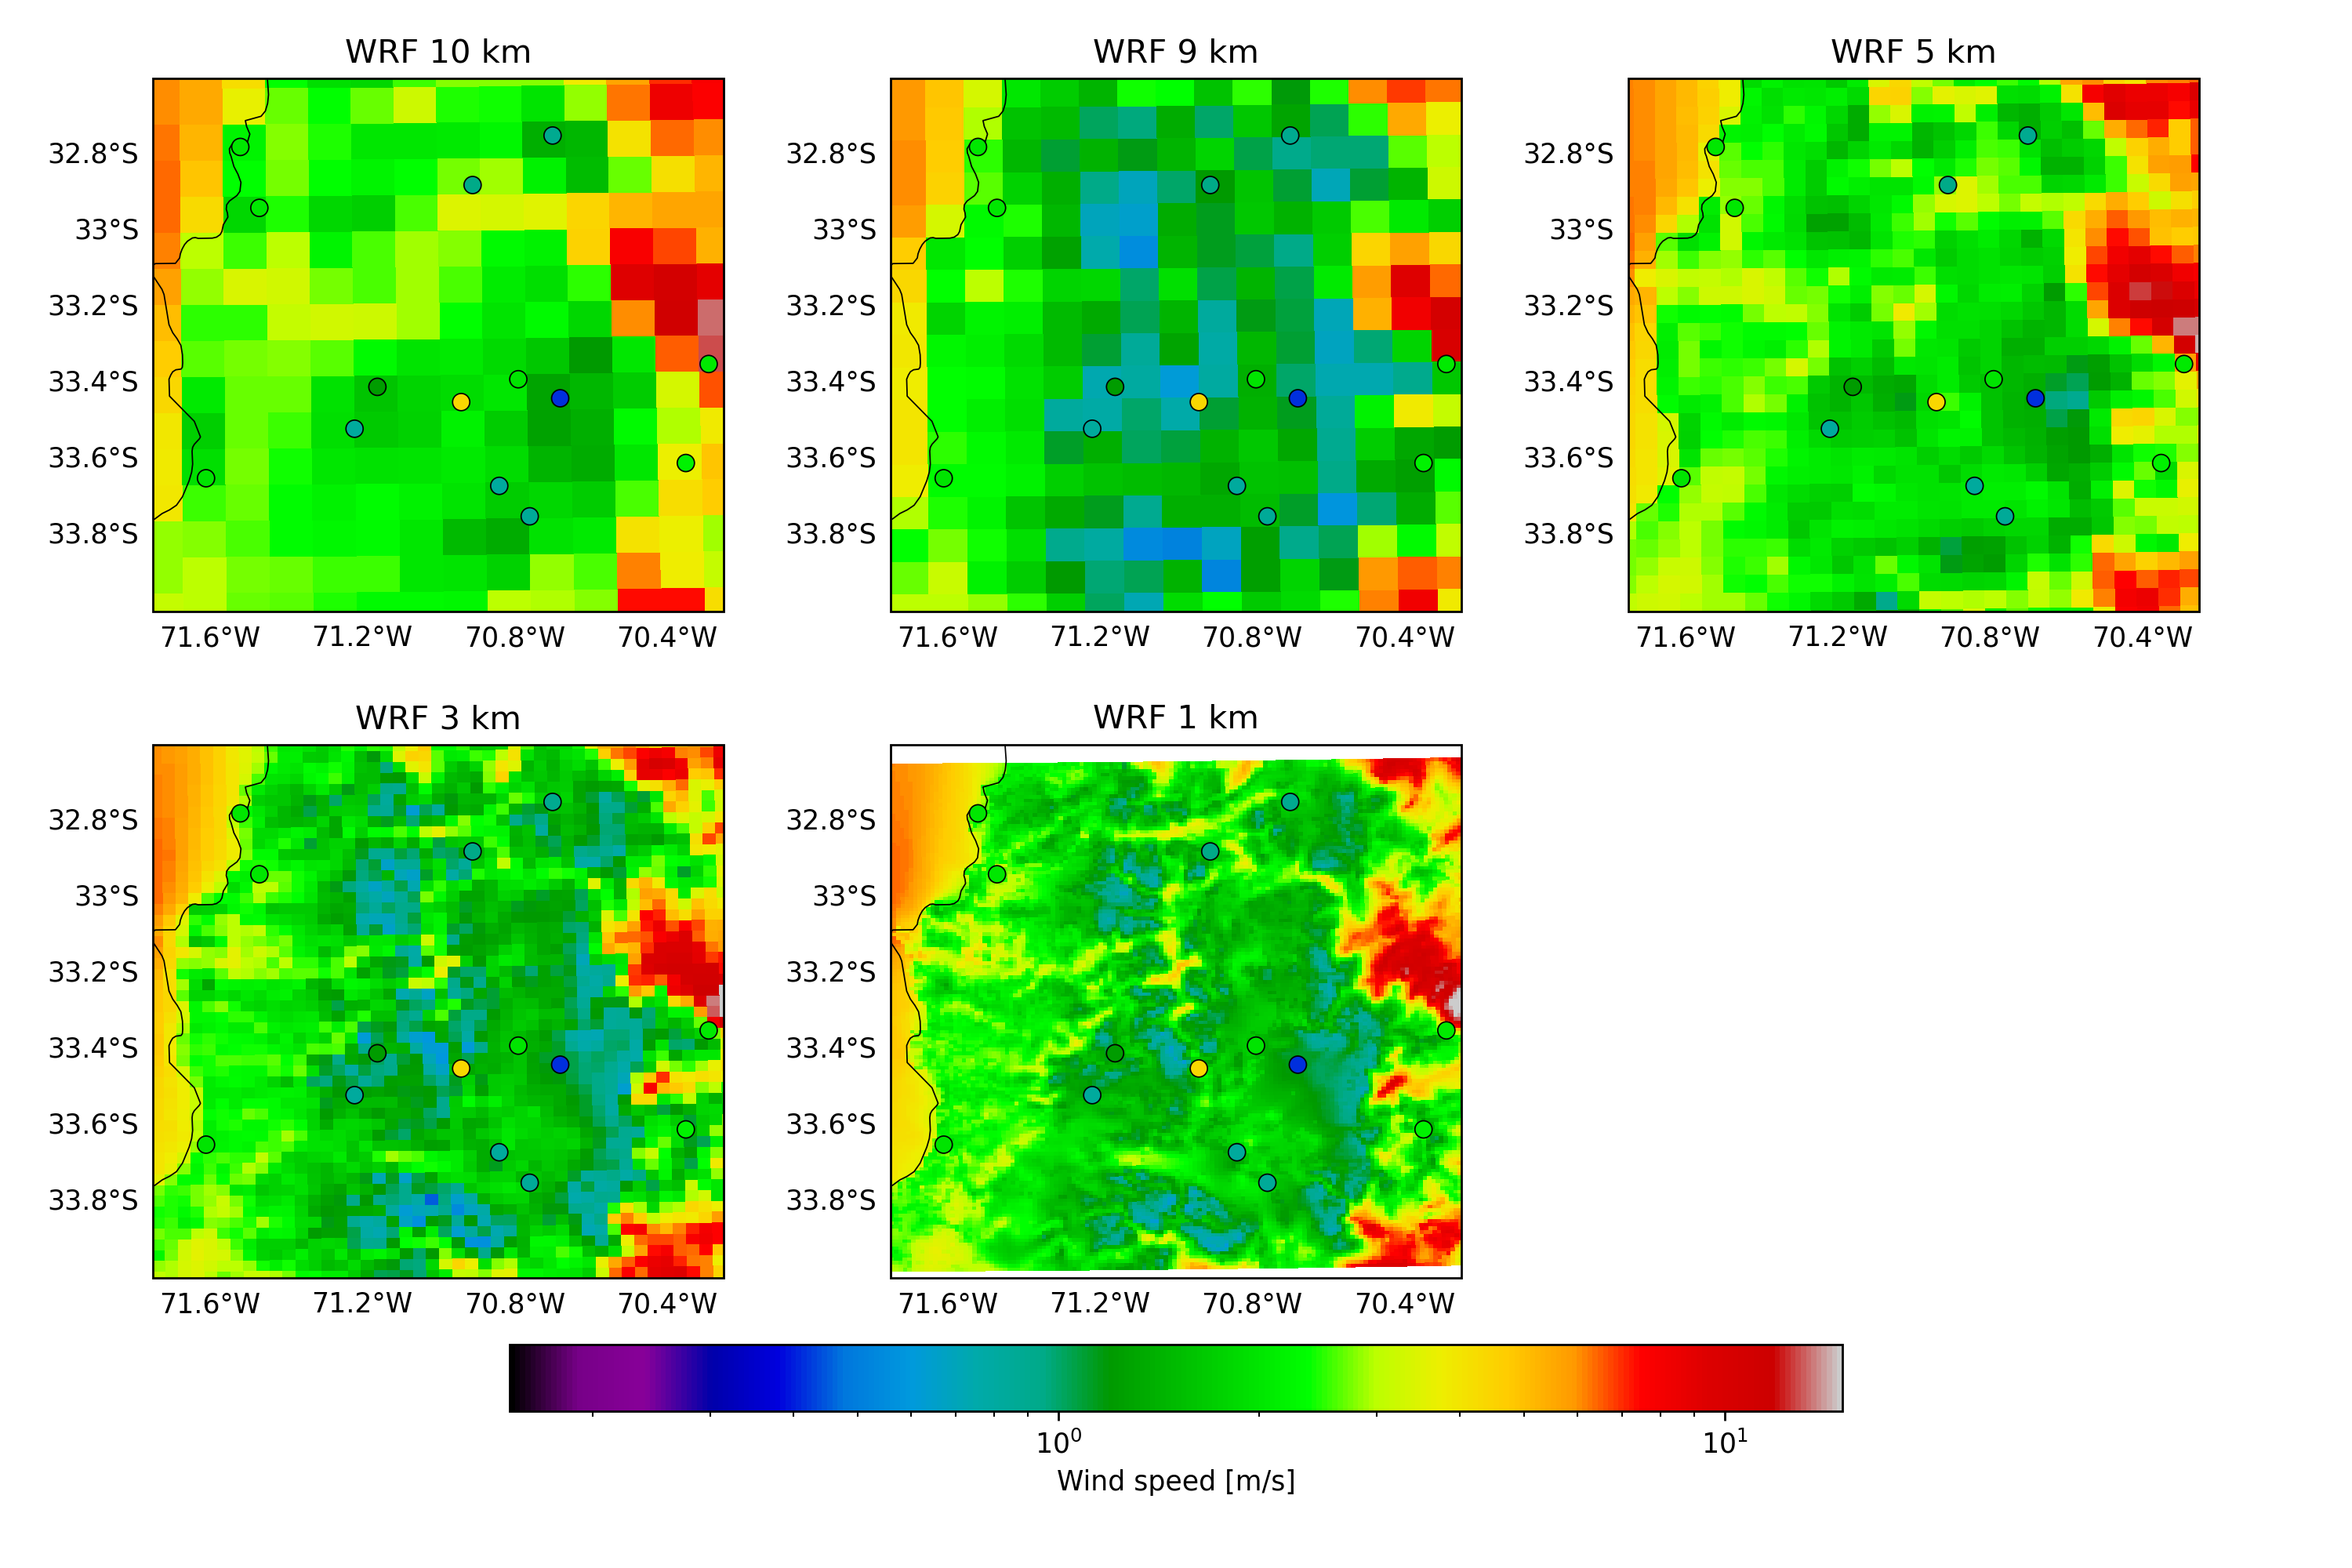
\includegraphics[width=\linewidth]{Figure_3.png}

    \textbf{Figure 3} Temporal mean of configuration C 10-meter wind speed fields across Central Chile (colormap), compared to the temporal mean of the station observations for the same period (scatterplots). Each subplot represents a resolution from the 10/5 and 9/3/1 respective simulations for a 24-hour leadtime. The associated temporal standard deviation is included in Annex 3.a, as well as fields for different lead times, the fields for wind direction, 2-meter temperature and relative humidity, and incoming solar radiation.
\end{figure}

In Figure 4, we present the results for wind speed and direction between the six WRF configuration, given their more direct involvement with pollutant dispersion. For each configuration, individual cell scores show the relative performance of the configuration compared to the others, for the same resolution and lead time.

\begin{figure}[htbp]
    \centering
    \begin{minipage}{0.48\textwidth}
        \centering
        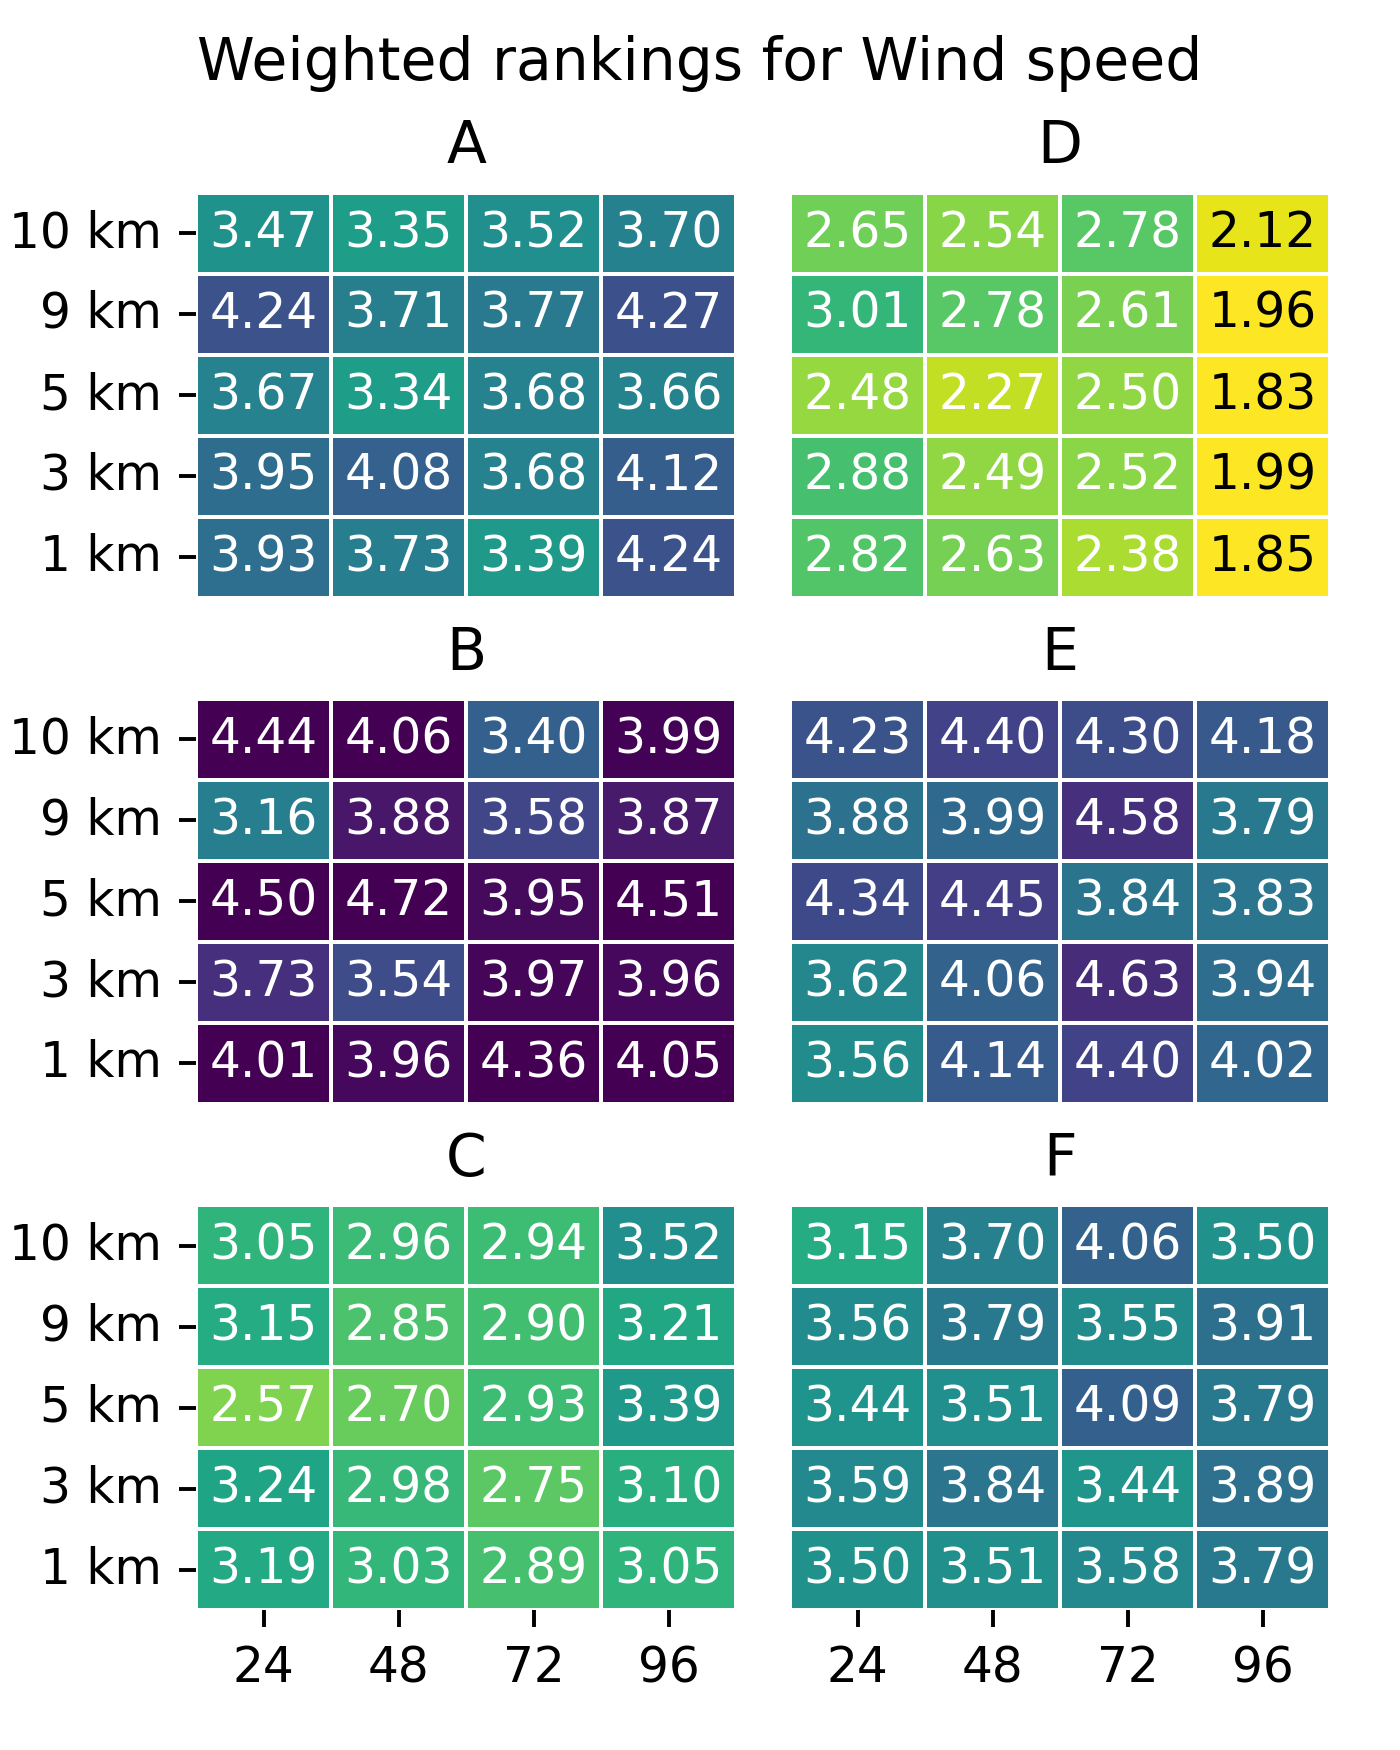
\includegraphics[width=\linewidth]{Figure_4.a.png}
   
    \end{minipage}
    \hfill
    \begin{minipage}{0.48\textwidth}
        \centering
        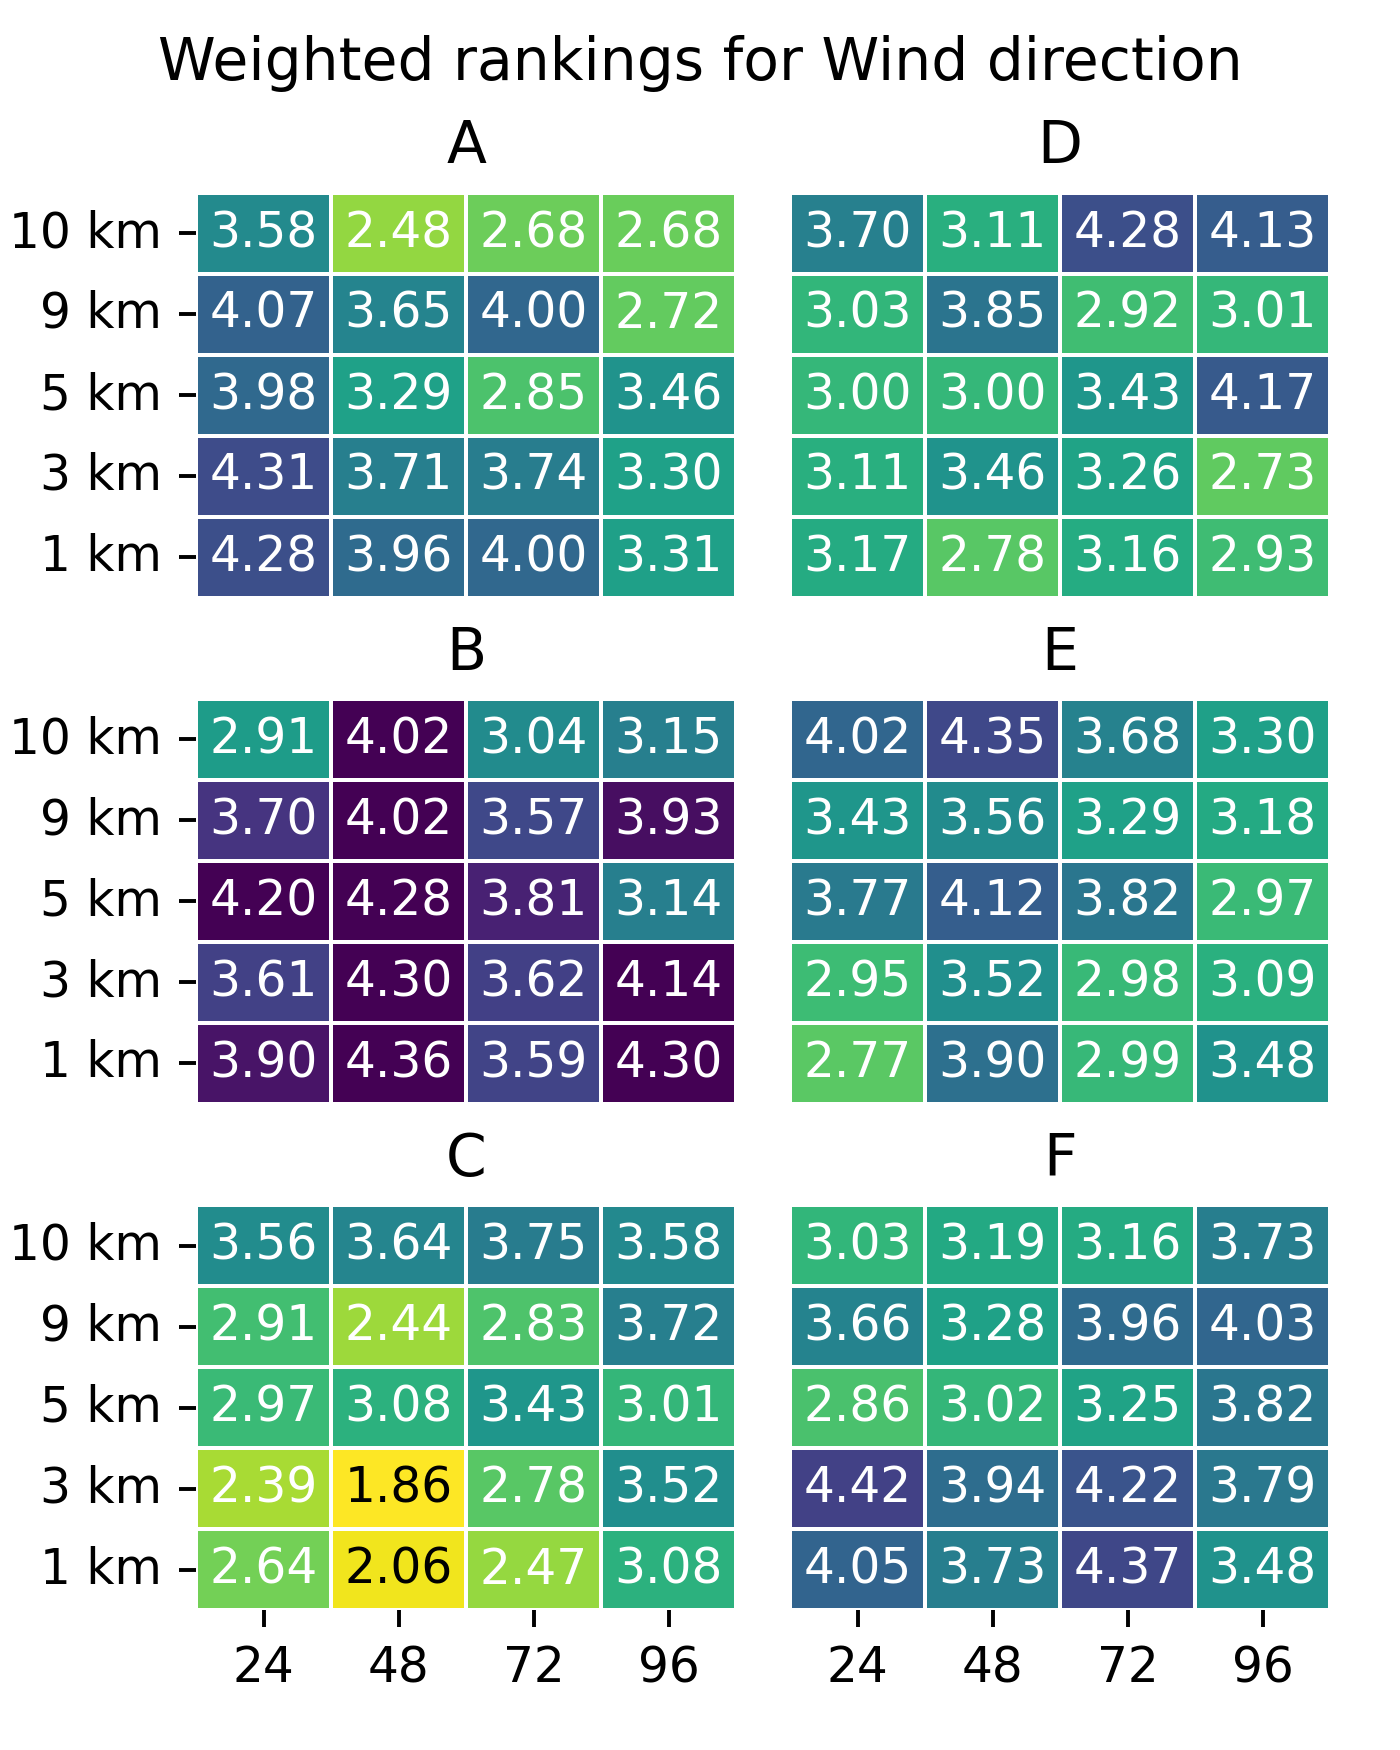
\includegraphics[width=\linewidth]{Figure_4.b.png}
  
    \end{minipage}
    \textbf{Figure 4} Statistical performance metrics used to evaluate WRF configurations for wind speed (left) and direction (right). Lower score indicates overall better performance relative to other ranked configurations for the same resolution and leadtime corresponding to each cell.
\end{figure}


Overall, D dominates in wind speed, arguably in relation to the topographic correction scheme. Nonetheless, this advantage is not as prominent for wind direction, in which C is actually the prevailing configuration at higher resolutions.

The WRF experiments showed that Central Chile's meteorology is strongly
controlled by the regional topography, coastal circulation, and seasonal
stability conditions. Across the tested configurations, the model
reproduced the broad spatial gradients of the observed meteorological
fields, with the best-performing setups (VENT, COAST) capturing both the
mean state and the main patterns of temporal variability. Differences
among configurations were generally modest at the synoptic scale but
became more evident in variables directly relevant for air-quality
forecasting, especially wind structure and boundary-layer evolution.

The multiparametric ranking procedure allowed us to distinguish
configurations that performed similarly under traditional summary
metrics but differed in their ability to represent vertical structure
and lead-time behavior. The selected top-ranked WRF configurations
provided the most balanced performance across surface and upper-air
variables, making them suitable for coupling with CHIMERE.


\begin{figure}[htbp]
	\centering
	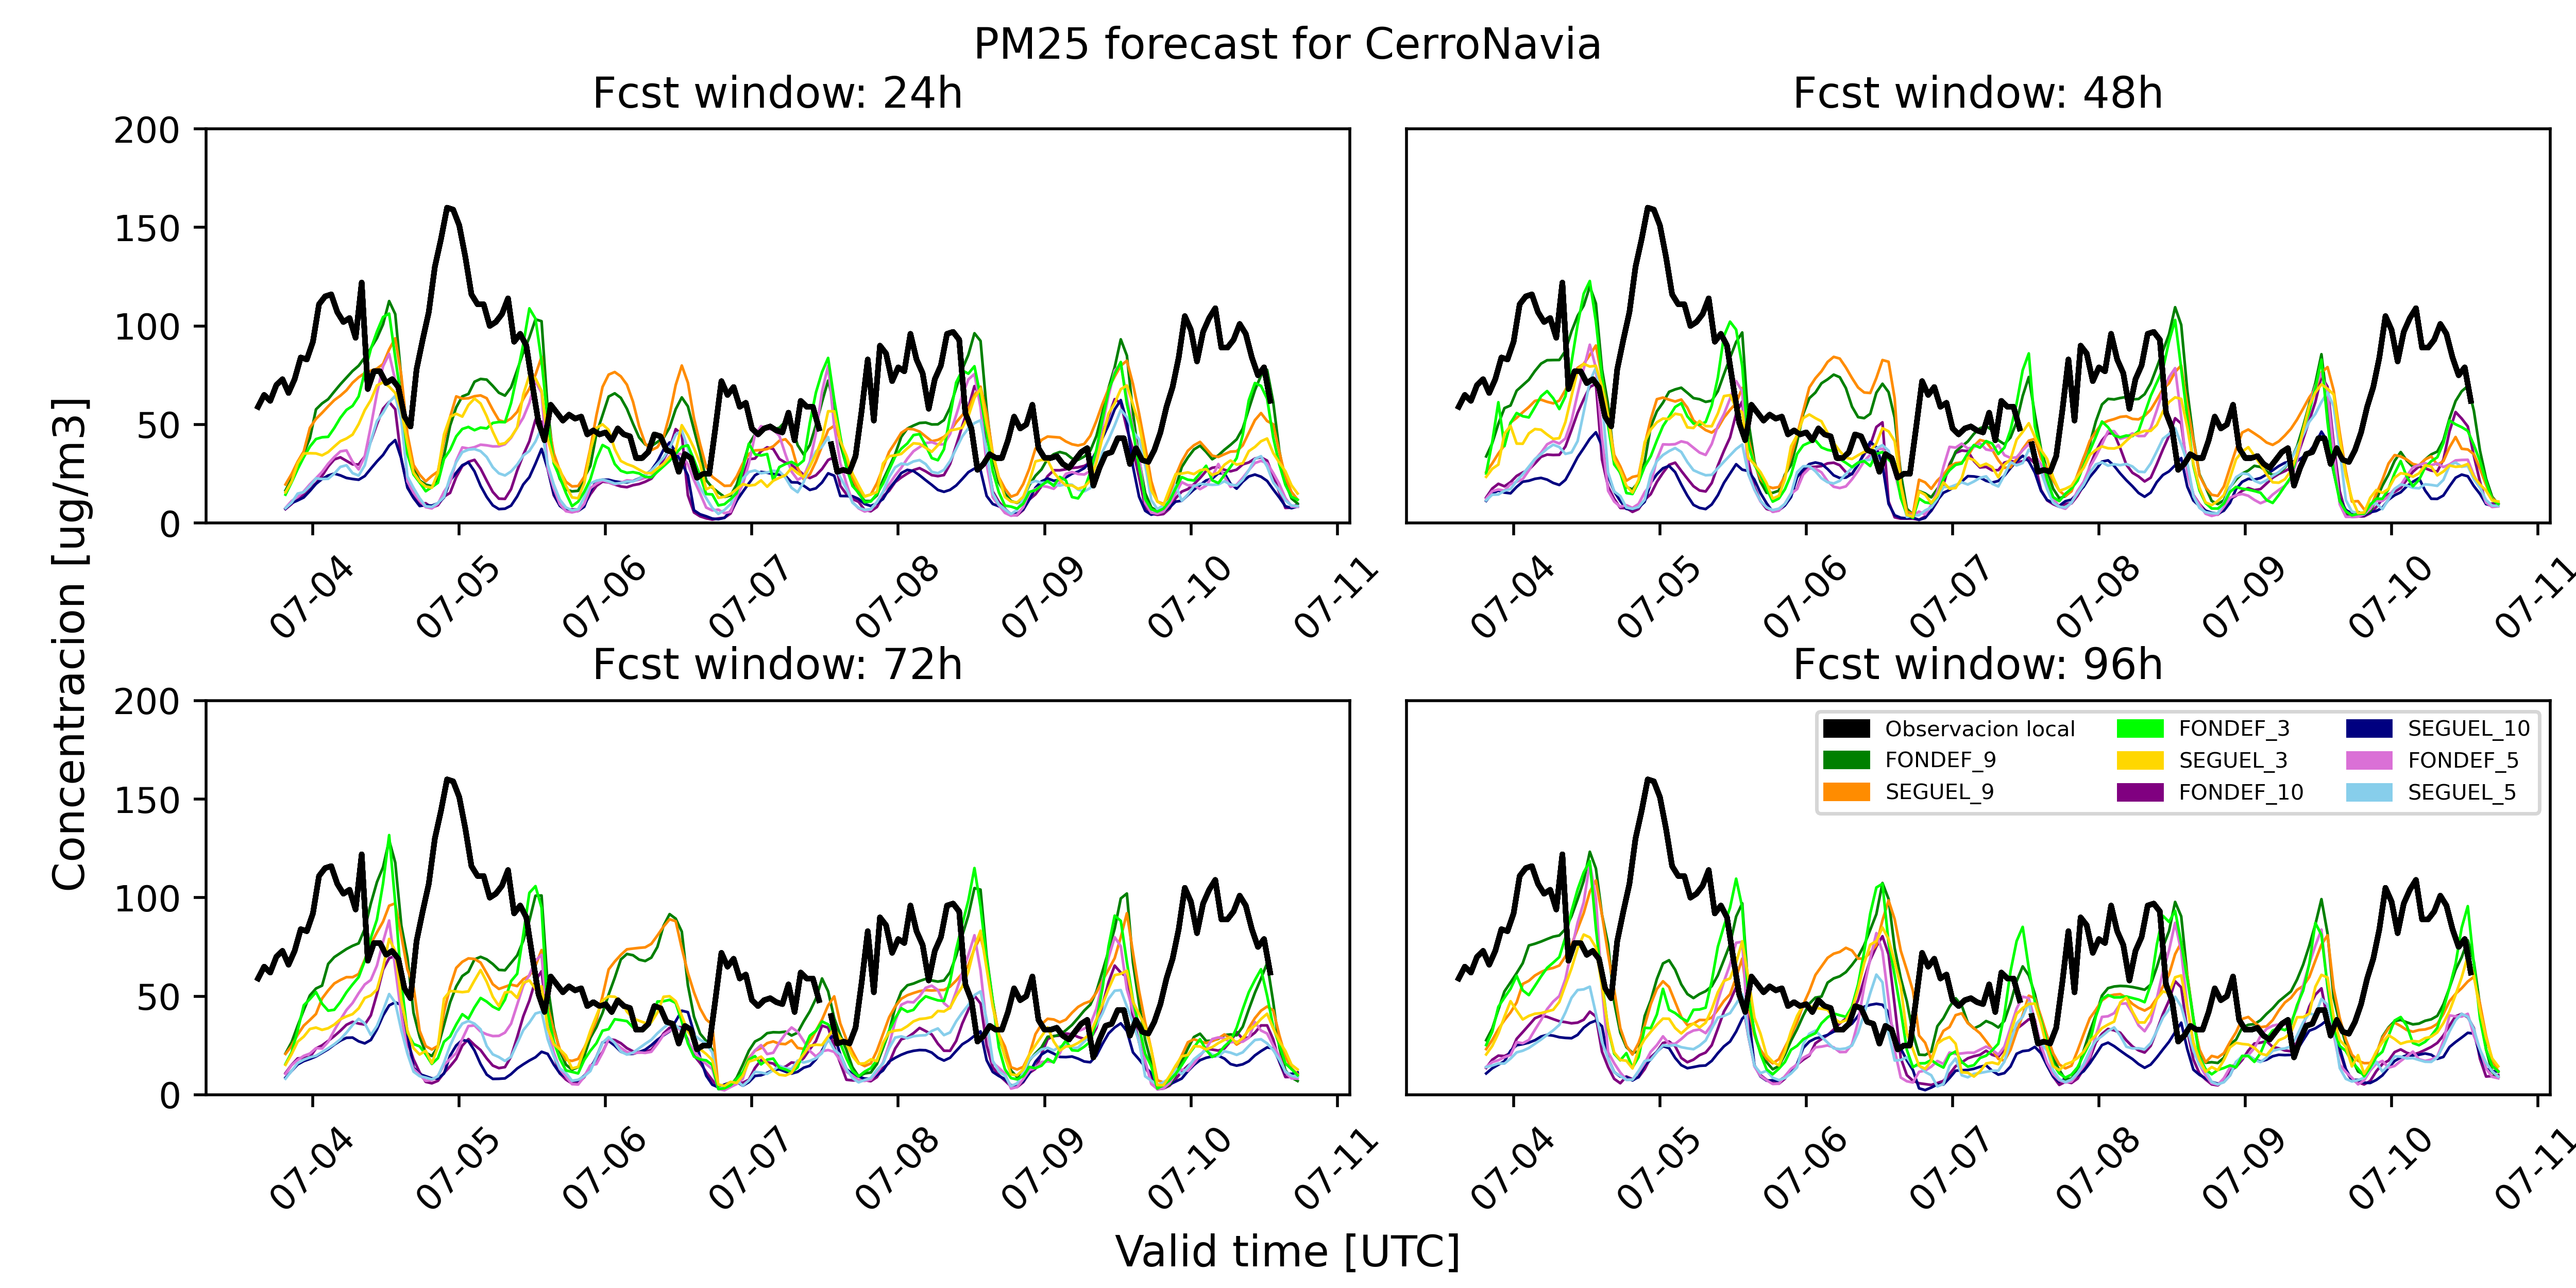
\includegraphics[width=0.99\textwidth]{Figure_5.a.png}
	\textbf{Figure 5.a} Forecast time series of PM25 concentrations from the coupled WRF-CHIMERE system at the Cerro Navia SINCA station. Each subplot represents a leadtime (labeled in the subplot's title), showing observed (black) and forecasted time series (colors by configuration/resolution). These forecasts are simulated from the INEMA emission inventory.
	\label{fig:figure5}
\end{figure}

\begin{figure}[htbp]
	\centering
	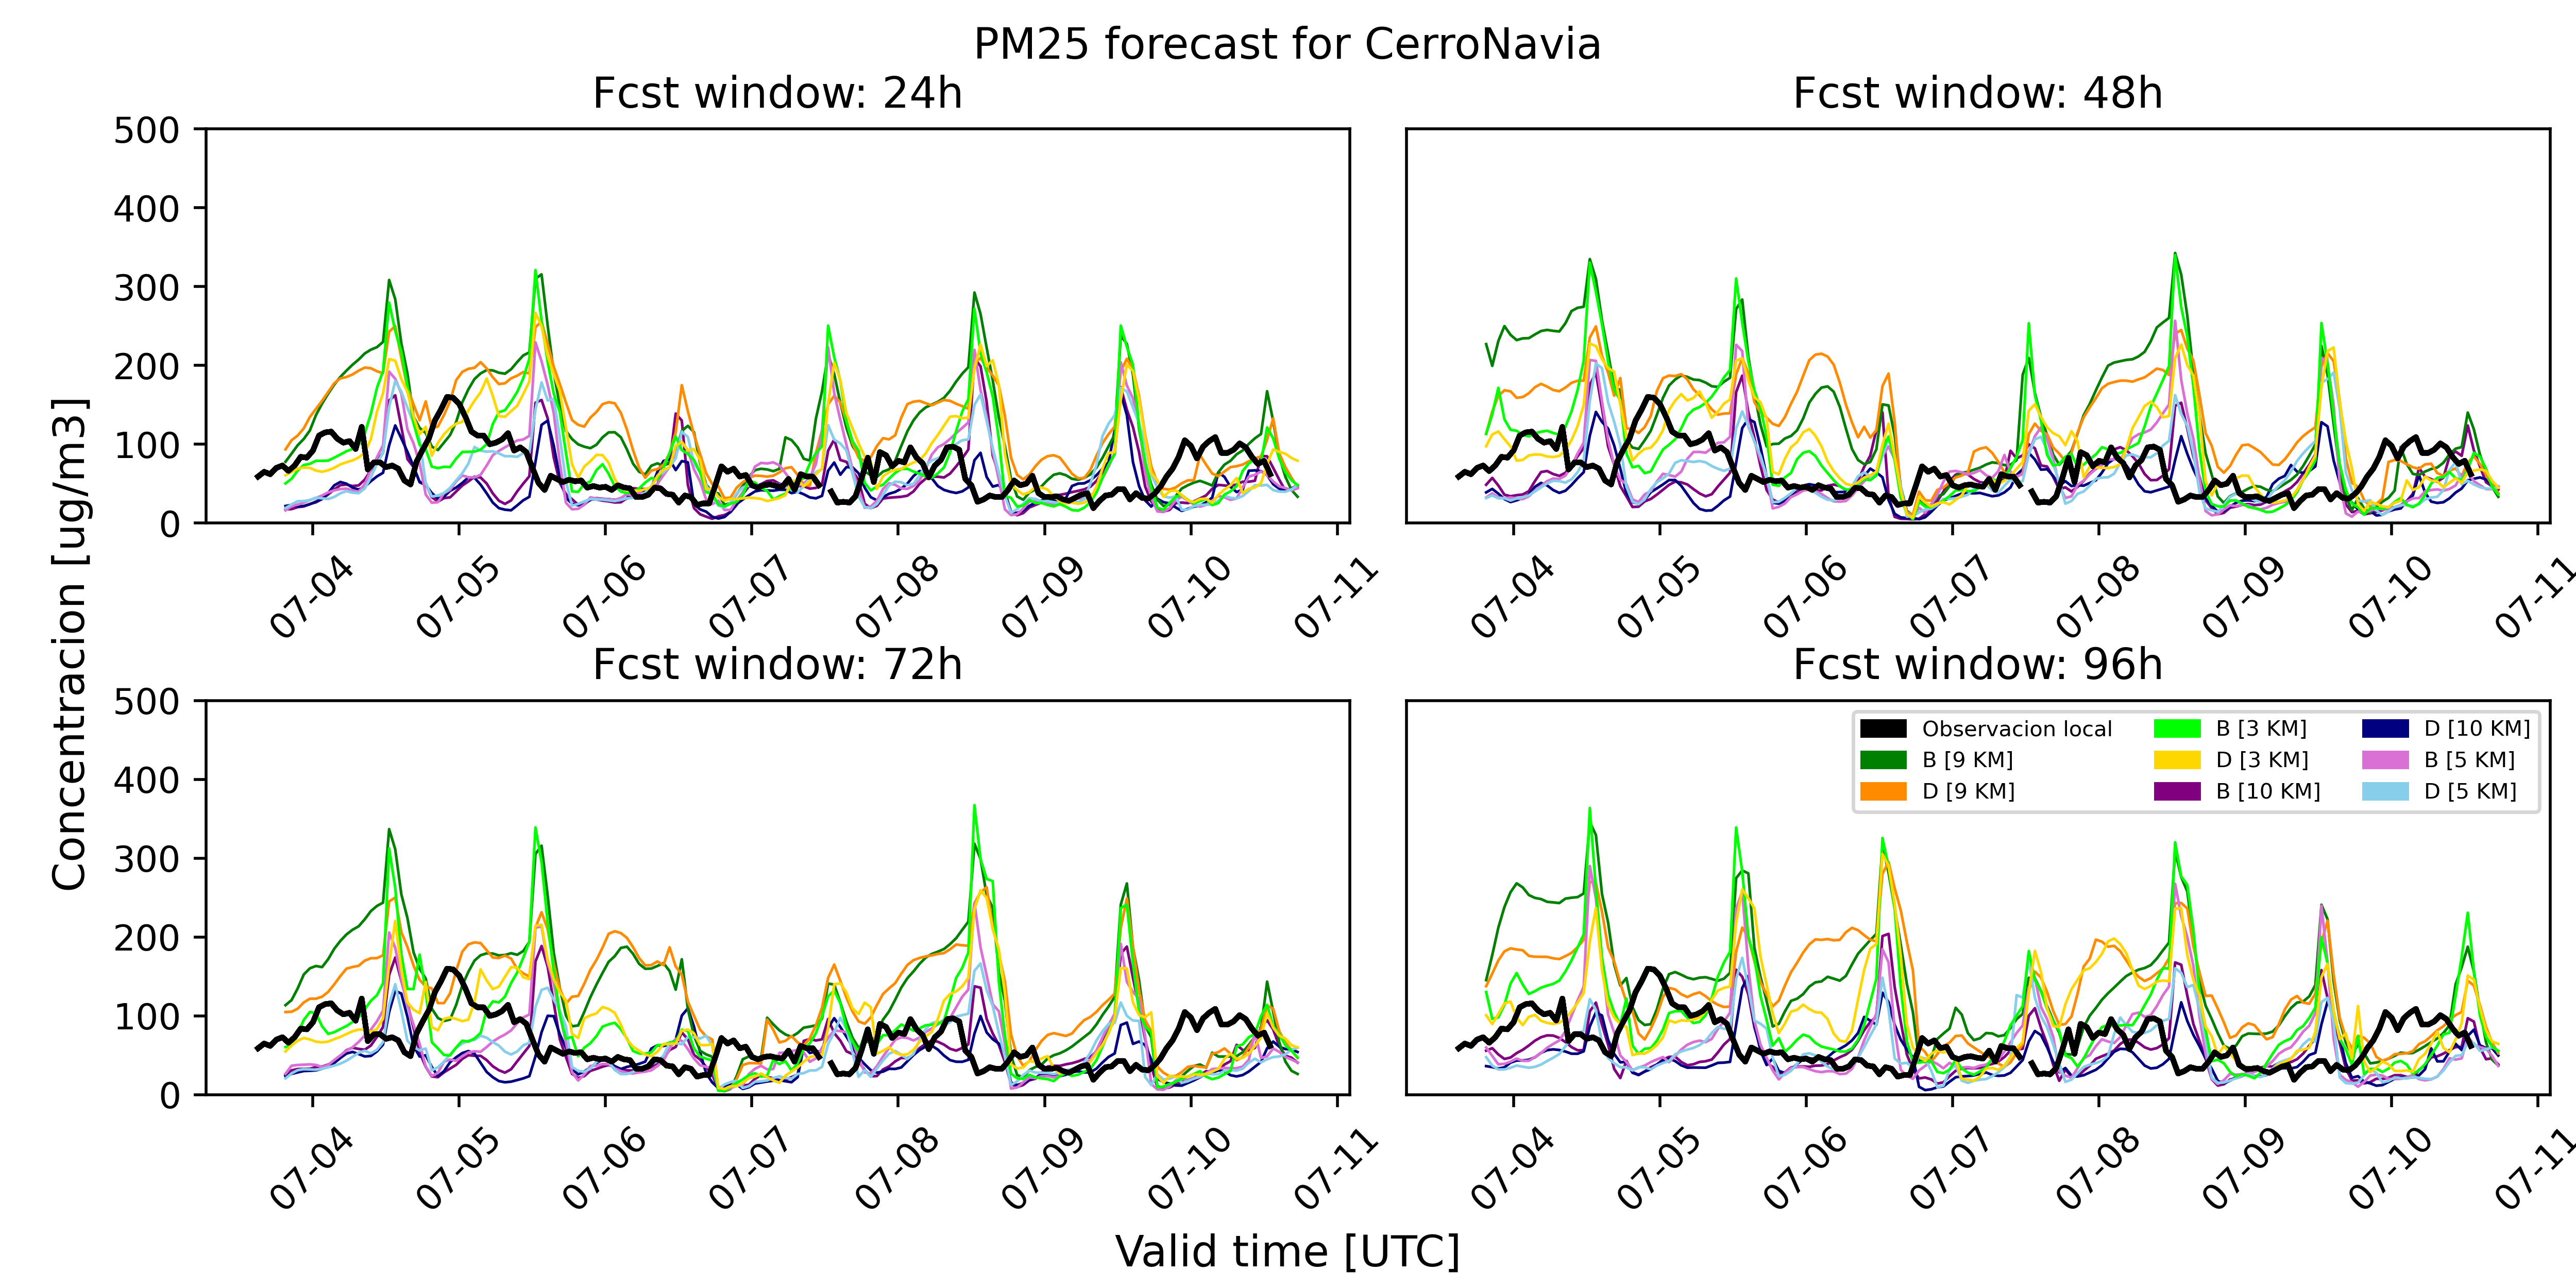
\includegraphics[width=0.99\textwidth]{Figure_5.b.png}
	\textbf{Figure 5.b} Forecast time series of PM25 concentrations from the coupled WRF-CHIMERE system at the Cerro Navia SINCA station. Each subplot represents a leadtime (labeled in the subplot's title), showing observed (black) and forecasted time series (colors by configuration/resolution). These forecasts are simulated from the CAMS emission inventory.
	\label{fig:figure5}
\end{figure}

\begin{figure}[htbp]
    \centering
    \begin{minipage}{0.49\textwidth}
        \centering
        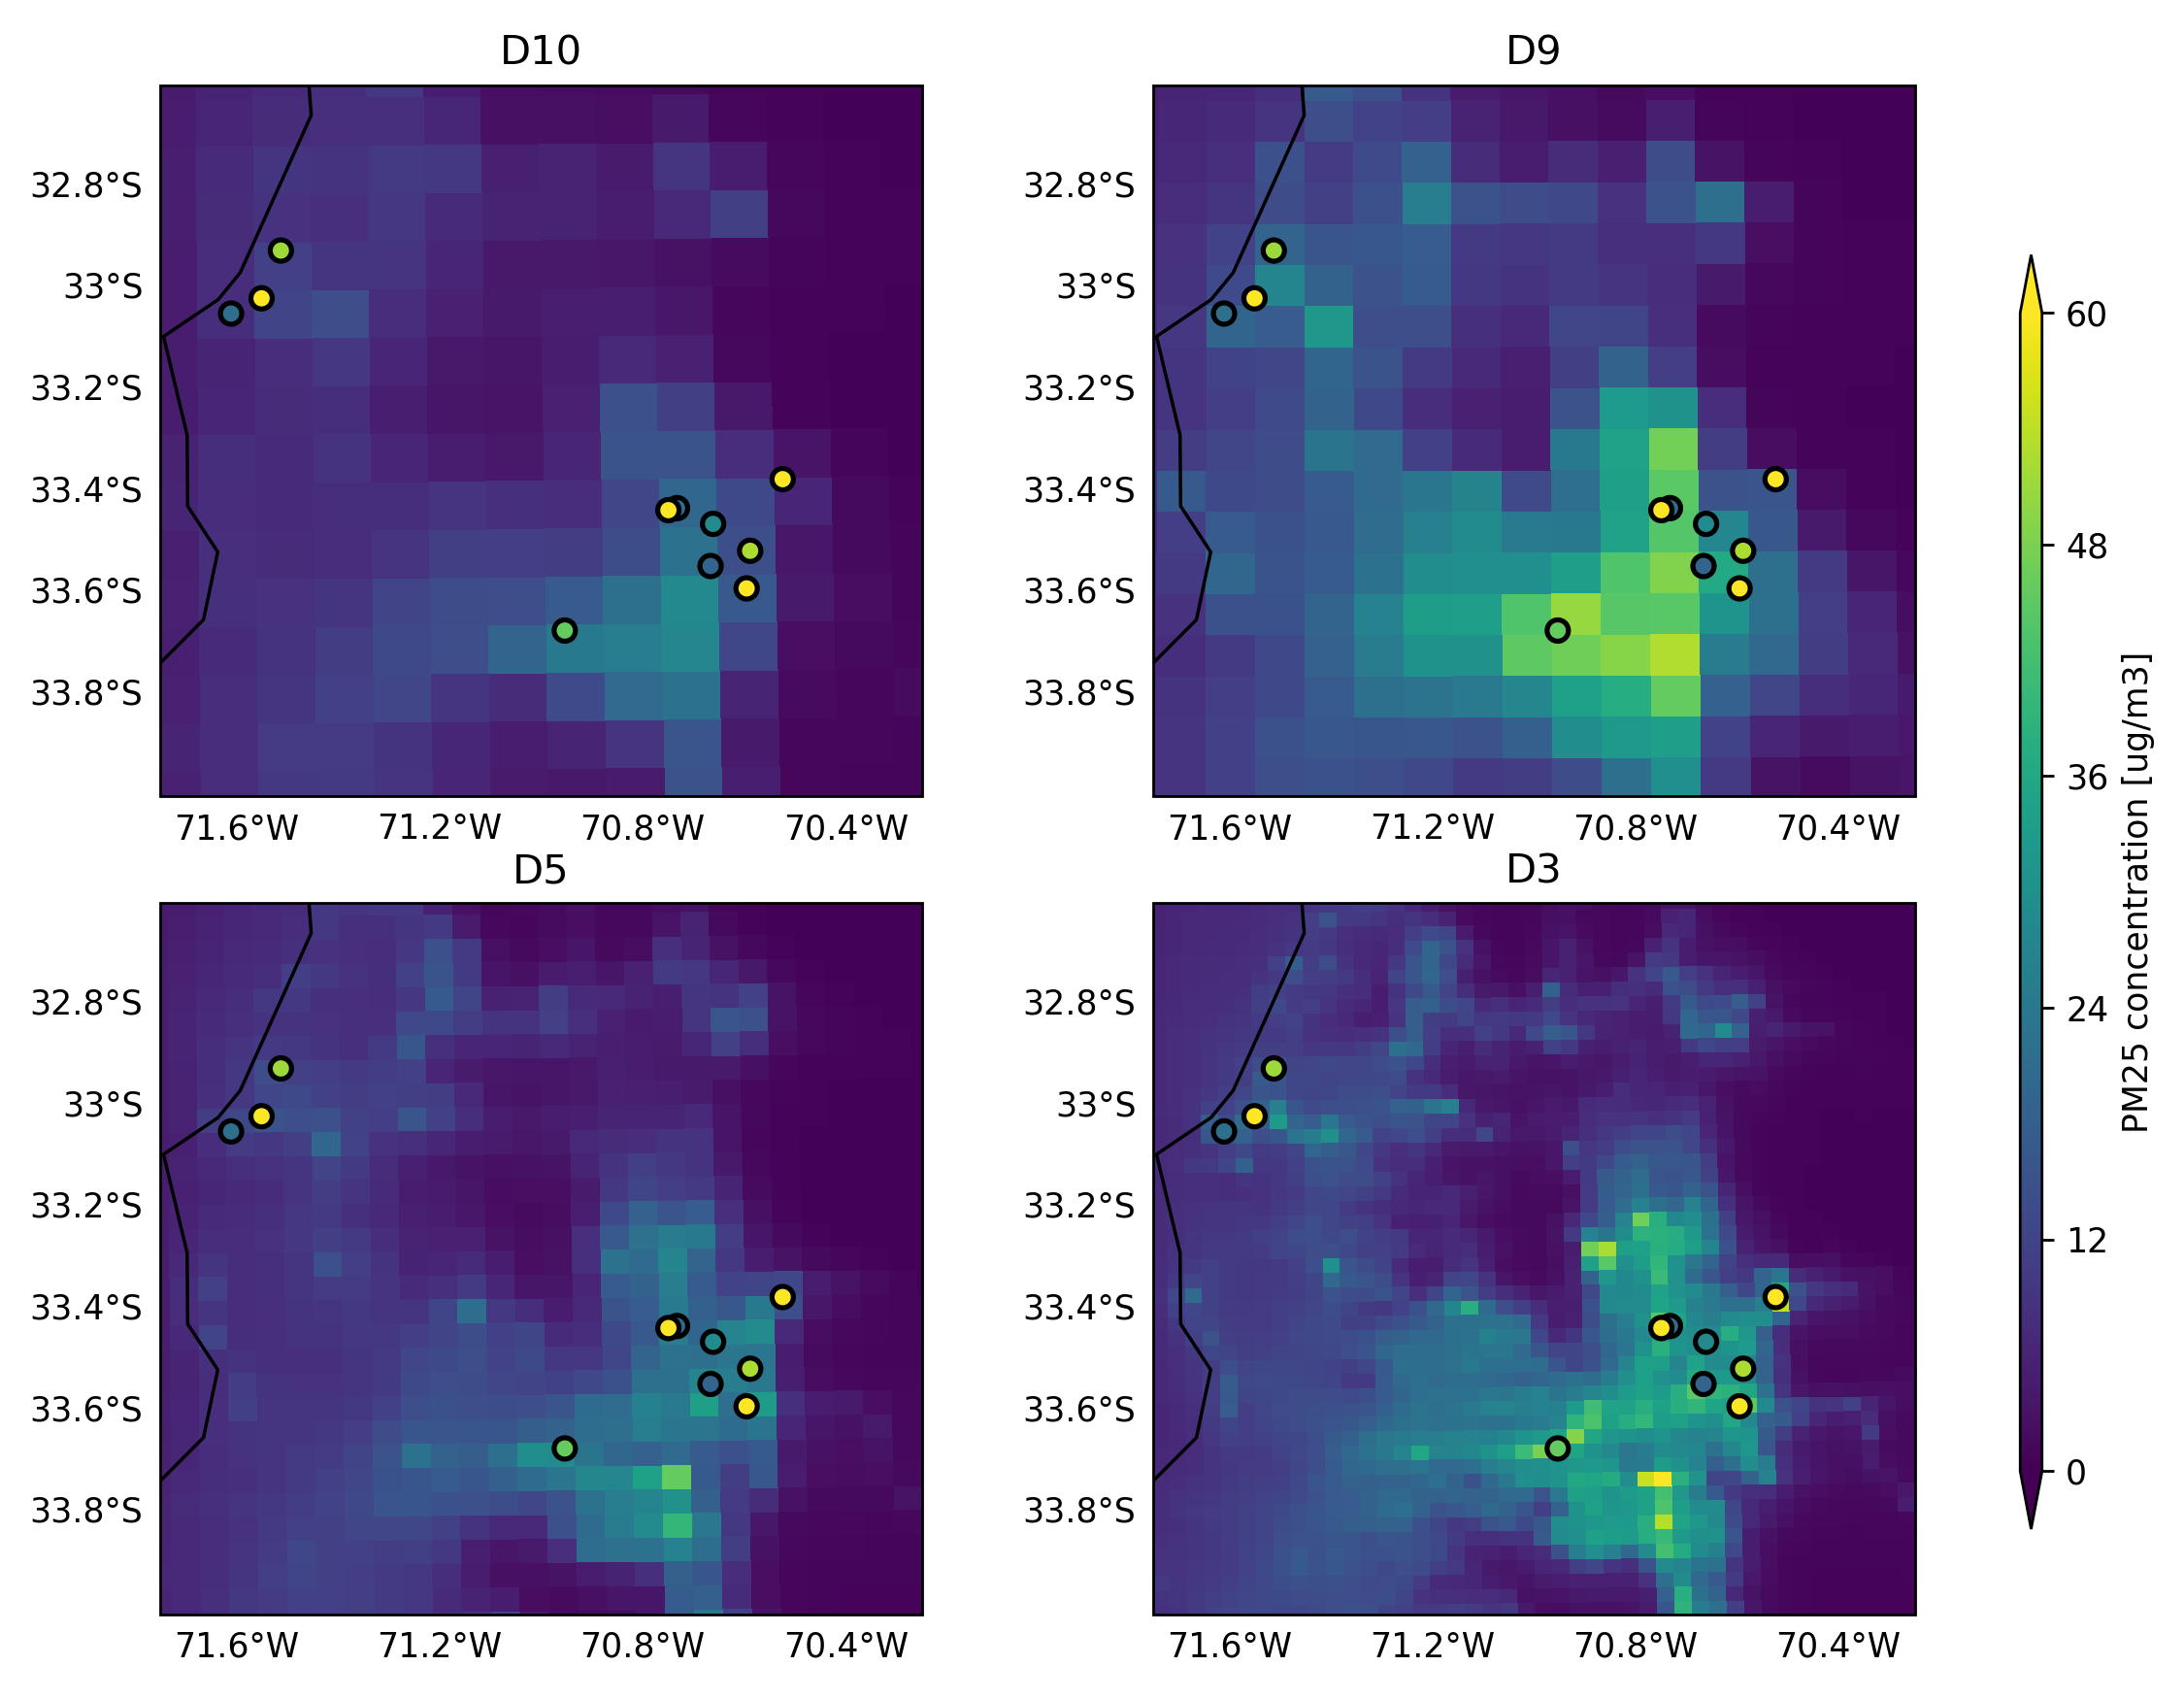
\includegraphics[width=\linewidth]{Figure_6.a.png}
    \end{minipage}
    \hfill
    \begin{minipage}{0.49\textwidth}
        \centering
        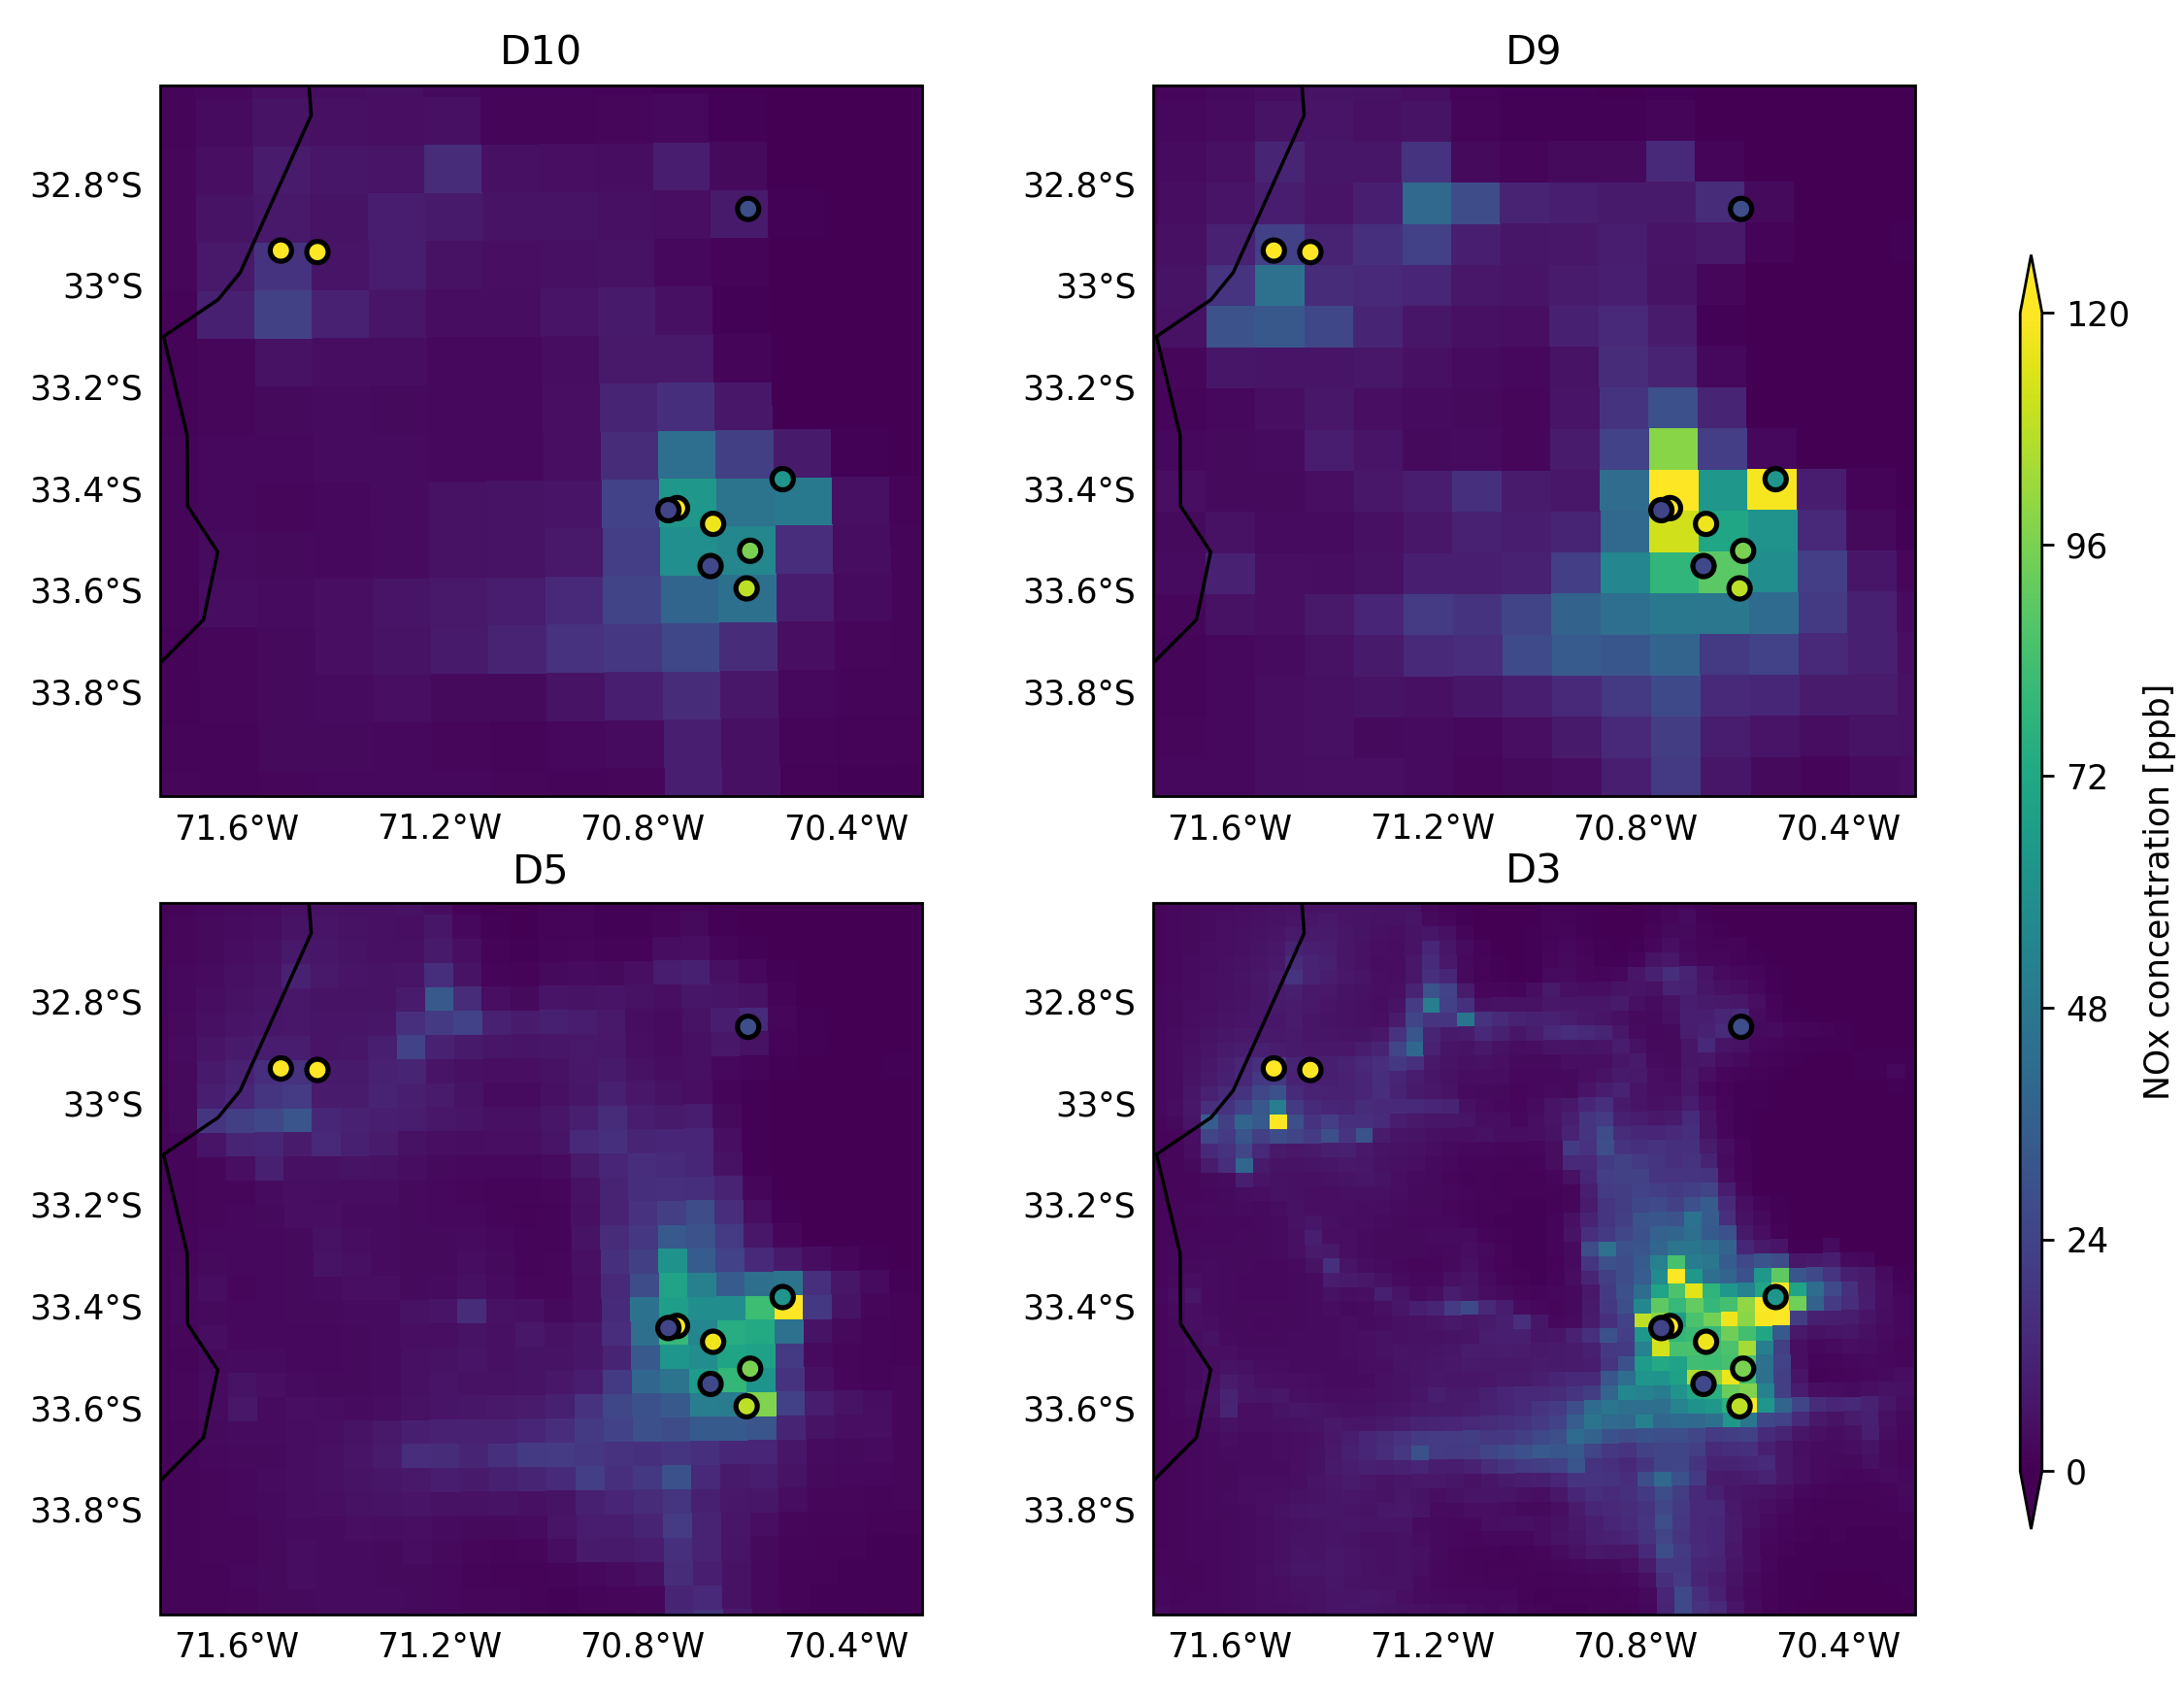
\includegraphics[width=\linewidth]{Figure_6.b.png}
    \end{minipage}
    \textbf{Figure 6} Temporal mean of PM25 (left) and NOx (right) concentrations from the coupled WRF--CHIMERE system, compared to SINCA stations (scatter plots). These fields were derived from the C WRF configuration and the INEMA emission inventory. Fields for the configuration D might be found in Annex 6.
\end{figure}

The coupled WRF--CHIMERE system successfully reproduced the main
temporal evolution of pollutant concentrations in Central Chile,
including the diurnal cycle and the occurrence of high-pollution
episodes. Skill was highest for pollutants and stations most directly
influenced by large-scale transport and basin-scale ventilation, while
larger discrepancies appeared under strongly stagnant conditions and
during episodes governed by local emissions and unresolved sub-grid
processes. Forecast quality decreased with lead time, but the system
retained useful skill over the operational forecast window.


Spatially, the model captured the contrast between accumulation zones in
the Santiago basin and better-ventilated surrounding areas. The
simulations also reproduced the regional influence of transport,
particularly under wintertime stability conditions when pollutants were
more likely to persist and accumulate. Sensitivity experiments using
different emissions inventories and boundary conditions showed that
model performance was meaningfully affected by these inputs, confirming
their importance as major sources of uncertainty in operational
forecasting.

To evaluate the spatial performance of the meteorological simulations,
the temporal mean and temporal standard deviation of the modeled
variables were compared with observations at all monitoring stations
(Figures XX--XX). While the mean fields characterize the climatological
state reproduced by the model, the standard deviation provides
information on its ability to represent temporal variability and
meteorological fluctuations.

The spatial distribution of the temporal mean indicates that the WRF
configurations successfully reproduce the large-scale spatial gradients
observed across Central Chile. For most variables, the observed station
values closely follow the simulated background field, indicating that
the model captures the first-order influence of topography, land--sea
contrasts, and regional circulation patterns on the climatological
state. Remaining discrepancies are generally localized and tend to occur
at stations situated in areas of complex terrain, where unresolved
topographic effects and local circulations become increasingly
important.

\begin{figure}[htbp]
    \centering
    \begin{minipage}{0.495\textwidth}
        \centering
        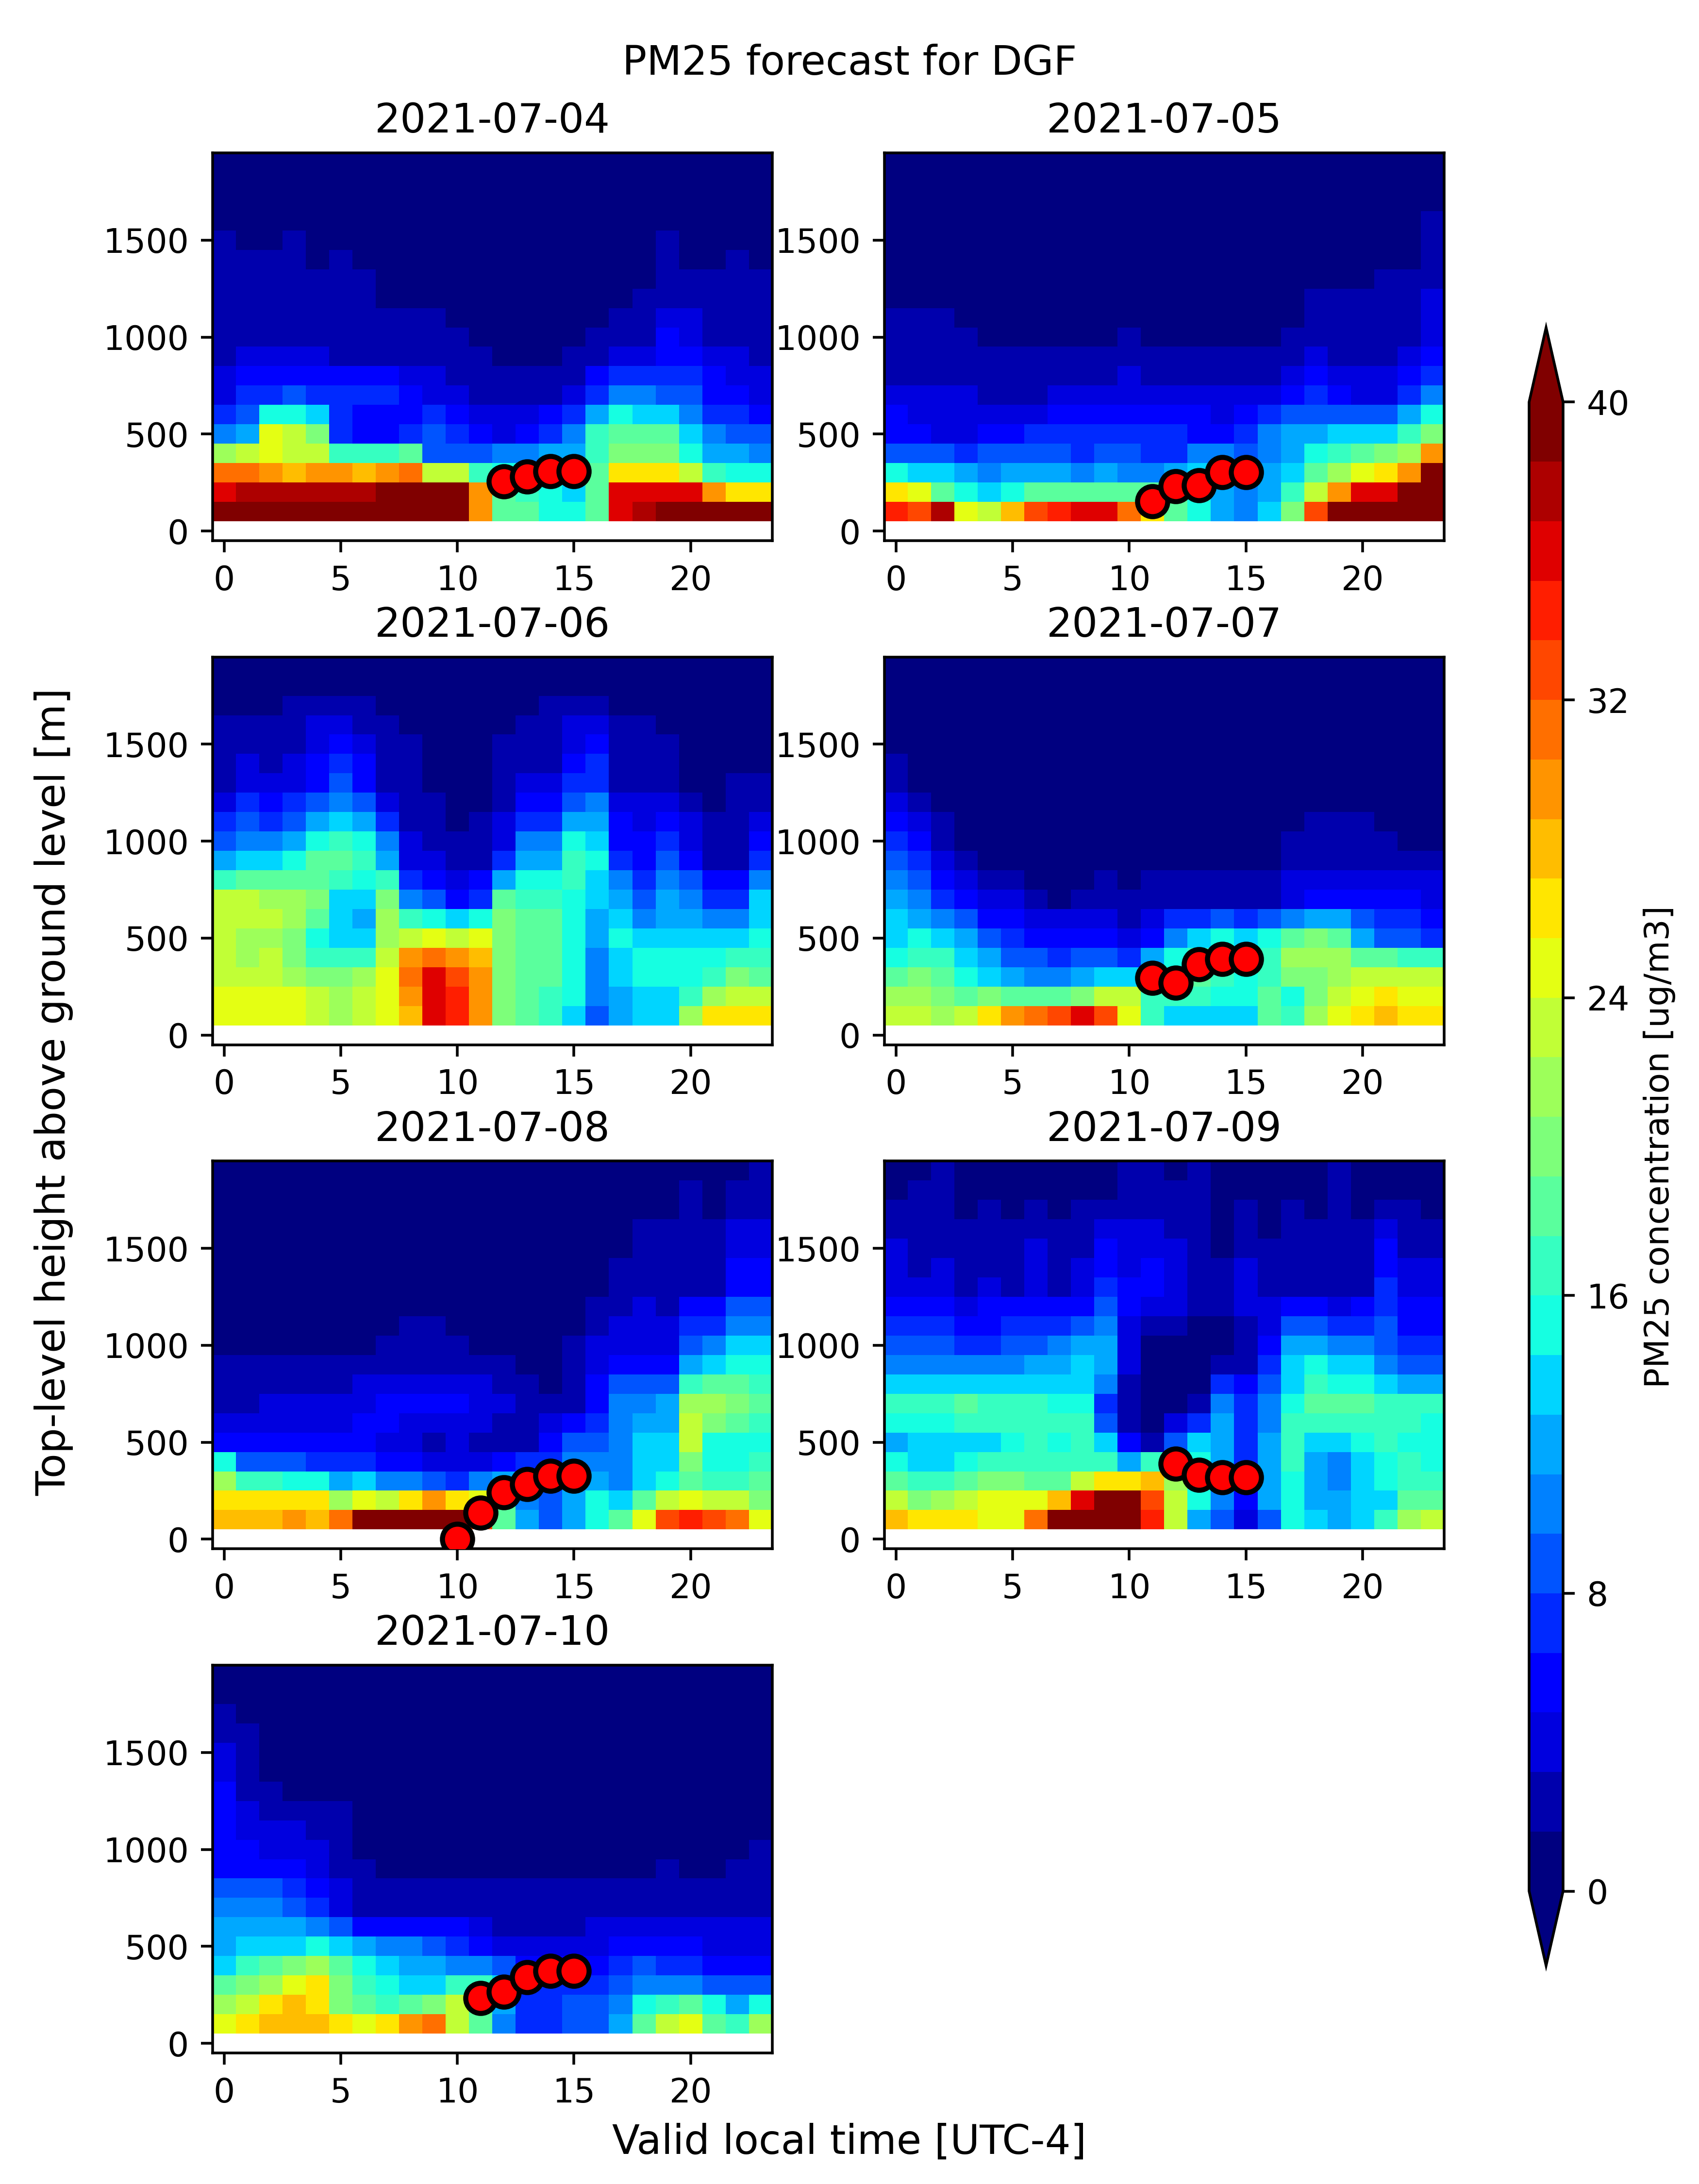
\includegraphics[width=\linewidth]{Figure_7.a.png}
    \end{minipage}
    \hfill
    \begin{minipage}{0.4955\textwidth}
        \centering
        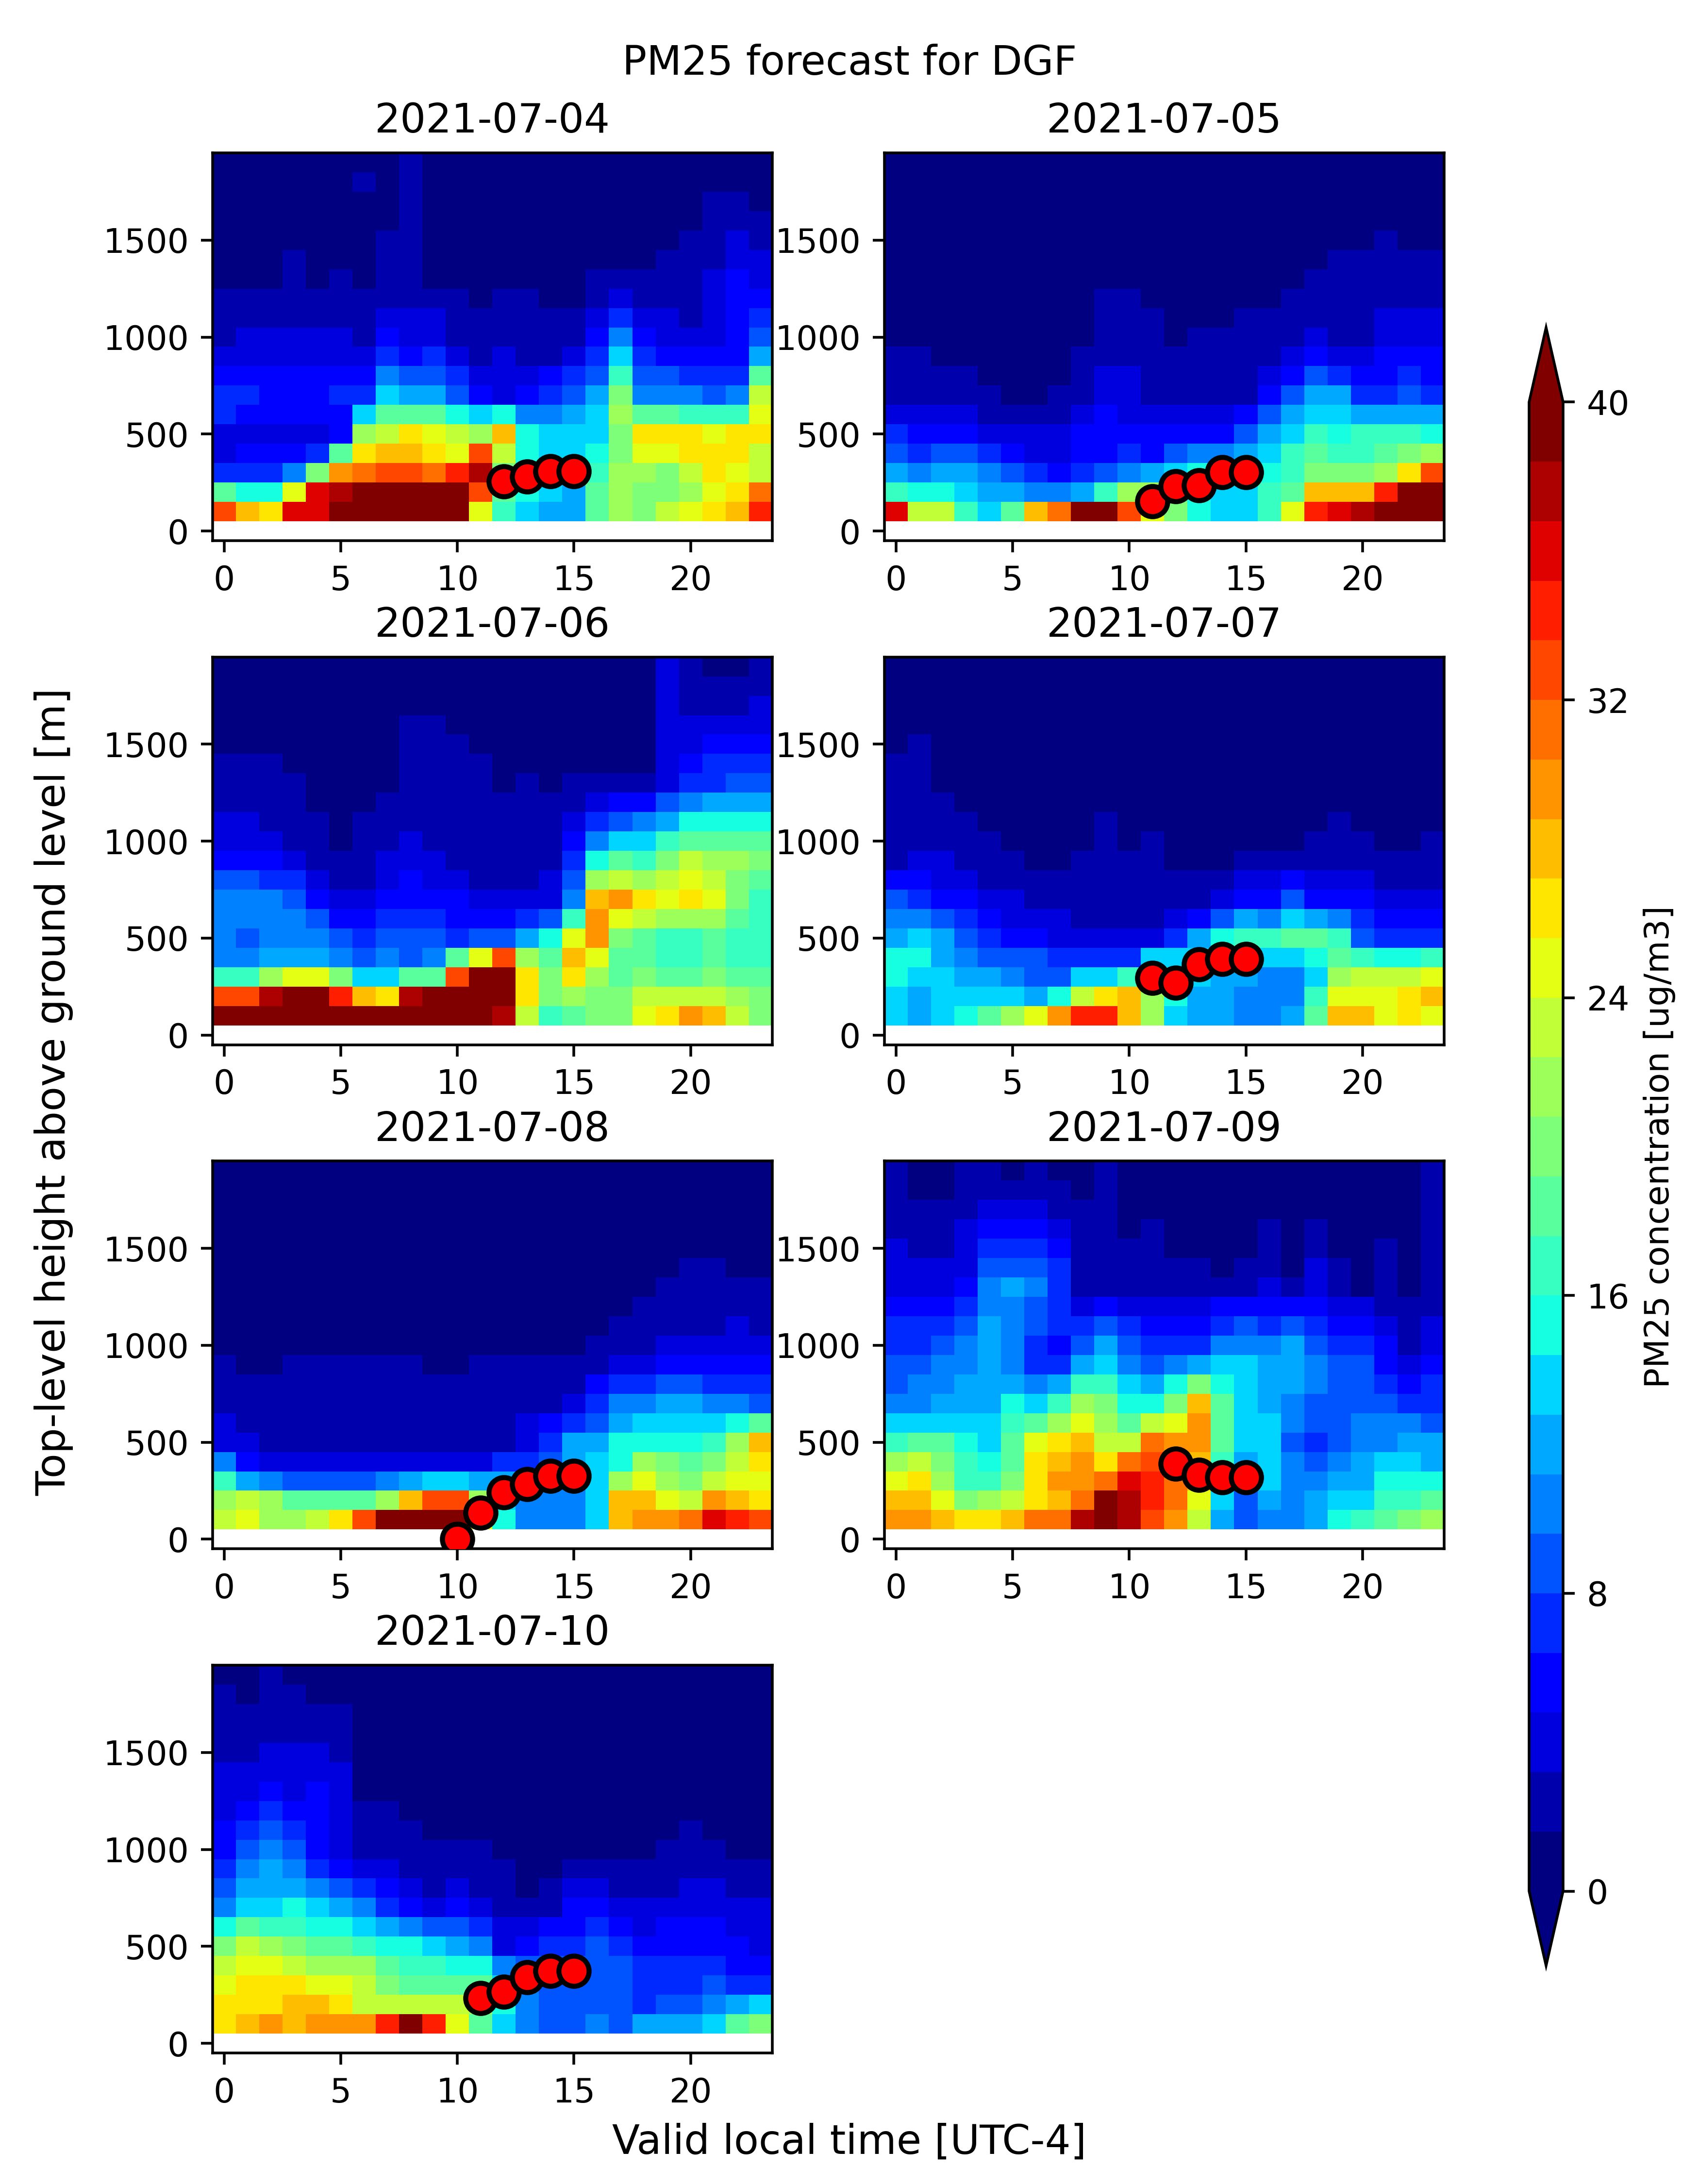
\includegraphics[width=\linewidth]{Figure_7.b.png}
    \end{minipage}
	\textbf{Figure 7} Daily Hovmoller vertical diagrams of PM25 concentrations (colormap), intended to represent the simulated PBLH (planetary boundary layer height) at the closest point to the observed values (red scatterplots) obtained from the Universidad de Chile's Geophysics Department nephobasimeter between 10:00 adn 16:00 local time (UTC-4).
\end{figure}


\section{Conclusions}
\label{conclusions}

Lorem ipsum
\section{Annex}
\label{annex}

\begin{figure}[htbp]
    \centering
    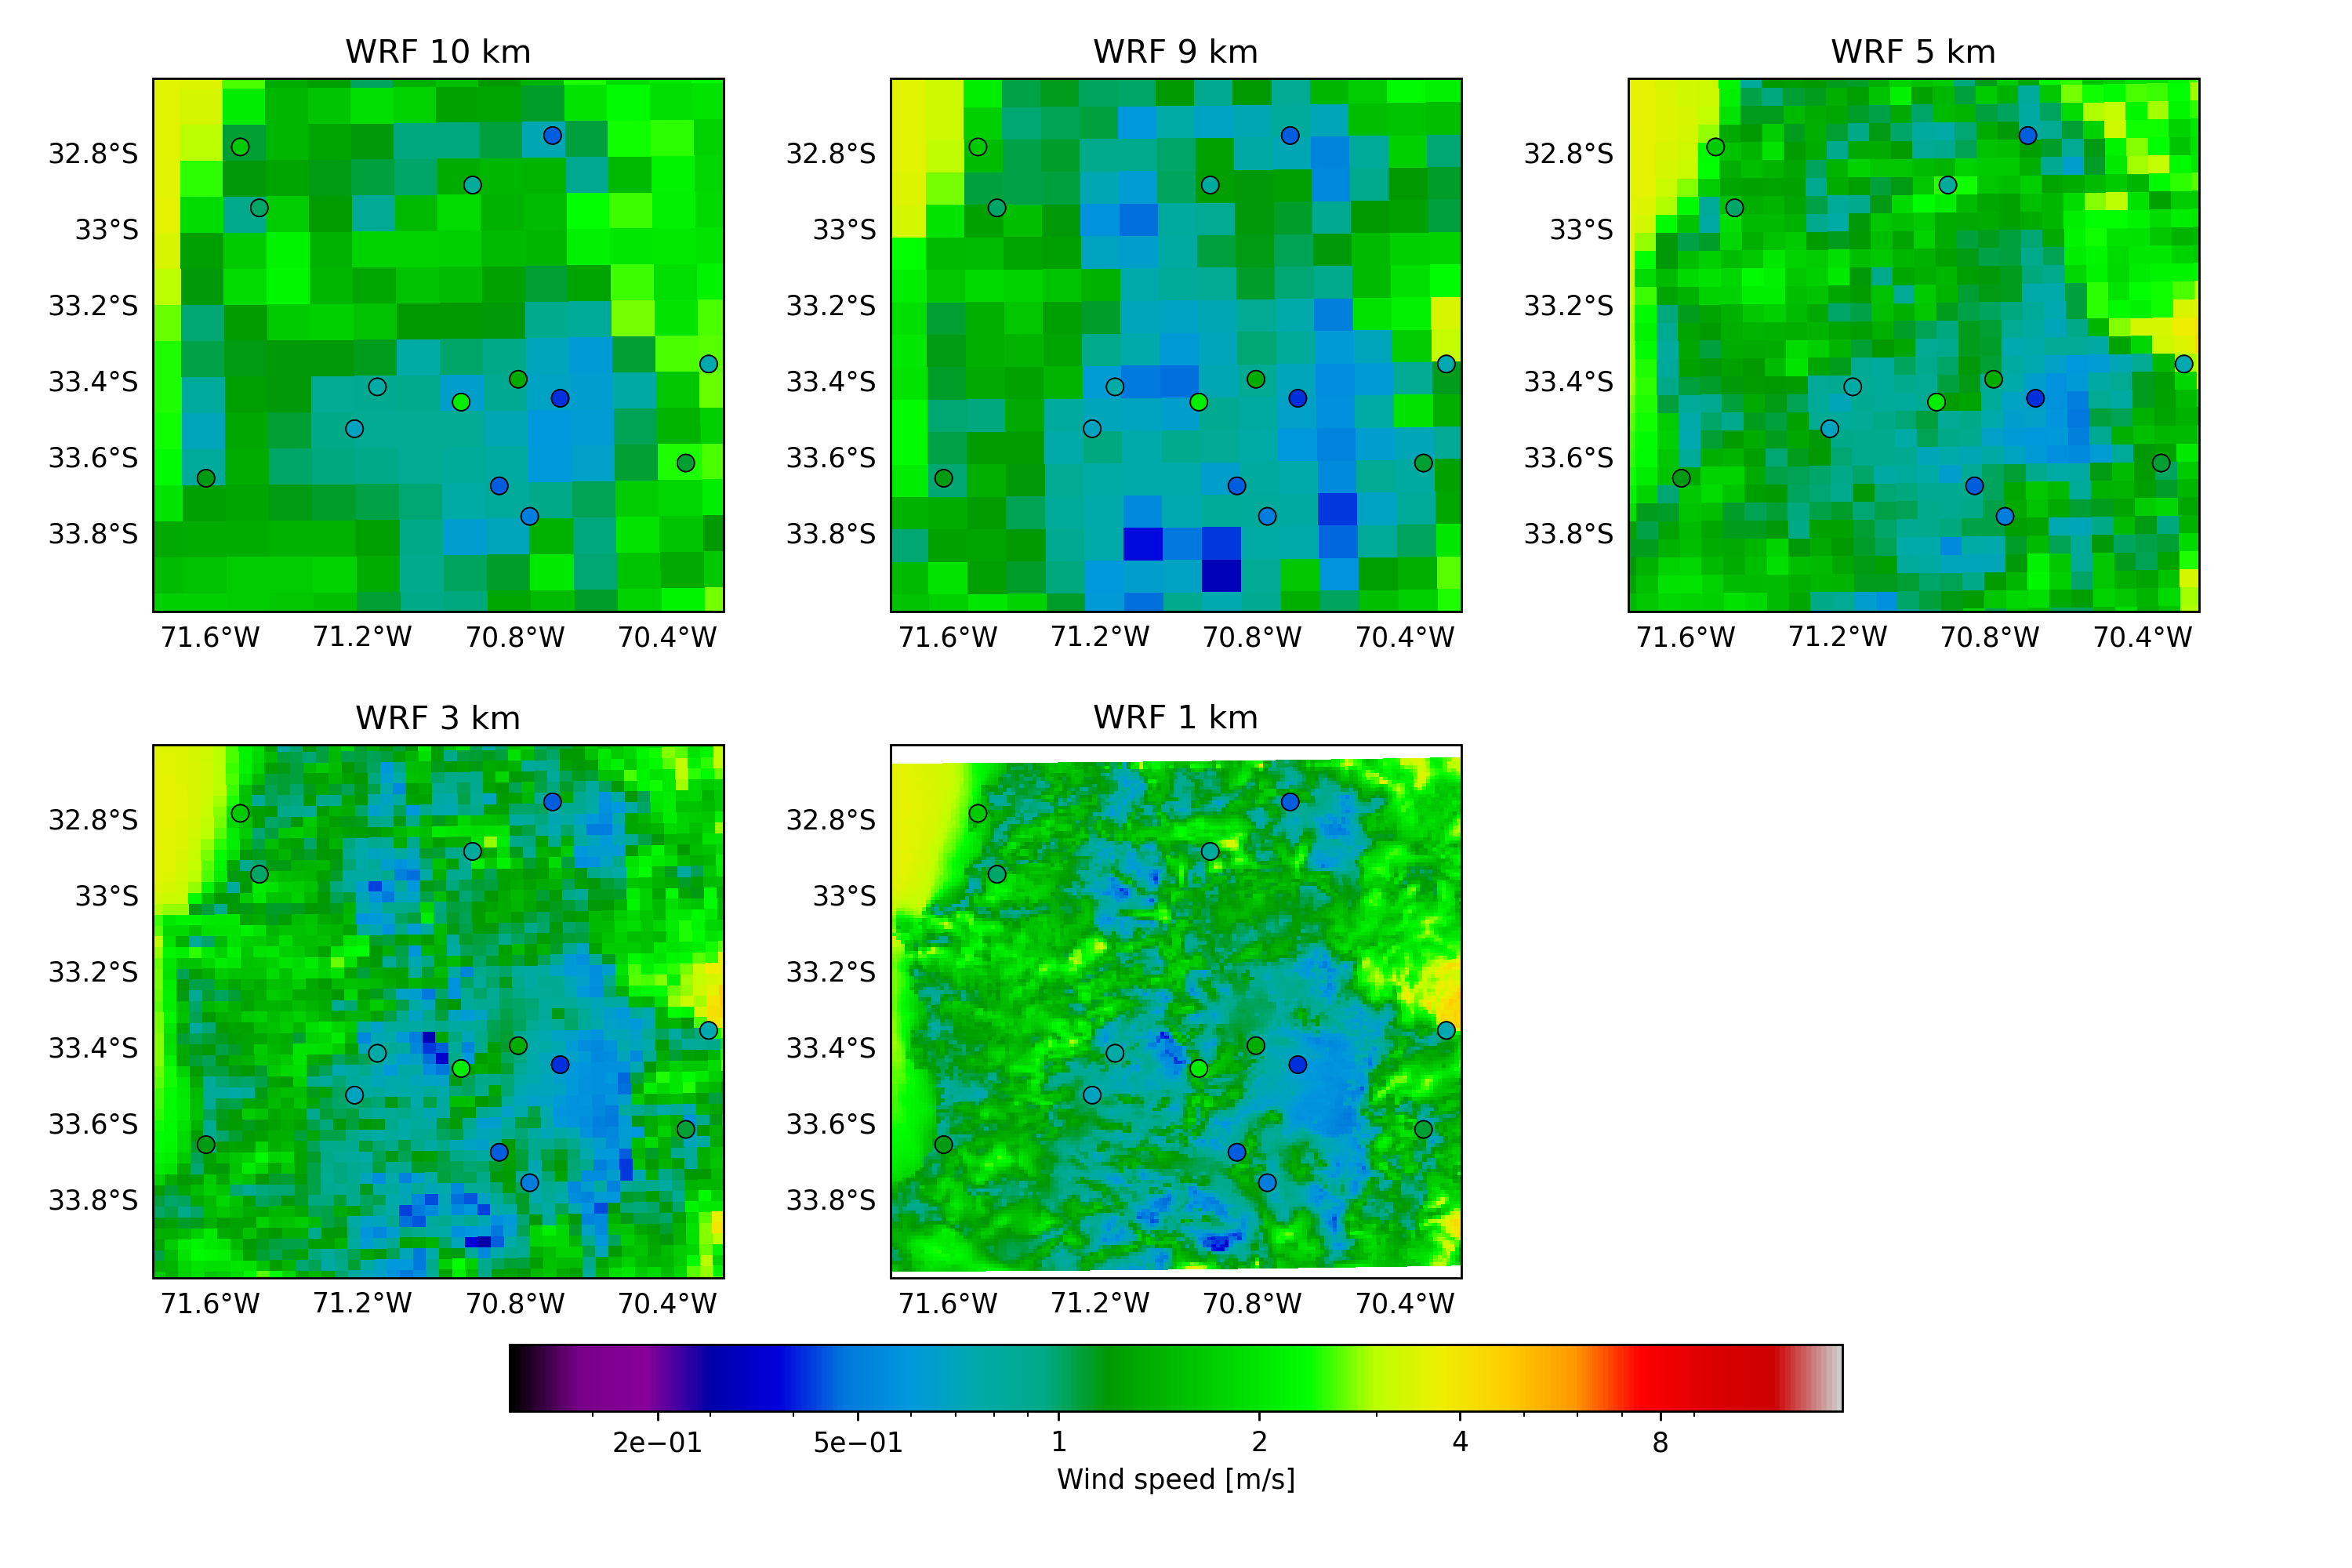
\includegraphics[width=\linewidth,height=8cm]{Annex_3.a.png}
    \textbf{Annex 3.a} Temporal standard deviation of configuration C for 10-meter wind speed fields across Central Chile (colormap), compared to the temporal standard deviation of the station observations for the same period (scatterplots). The corresponding leadtime is of 24 hours
\end{figure}

\begin{figure}[htbp]
    \centering
    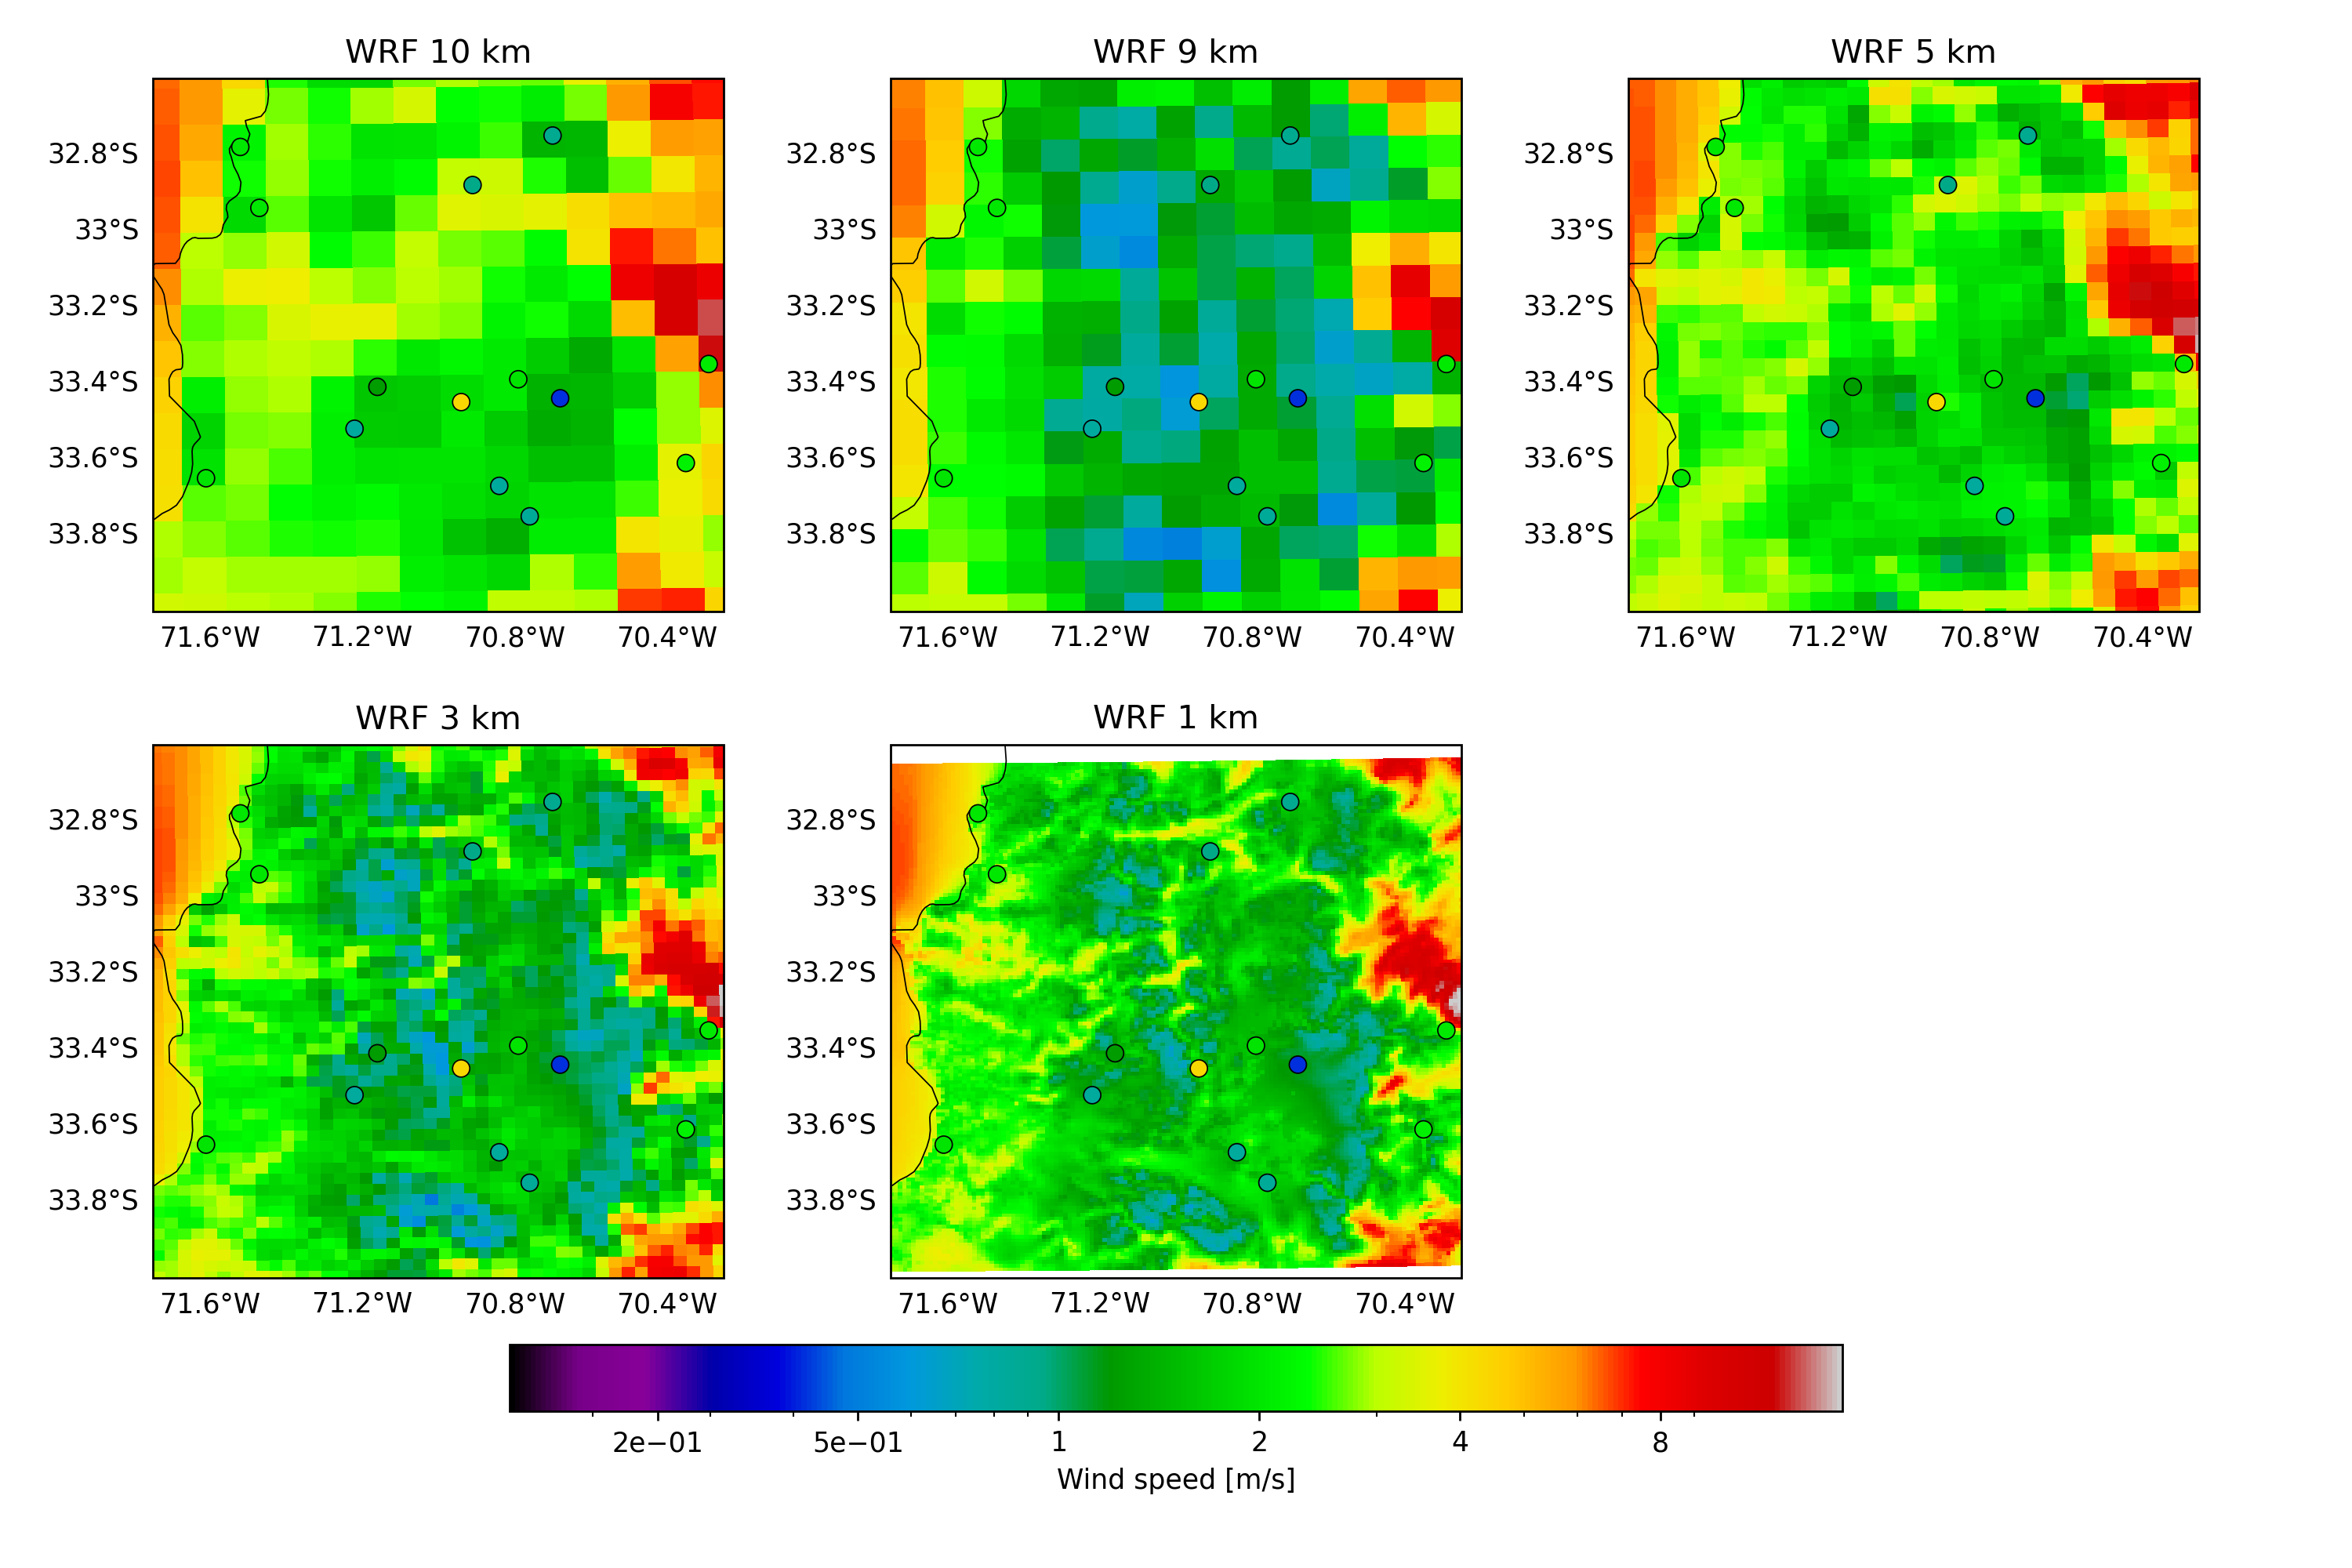
\includegraphics[width=\linewidth,height=8cm]{Annex_3.b.png}
    \textbf{Annex 3.b} Temporal mean of configuration C for 10-meter wind speed fields across Central Chile (colormap), compared to the temporal mean of the station observations for the same period (scatterplots).  The corresponding leadtime is of 96 hours
\end{figure}

\begin{figure}[htbp]
    \centering
    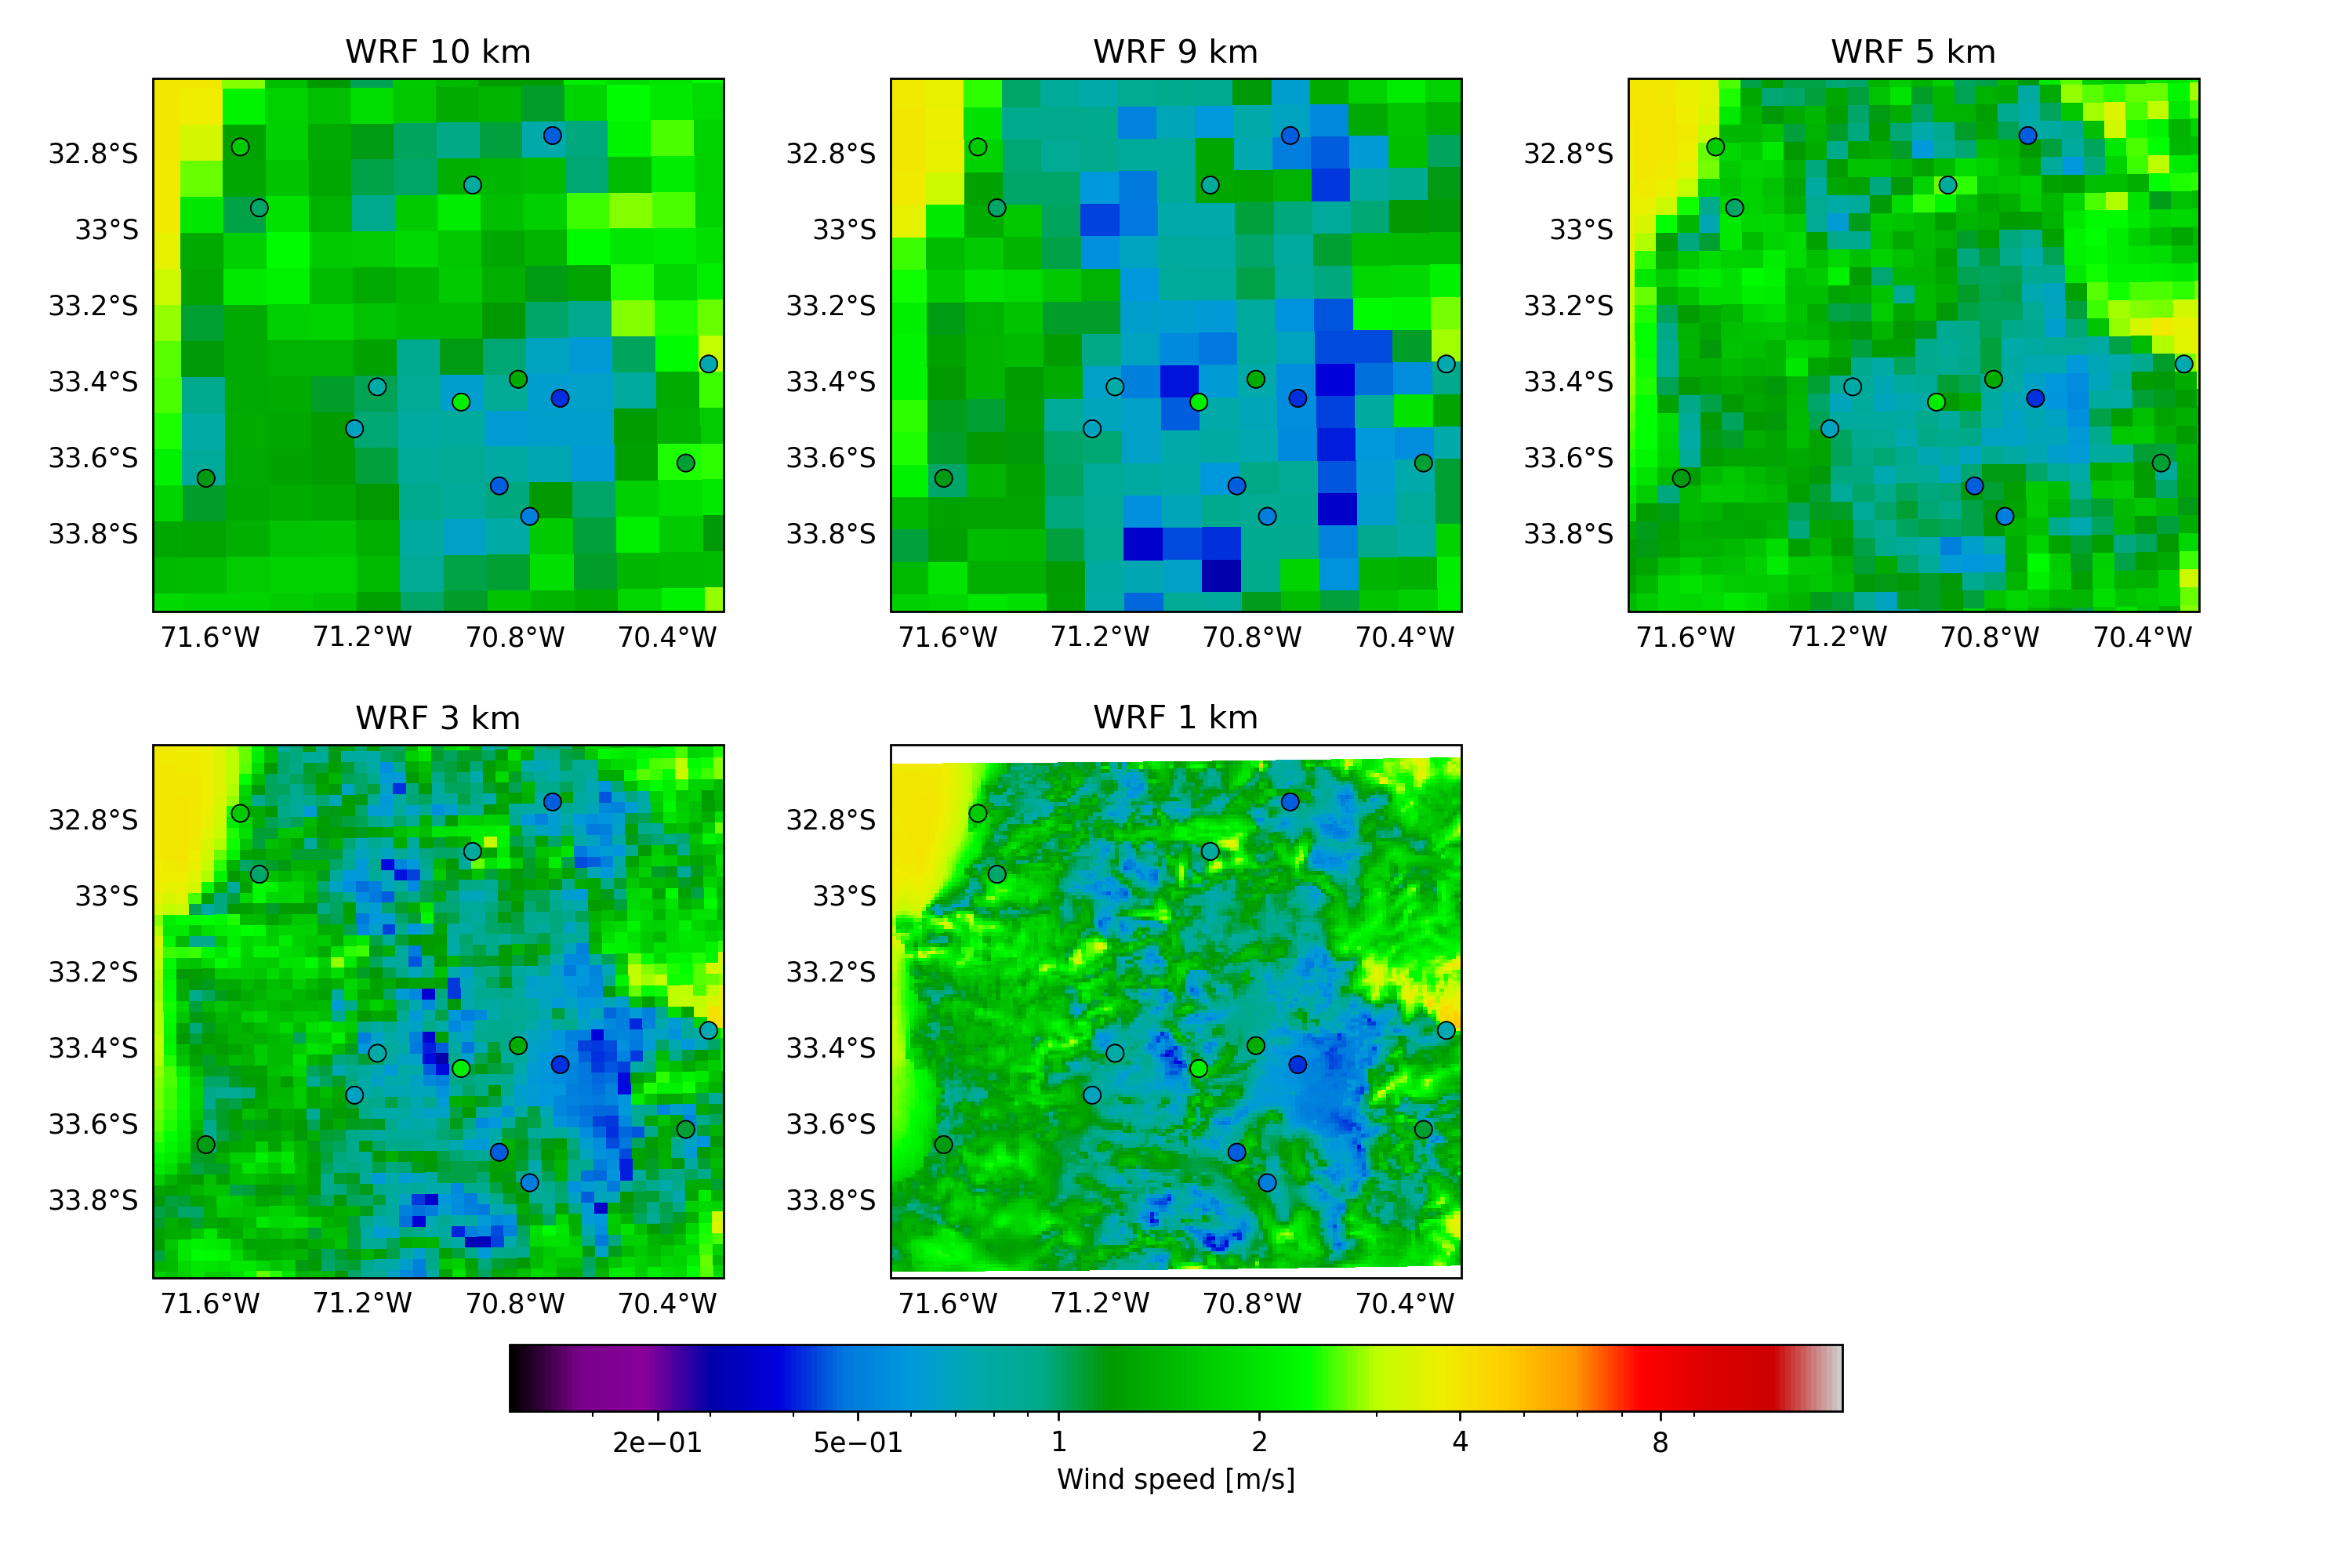
\includegraphics[width=\linewidth,height=8cm]{Annex_3.c.png}
    \textbf{Annex 3.c} Temporal standard deviation of configuration C for 10-meter wind speed fields across Central Chile (colormap), compared to the temporal standard deviation of the station observations for the same period (scatterplots).  The corresponding leadtime is of 96 hours
\end{figure}

\begin{figure}[htbp]
    \centering
    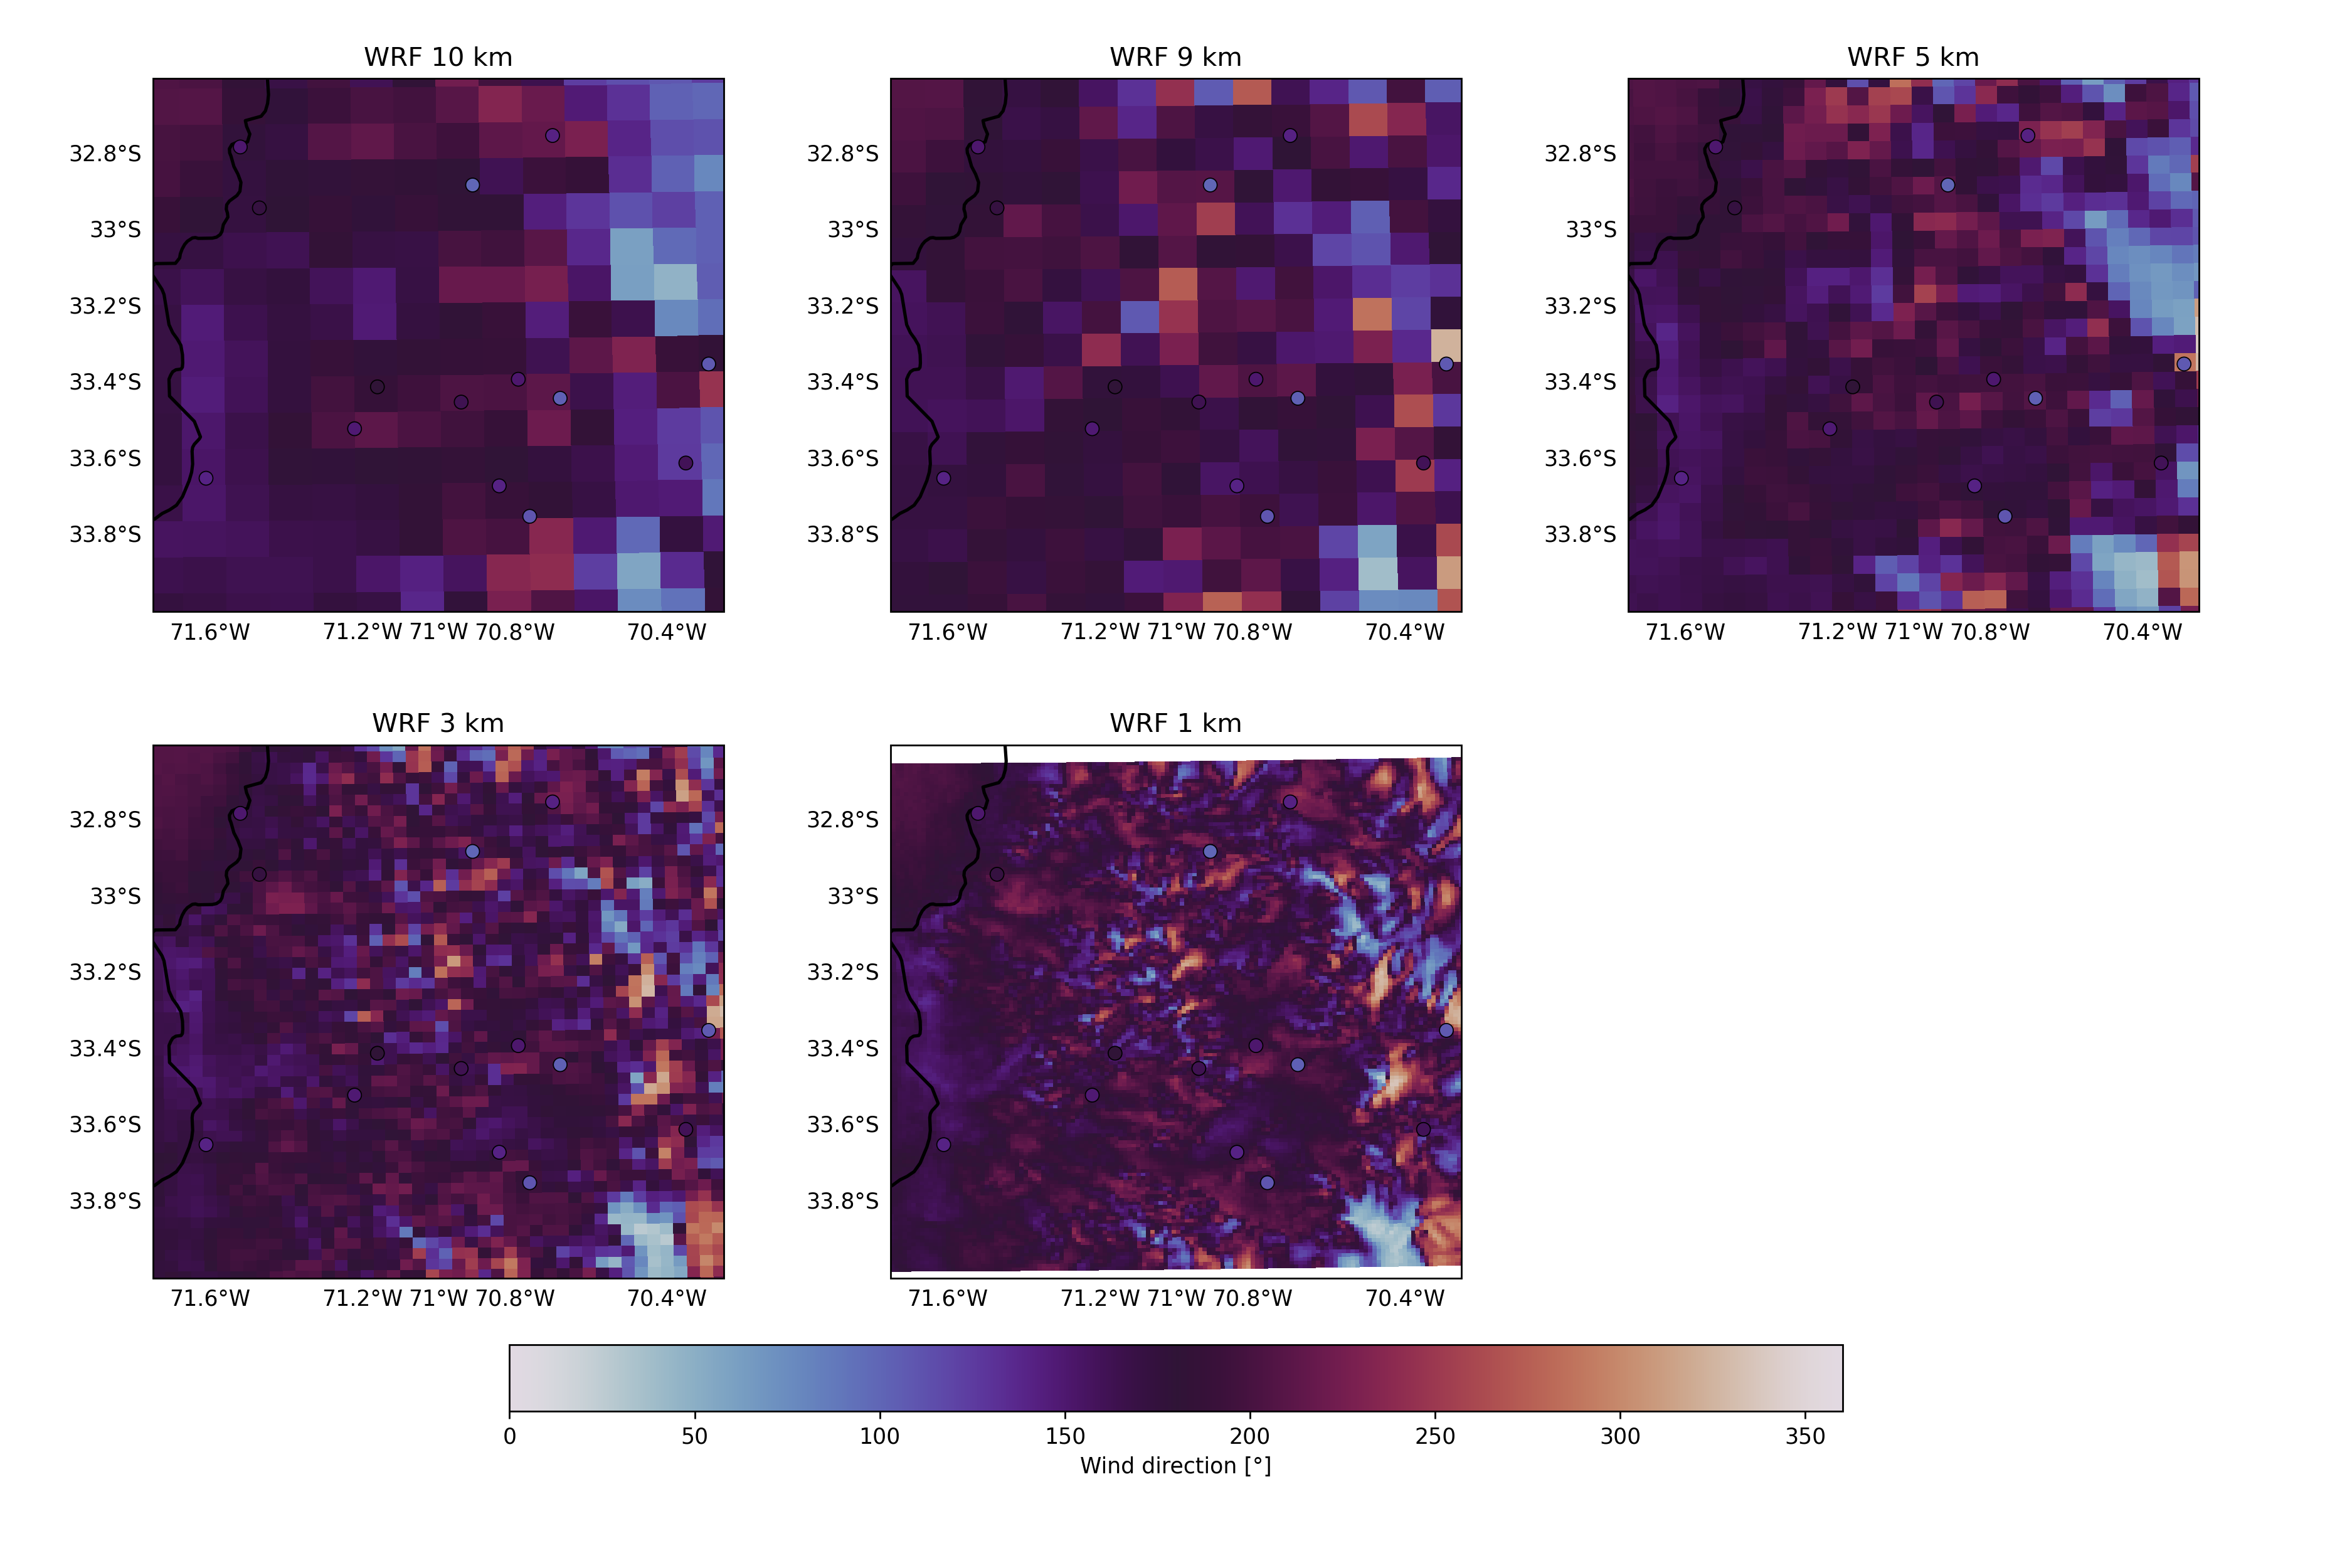
\includegraphics[width=\linewidth,height=8cm]{Annex_3.d.png}
    \textbf{Annex 3.d} Temporal mean of configuration C for 10-meter wind direction fields across Central Chile (colormap), compared to the temporal mean of the station observations for the same period (scatterplots).  The corresponding leadtime is of 96 hours
\end{figure}

\begin{figure}[htbp]
    \centering
    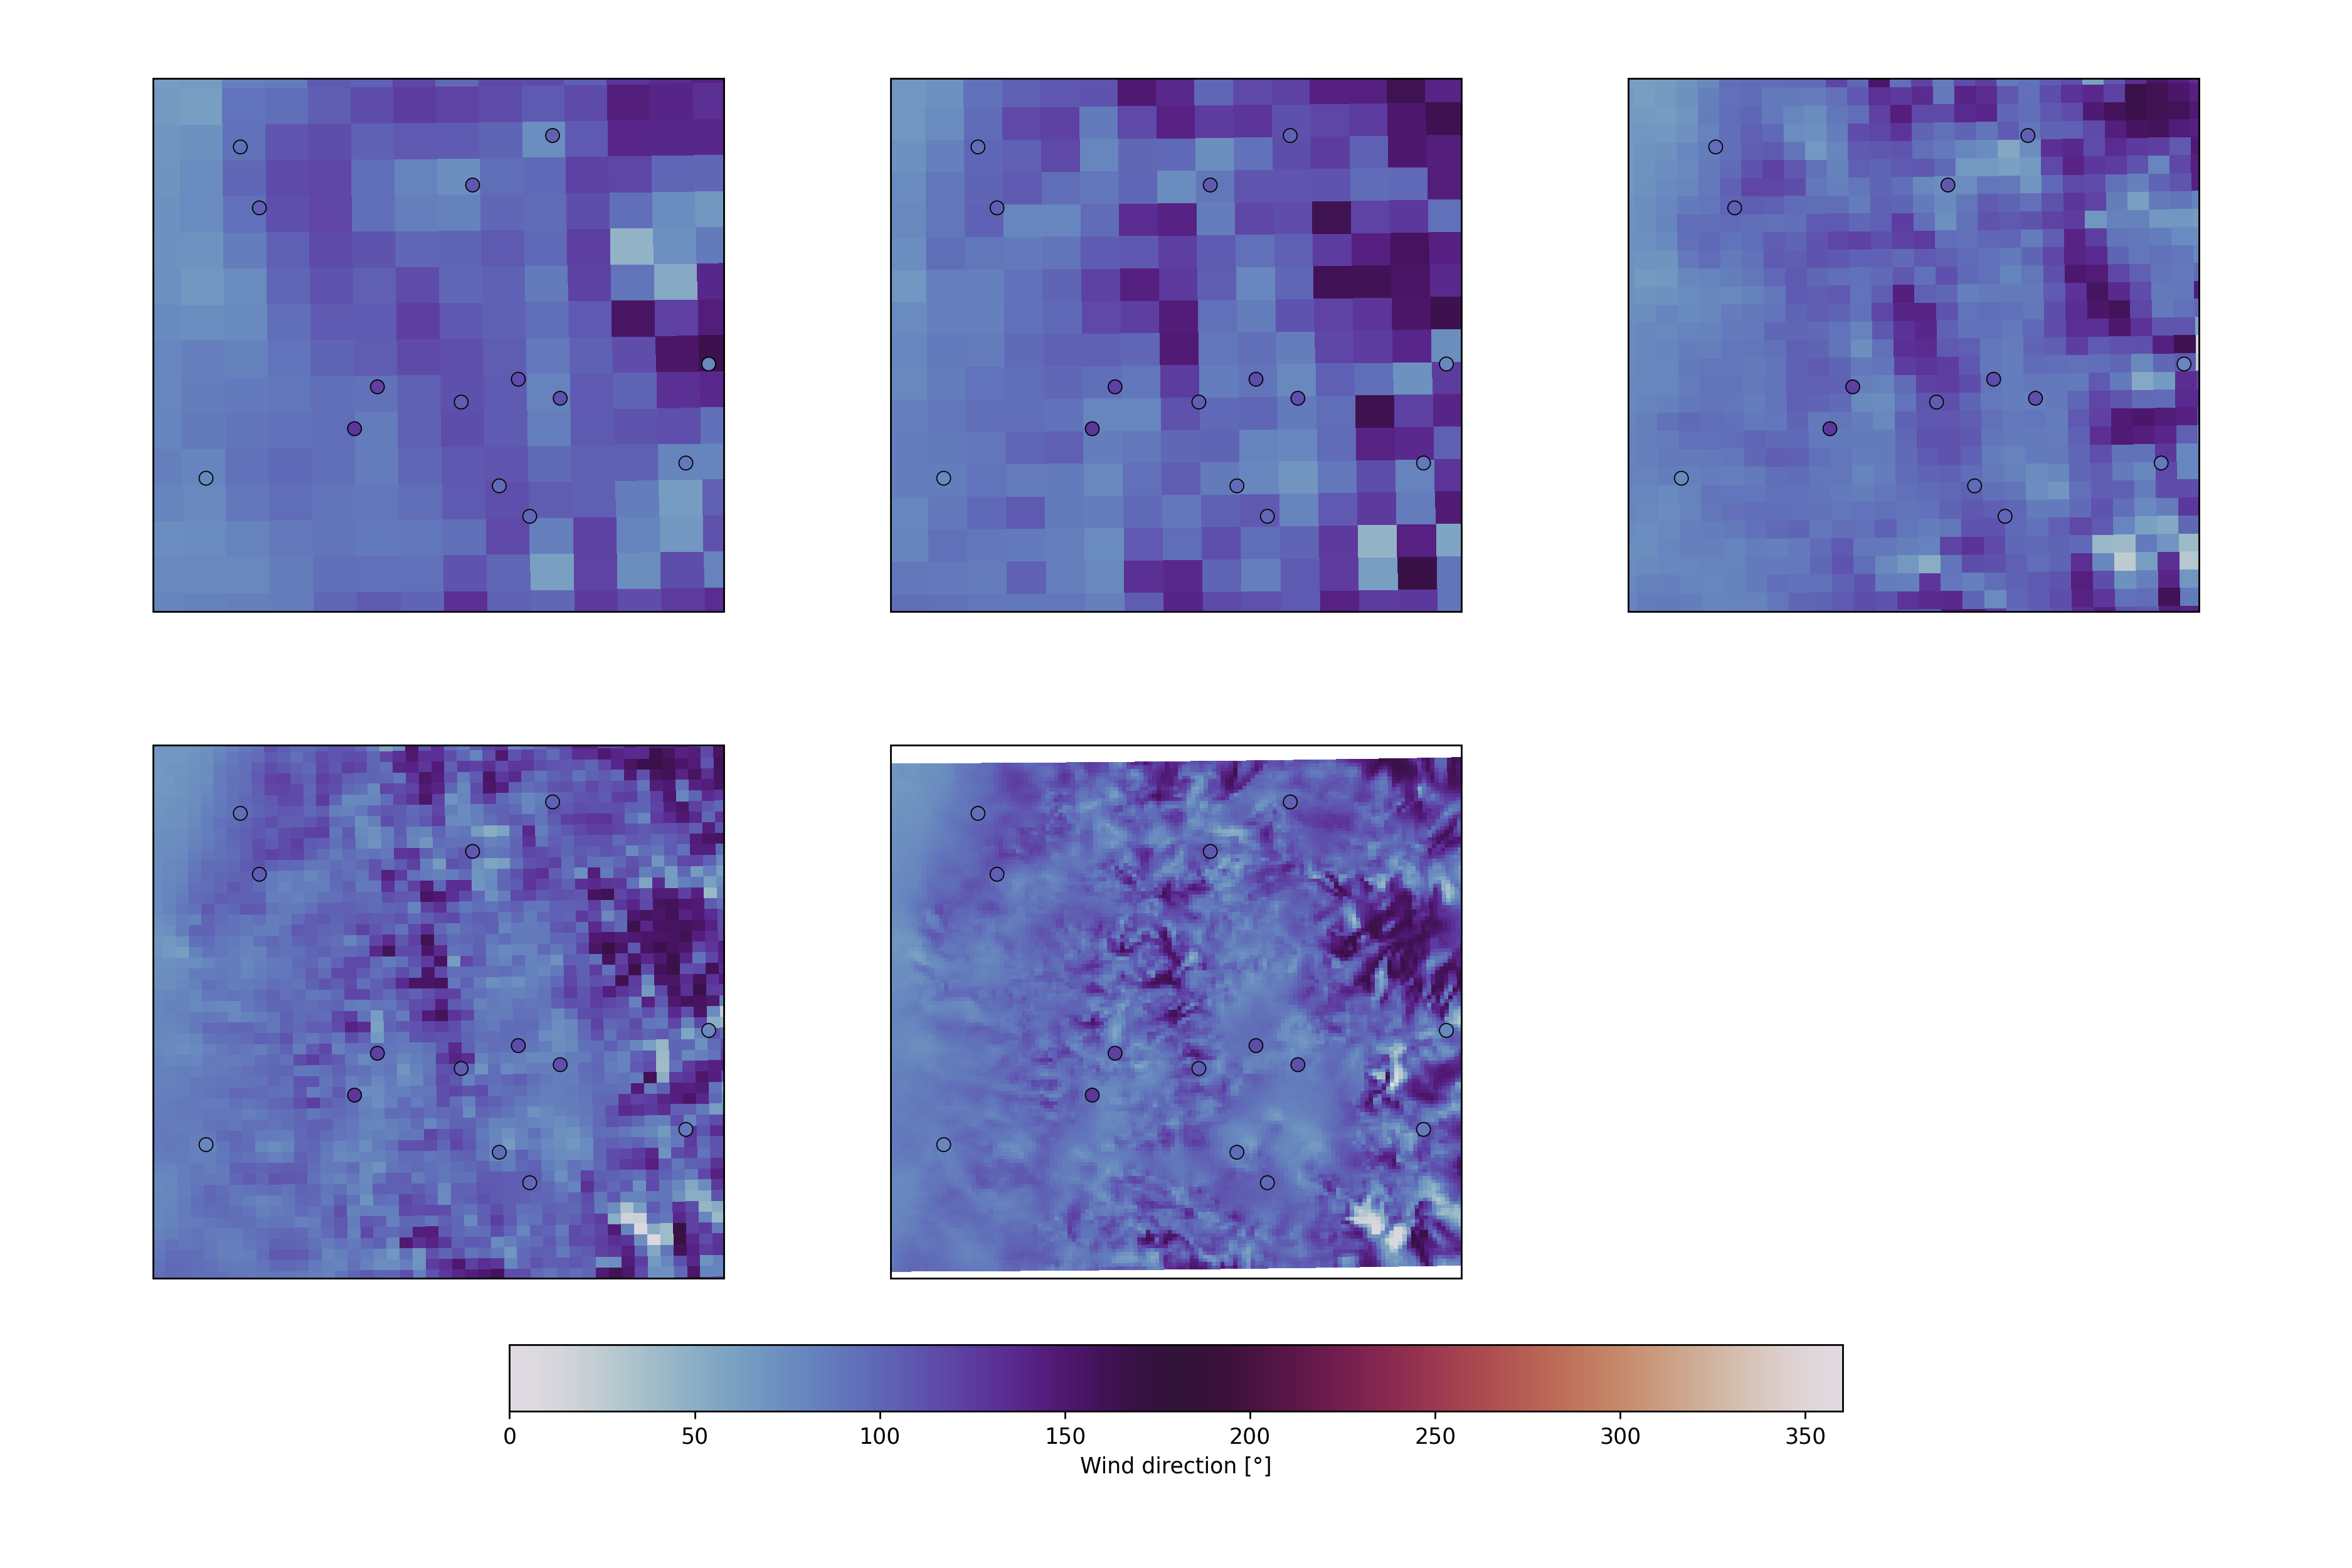
\includegraphics[width=\linewidth,height=8cm]{Annex_3.e.png}
    \textbf{Annex 3.e} Temporal standard deviation of configuration C for 10-meter wind direction fields across Central Chile (colormap), compared to the temporal standard deviation of the station observations for the same period (scatterplots).  The corresponding leadtime is of 96 hours 
\end{figure}

\begin{figure}[htbp]
    \centering
    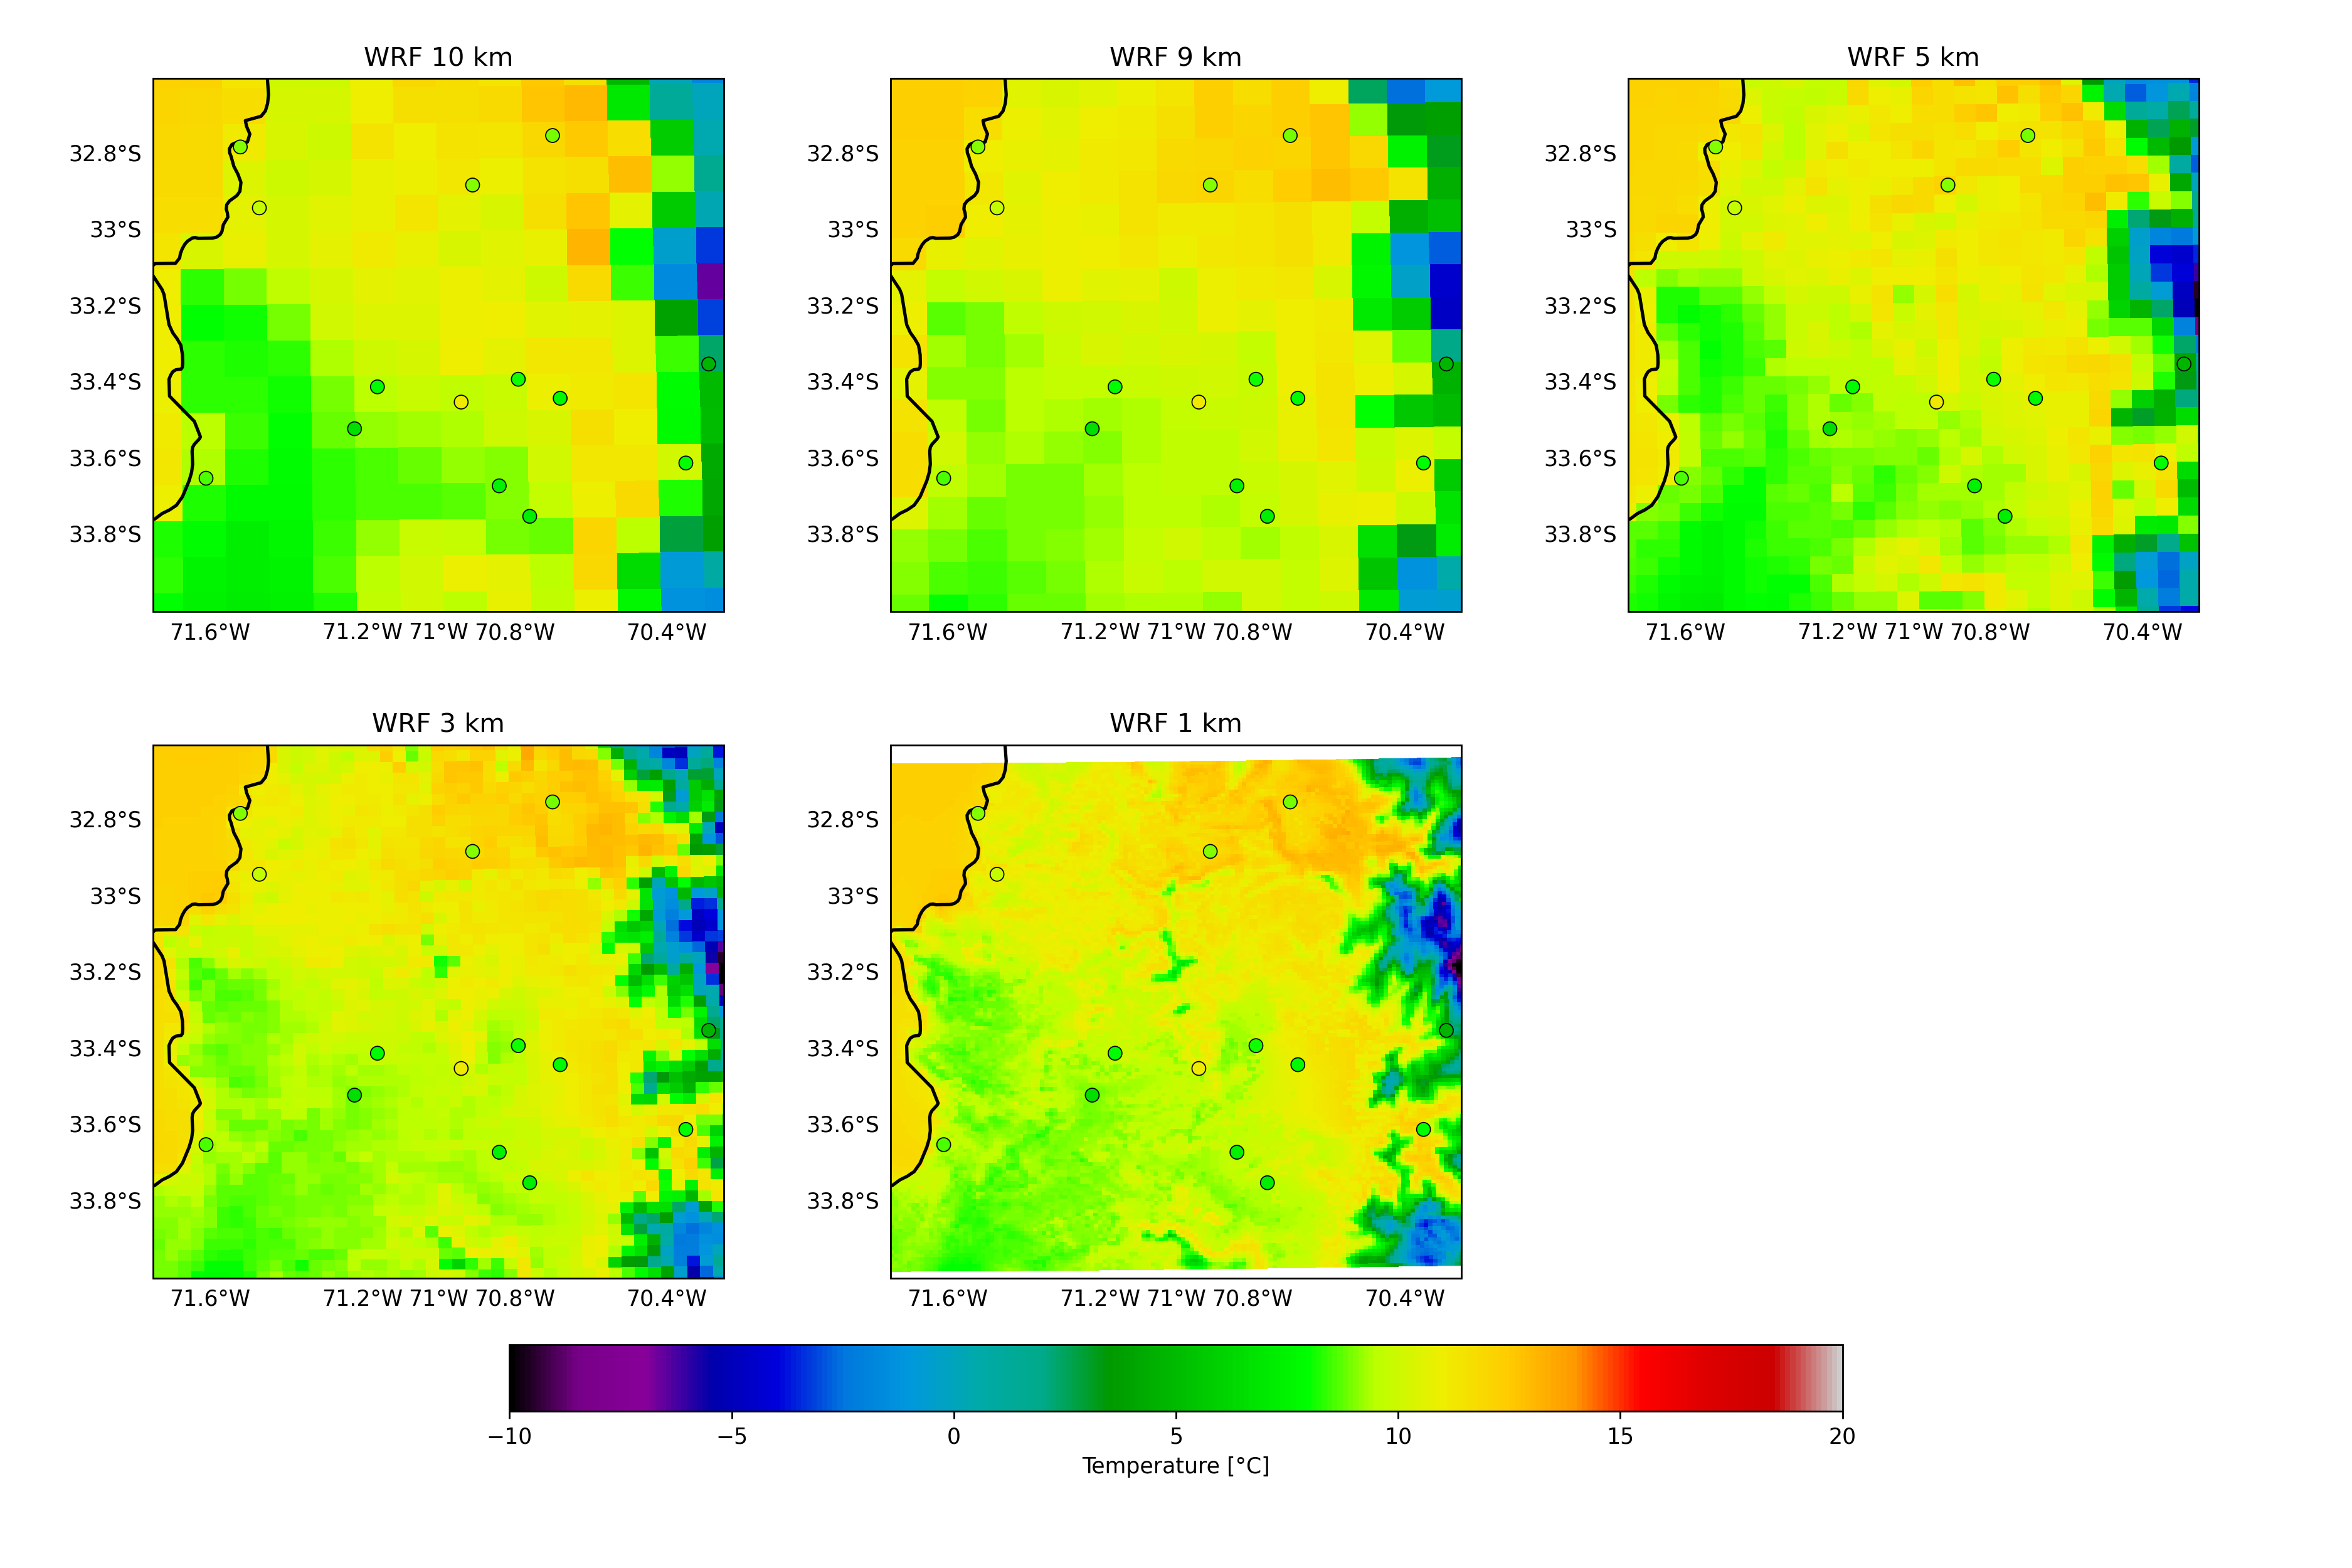
\includegraphics[width=\linewidth,height=8cm]{Annex_3.f.png}
    \textbf{Annex 3.f} Temporal mean of configuration C for 2-meter temperature fields across Central Chile (colormap), compared to the temporal mean of the station observations for the same period (scatterplots).  The corresponding leadtime is of 24 hours
\end{figure}

\begin{figure}[htbp]
    \centering
    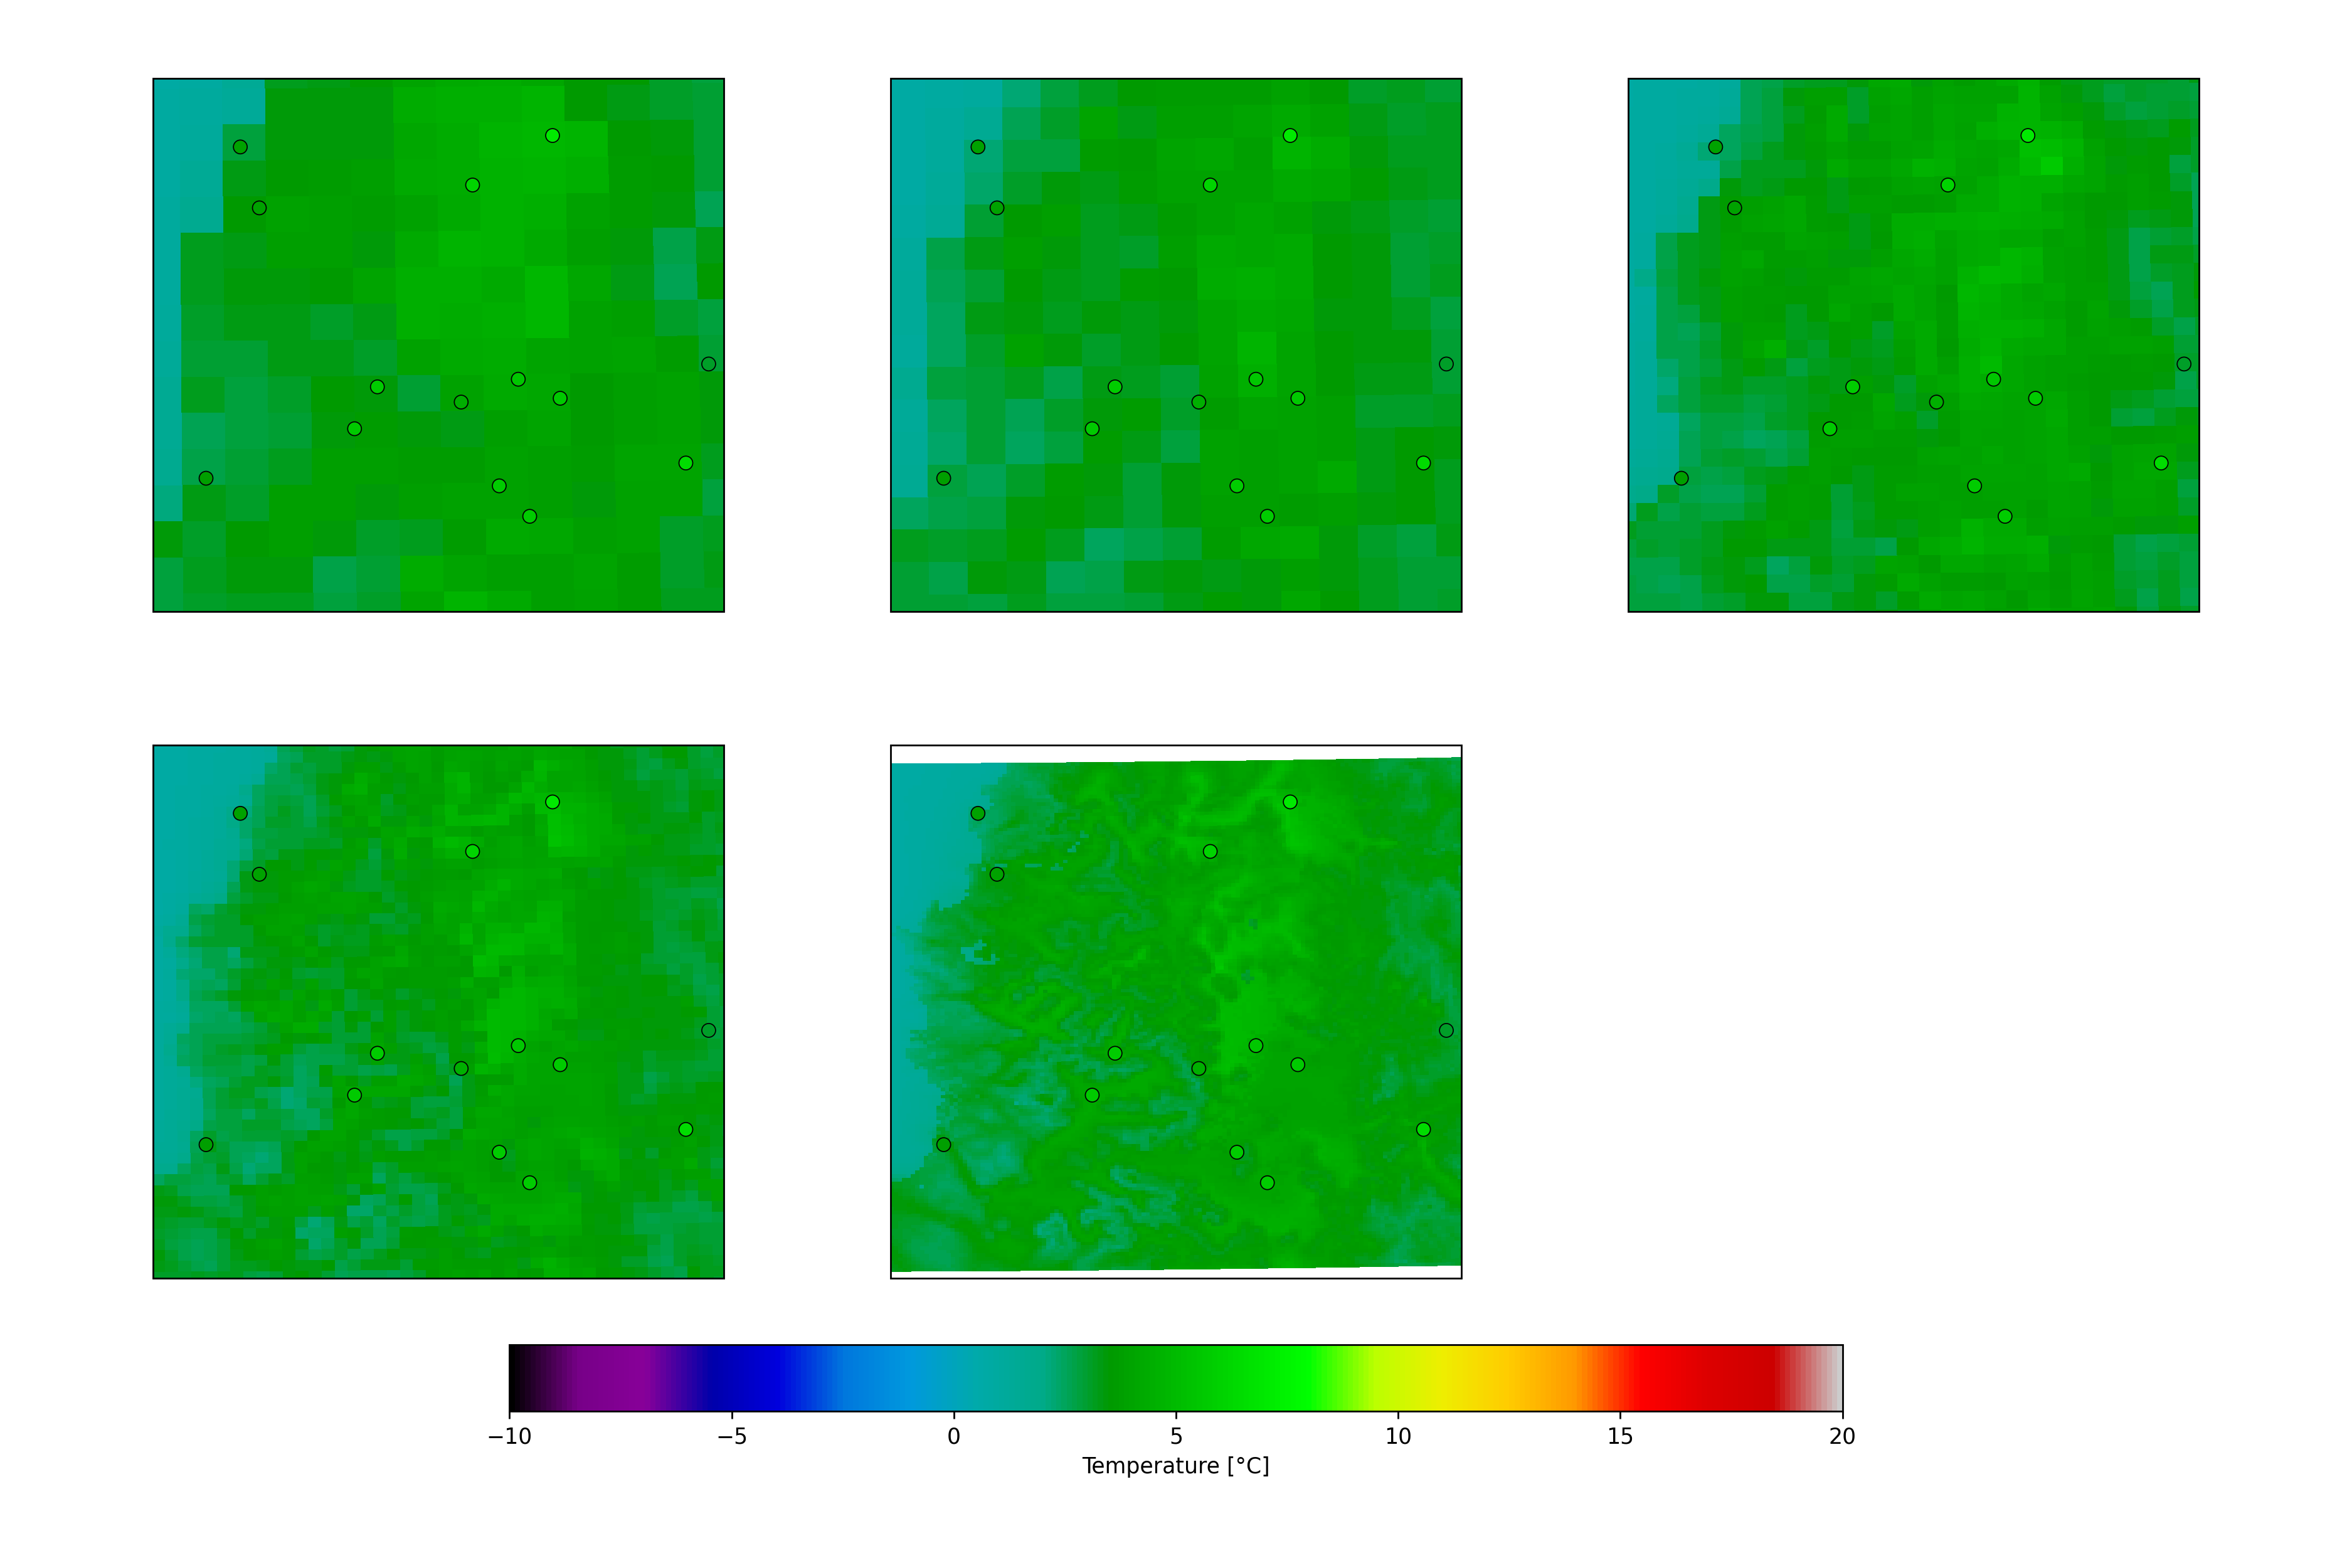
\includegraphics[width=\linewidth,height=8cm]{Annex_3.g.png}
    \textbf{Annex 3.g} Temporal standard deviation of configuration C for 2-meter temperature fields across Central Chile (colormap), compared to the temporal standard deviation of the station observations for the same period (scatterplots).  The corresponding leadtime is of 24 hours
\end{figure}

\begin{figure}[htbp]
    \centering
    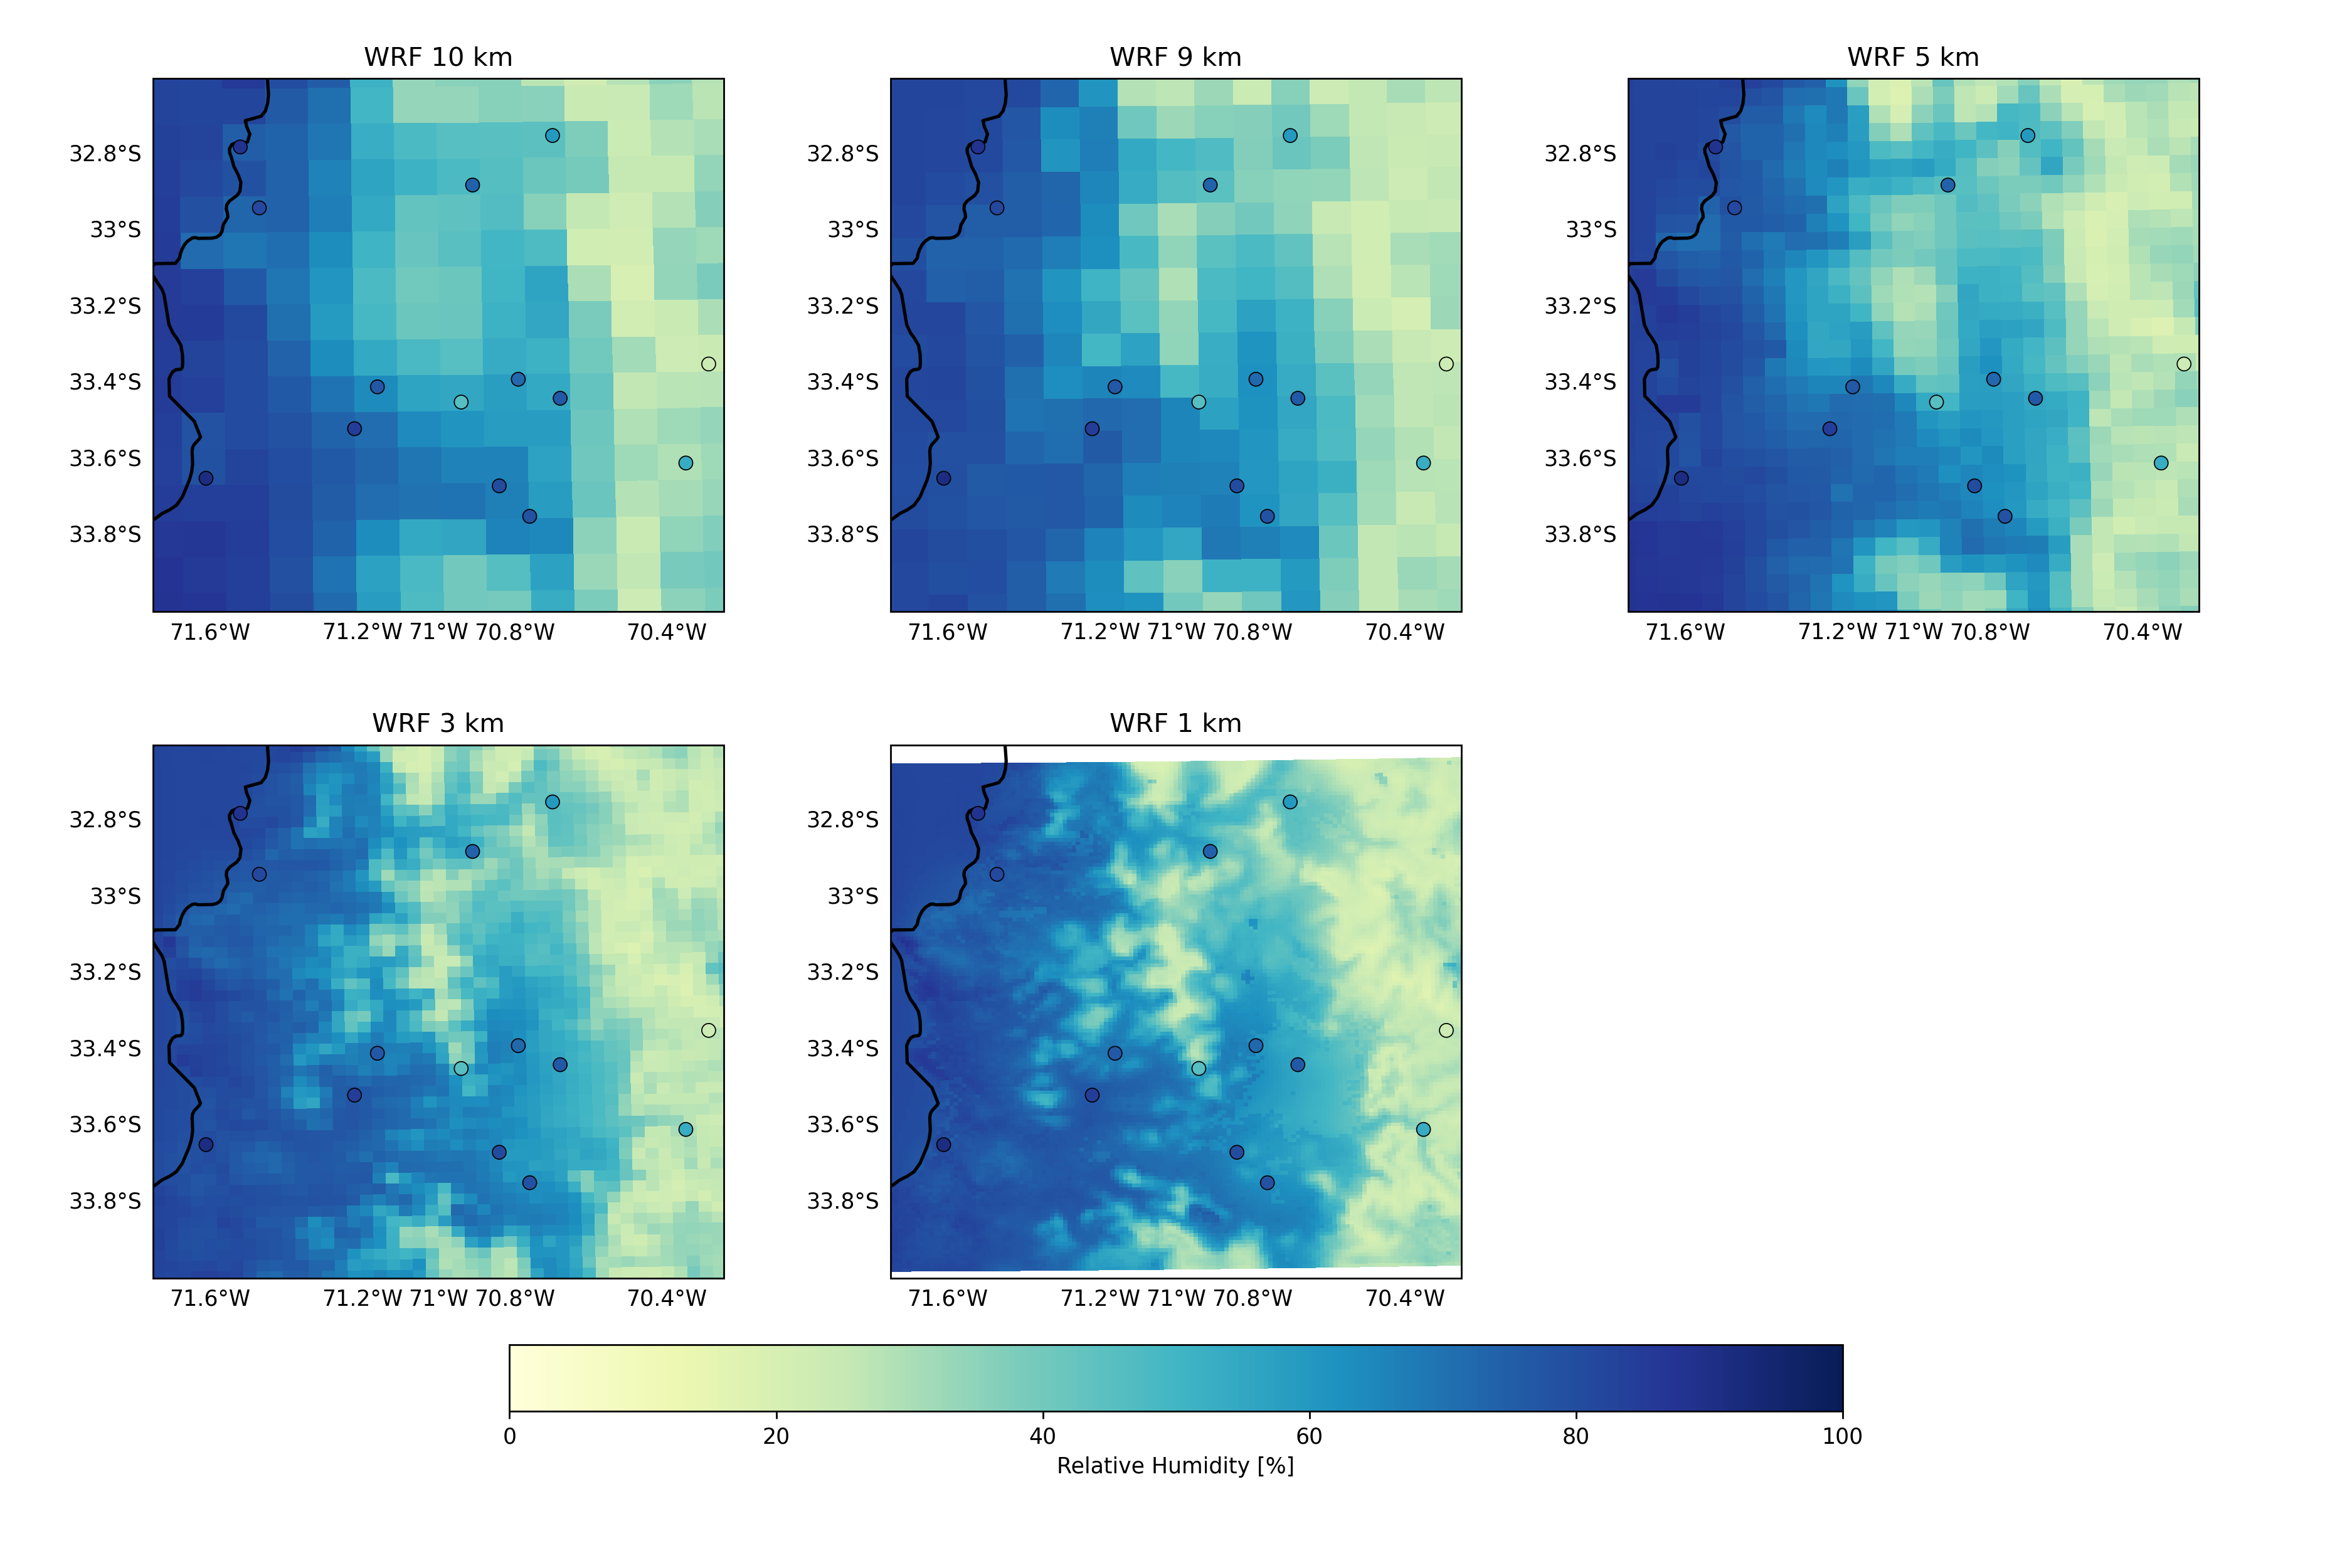
\includegraphics[width=\linewidth,height=8cm]{Annex_3.h.png}
    \textbf{Annex 3.h} Temporal mean of configuration C for 2-meter relative humidity fields across Central Chile (colormap), compared to the temporal mean of the station observations for the same period (scatterplots).  The corresponding leadtime is of 24 hours
\end{figure}

\begin{figure}[htbp]
    \centering
    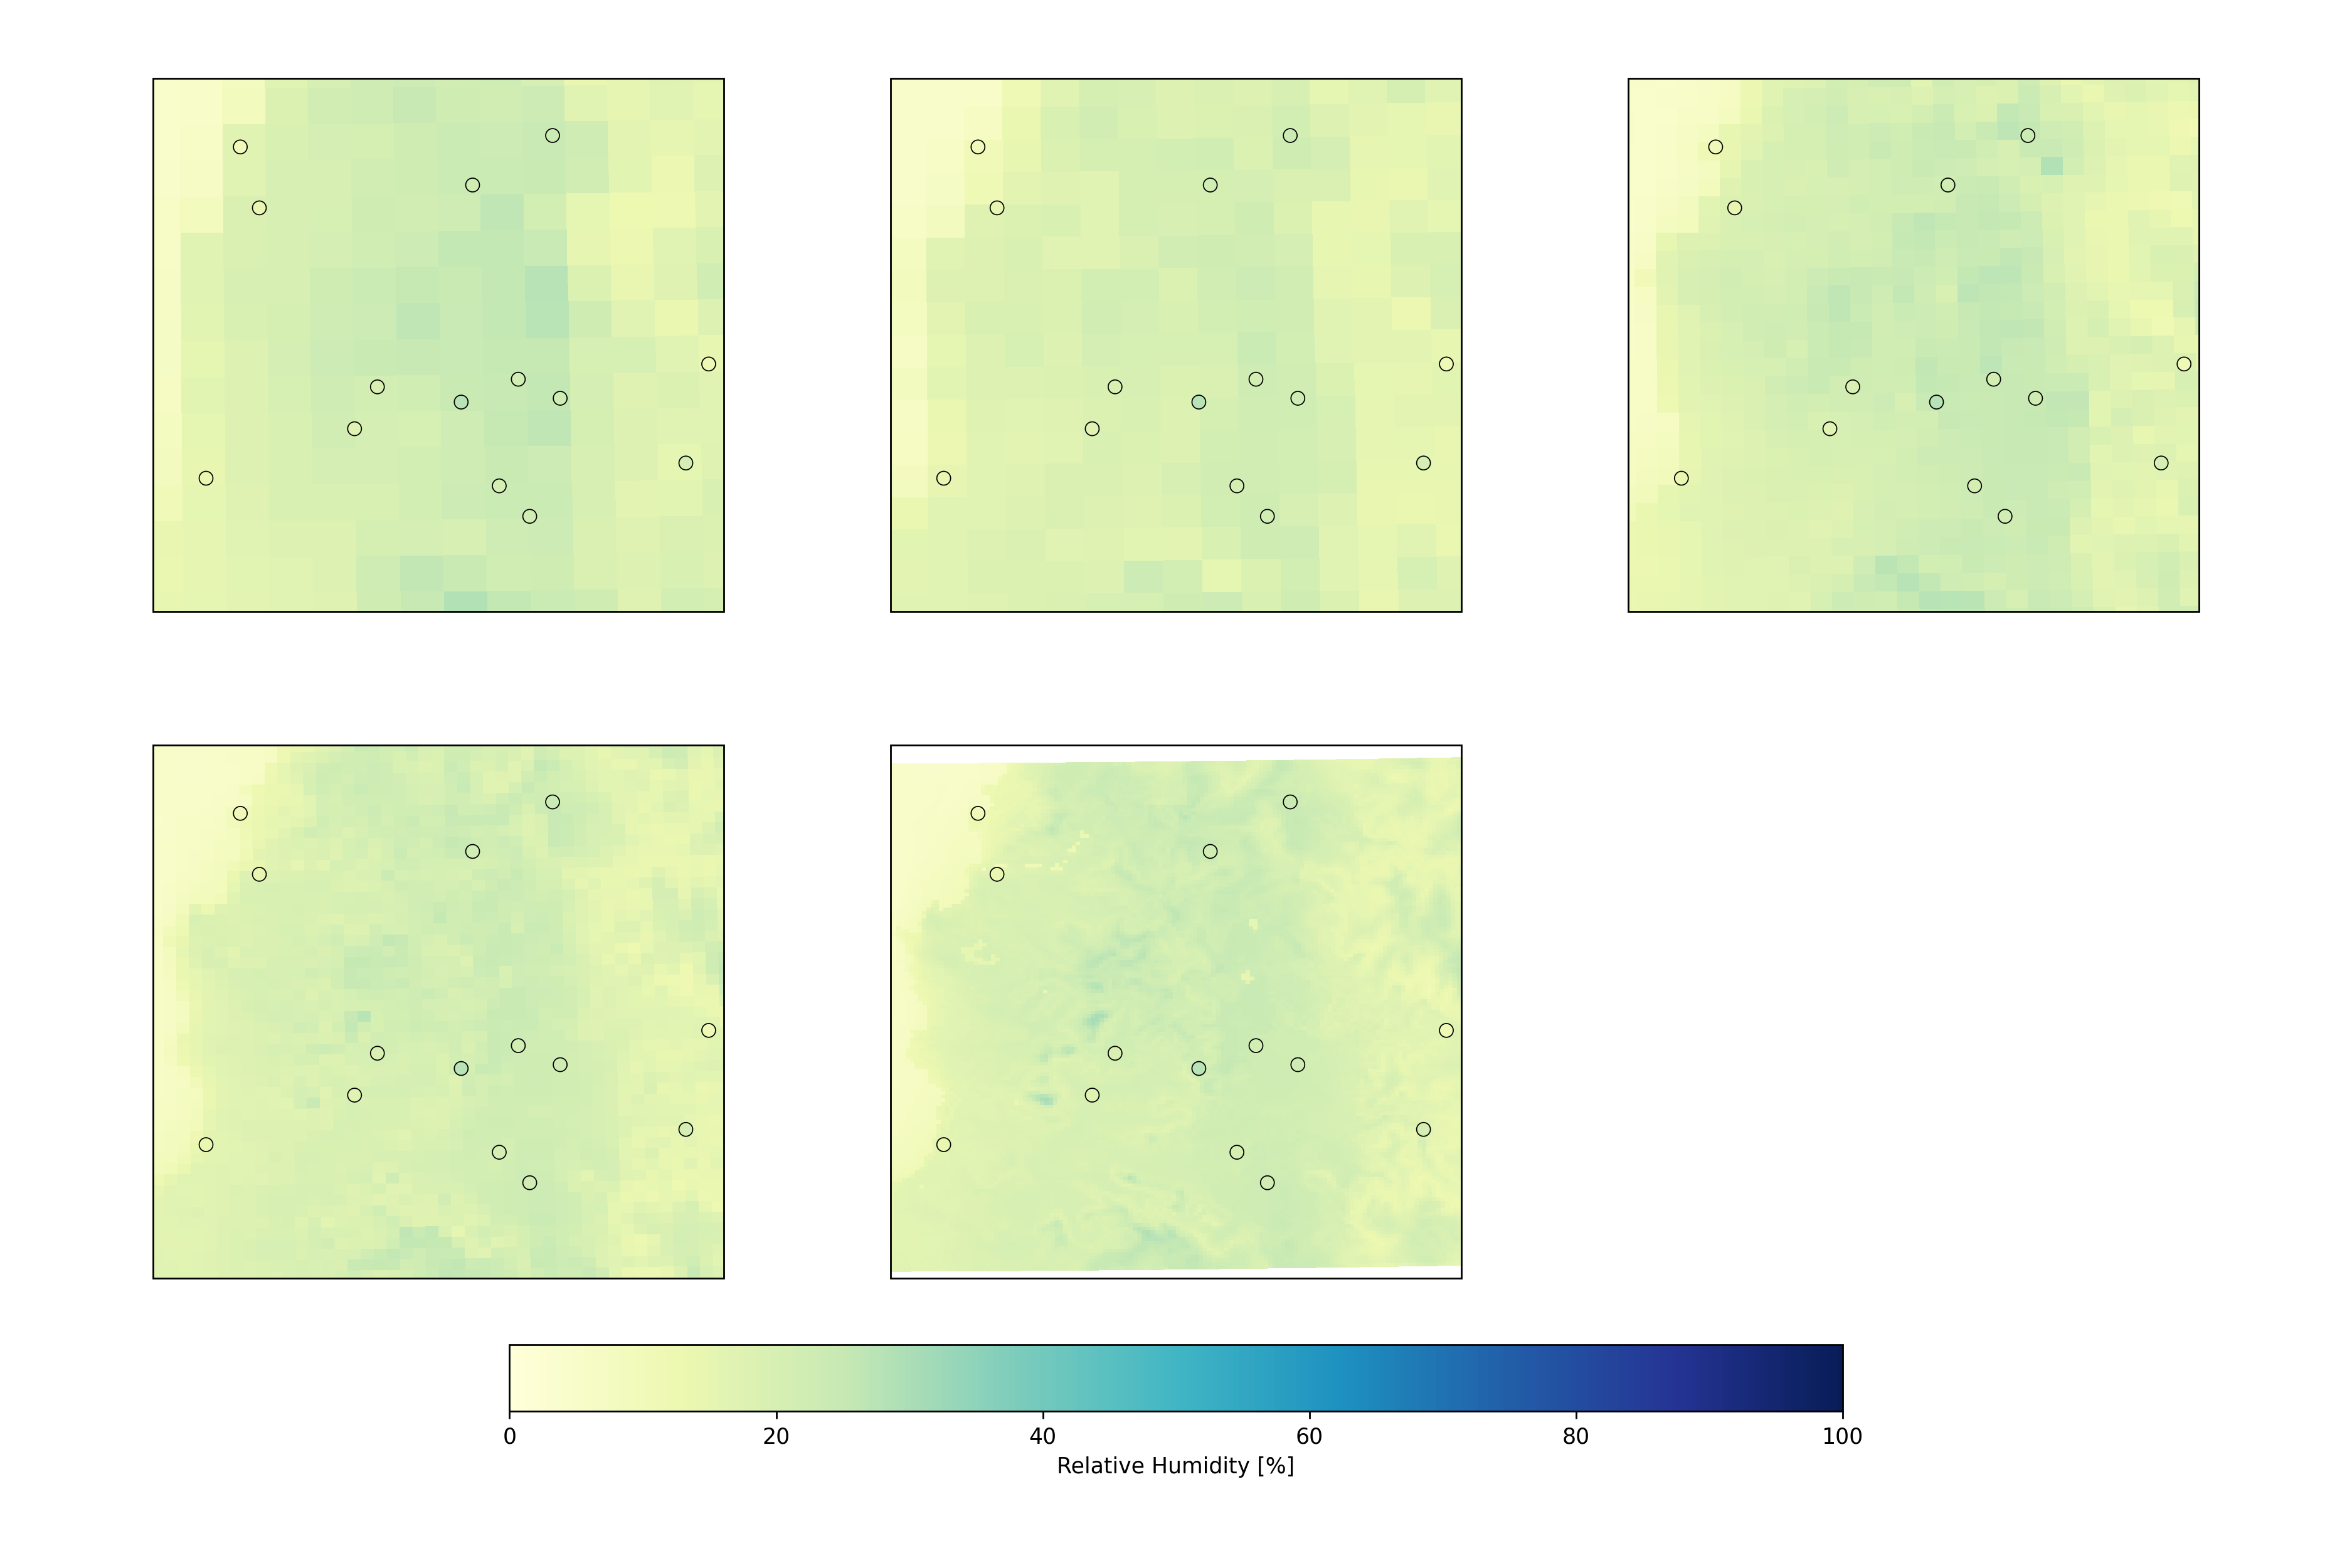
\includegraphics[width=\linewidth,height=8cm]{Annex_3.i.png}
    \textbf{Annex 3.i} Temporal standard deviation of configuration C for 2-meter relative humidity fields across Central Chile (colormap), compared to the temporal standard deviation of the station observations for the same period (scatterplots).  The corresponding leadtime is of 24 hours
\end{figure}

\begin{figure}[htbp]
    \centering
    \begin{minipage}{0.31\textwidth}
        \centering
        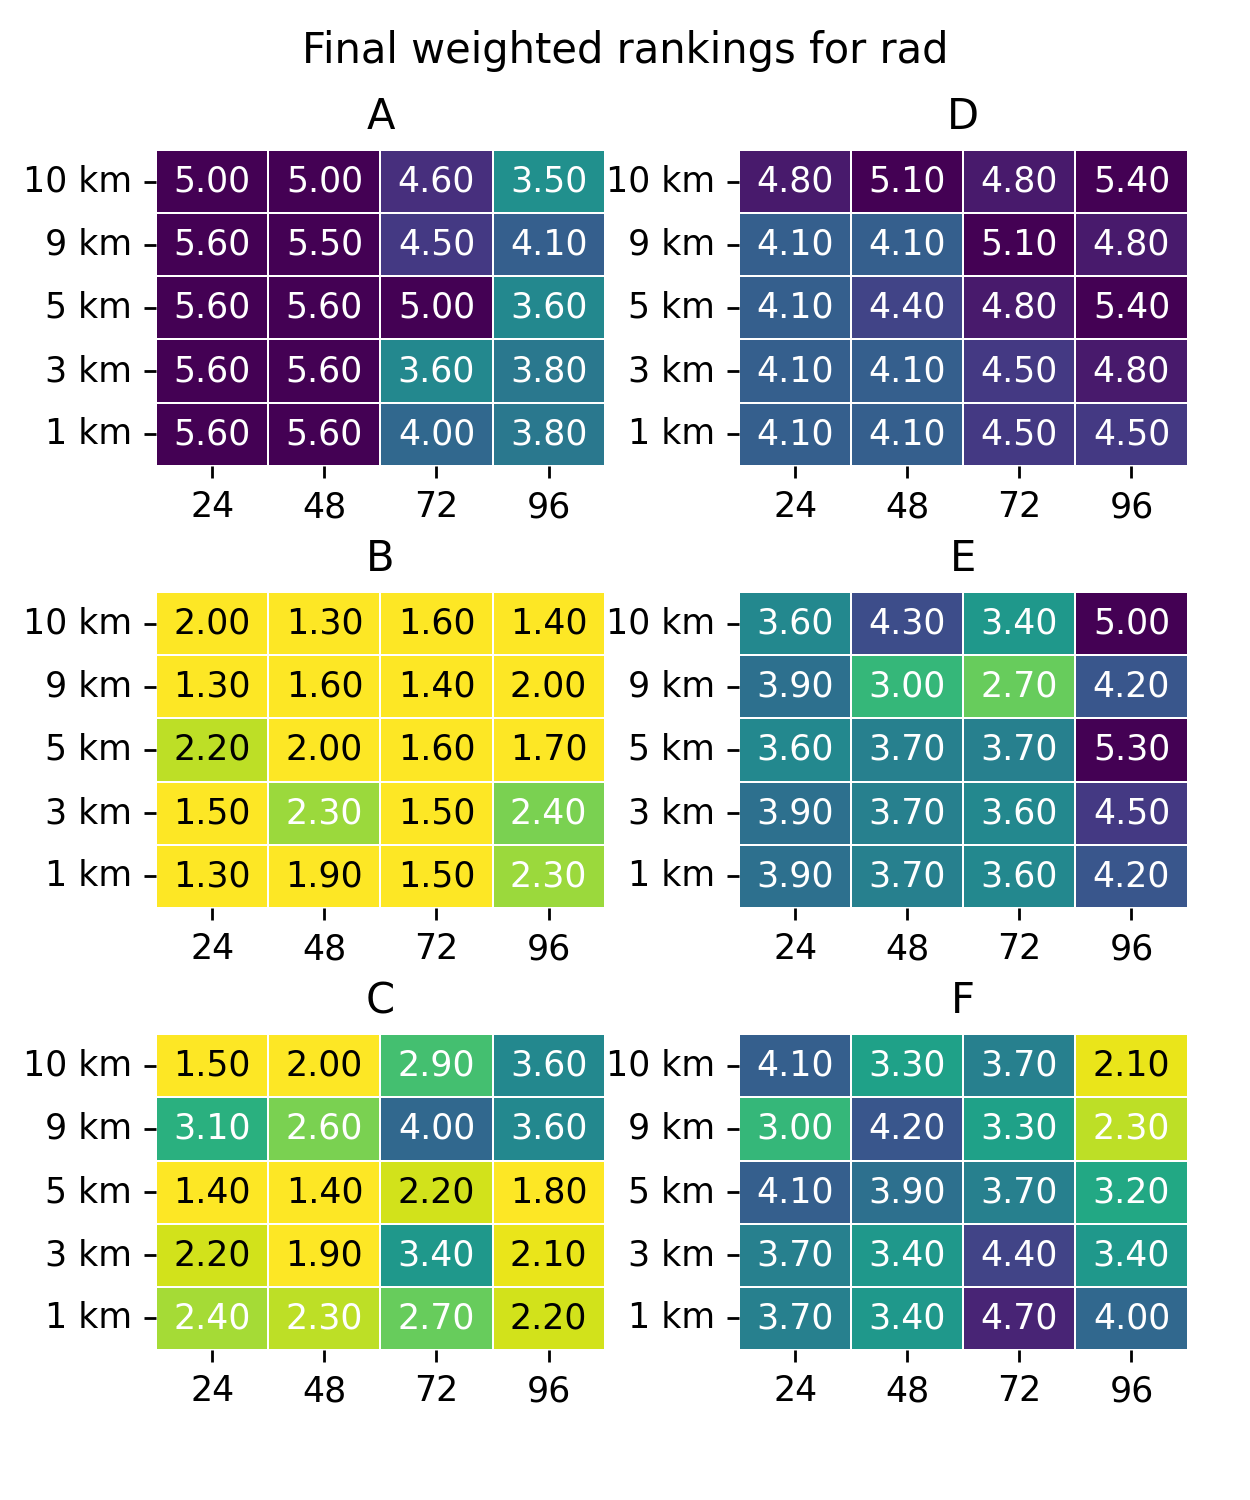
\includegraphics[width=\linewidth]{Annex_4.a.png}
   
    \end{minipage}
    \hfill
    \begin{minipage}{0.31\textwidth}
        \centering
        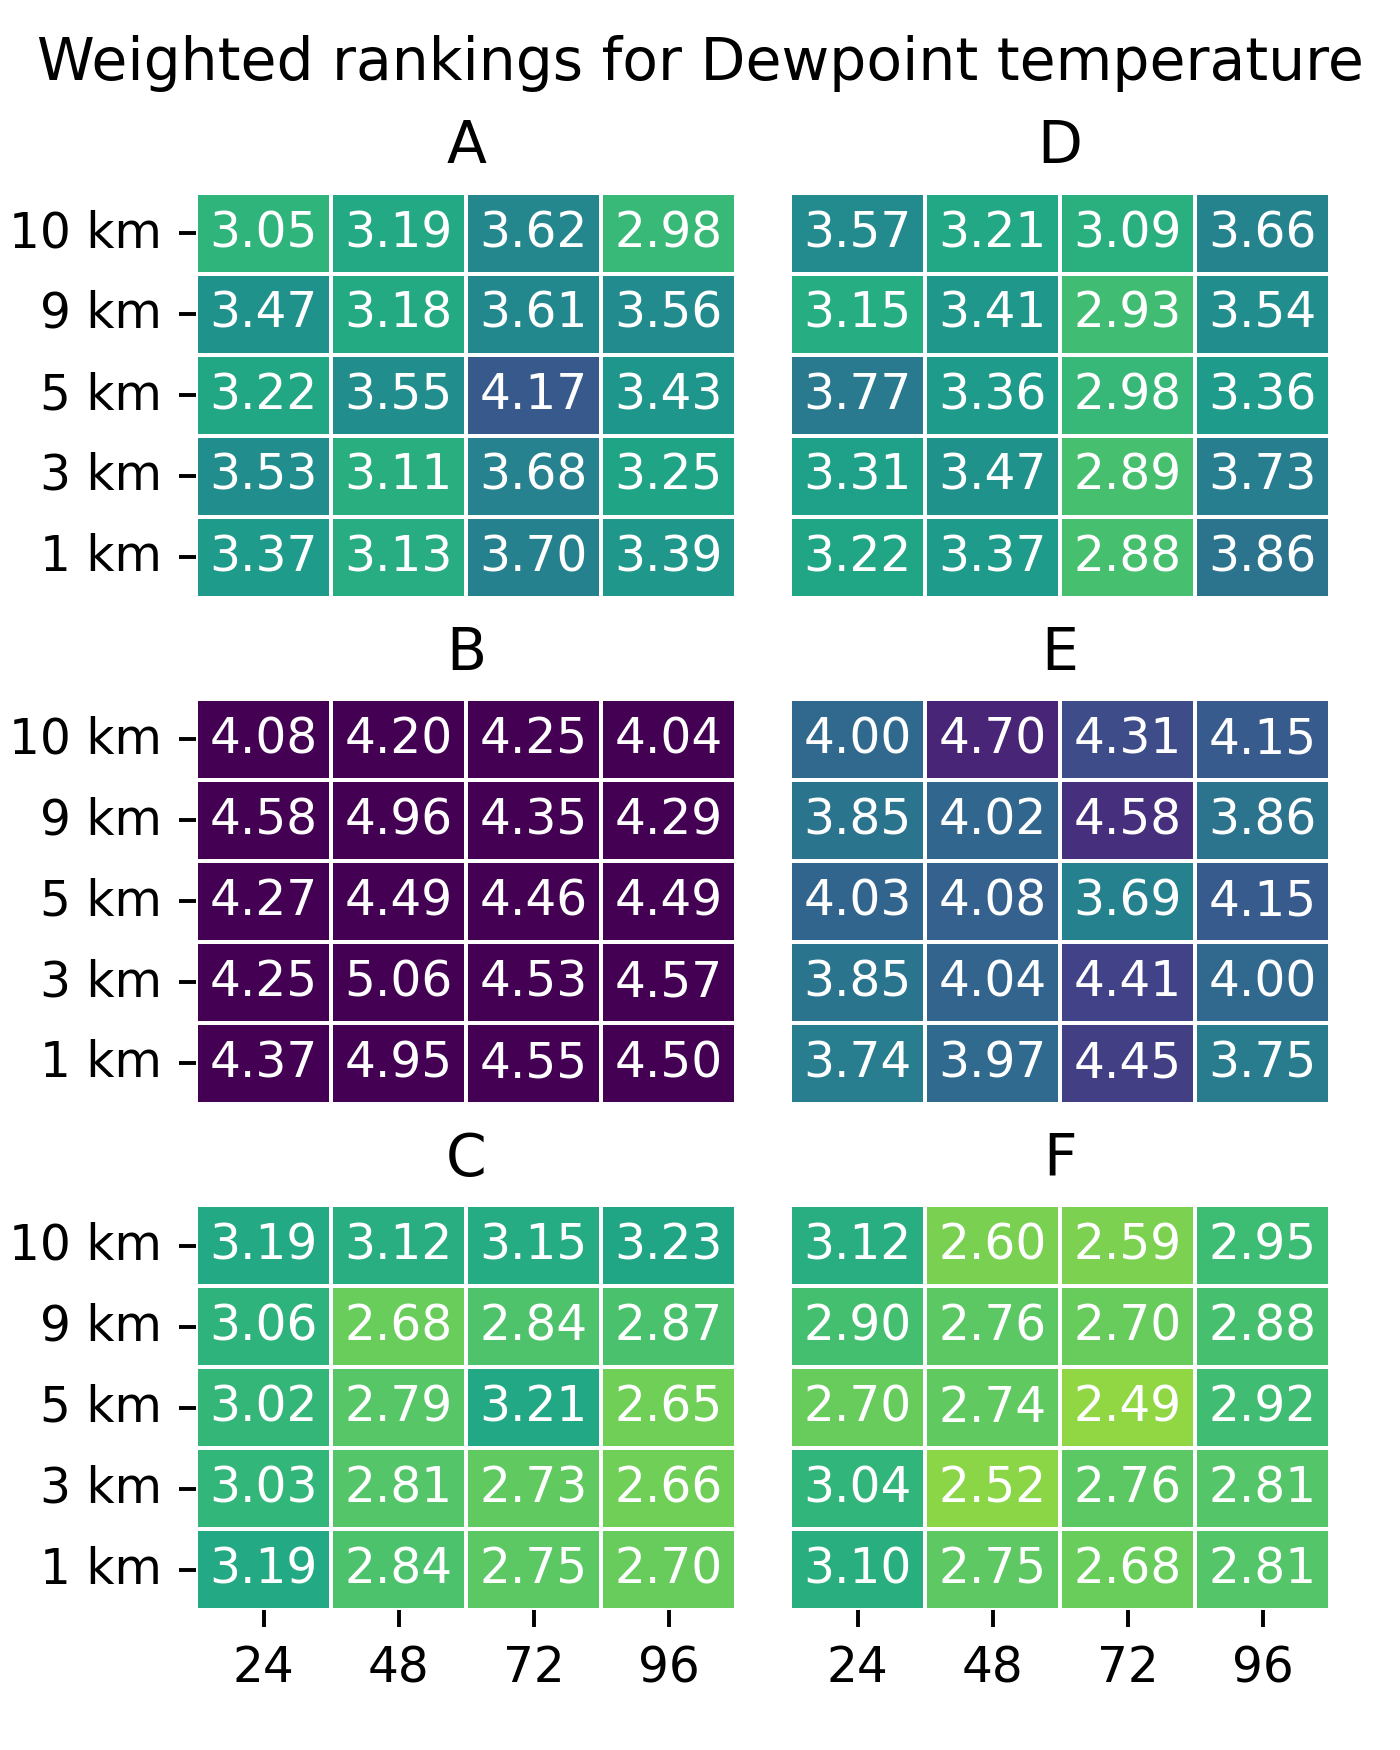
\includegraphics[width=\linewidth]{Annex_4.b.png}
  
    \end{minipage}
     \hfill
    \begin{minipage}{0.31\textwidth}
        \centering
        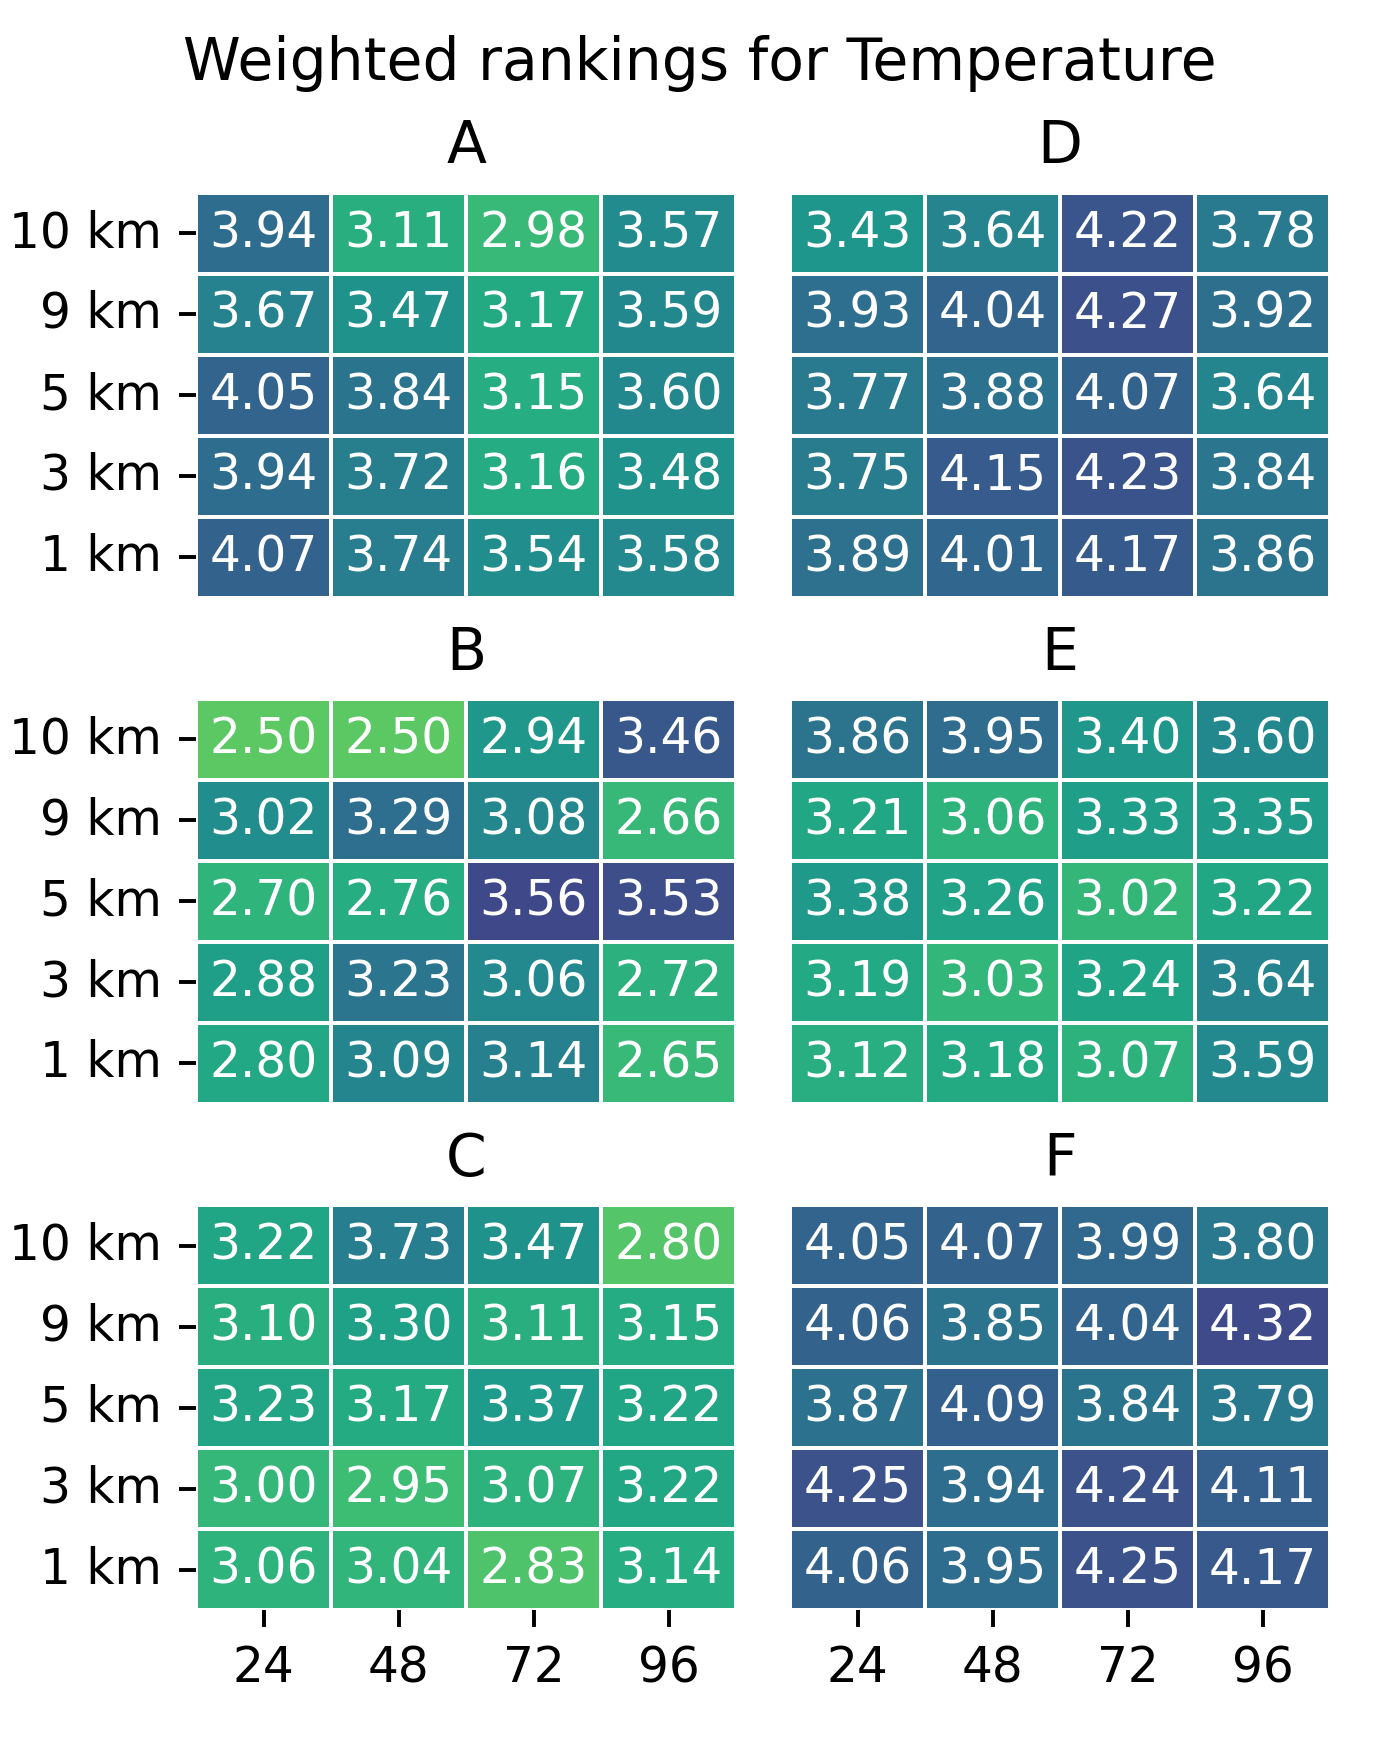
\includegraphics[width=\linewidth]{Annex_4.c.png}
    \end{minipage}
    \textbf{Annex 4} Statistical performance metrics used to evaluate WRF configurations for incoming shortwave solar radiation (left) dewpoint (center) and temperature (right). Lower score indicates overall better performance relative to other ranked configurations for the same resolution and leadtime corresponding to each cell.
\end{figure}

\begin{figure}[htbp]
	\centering
	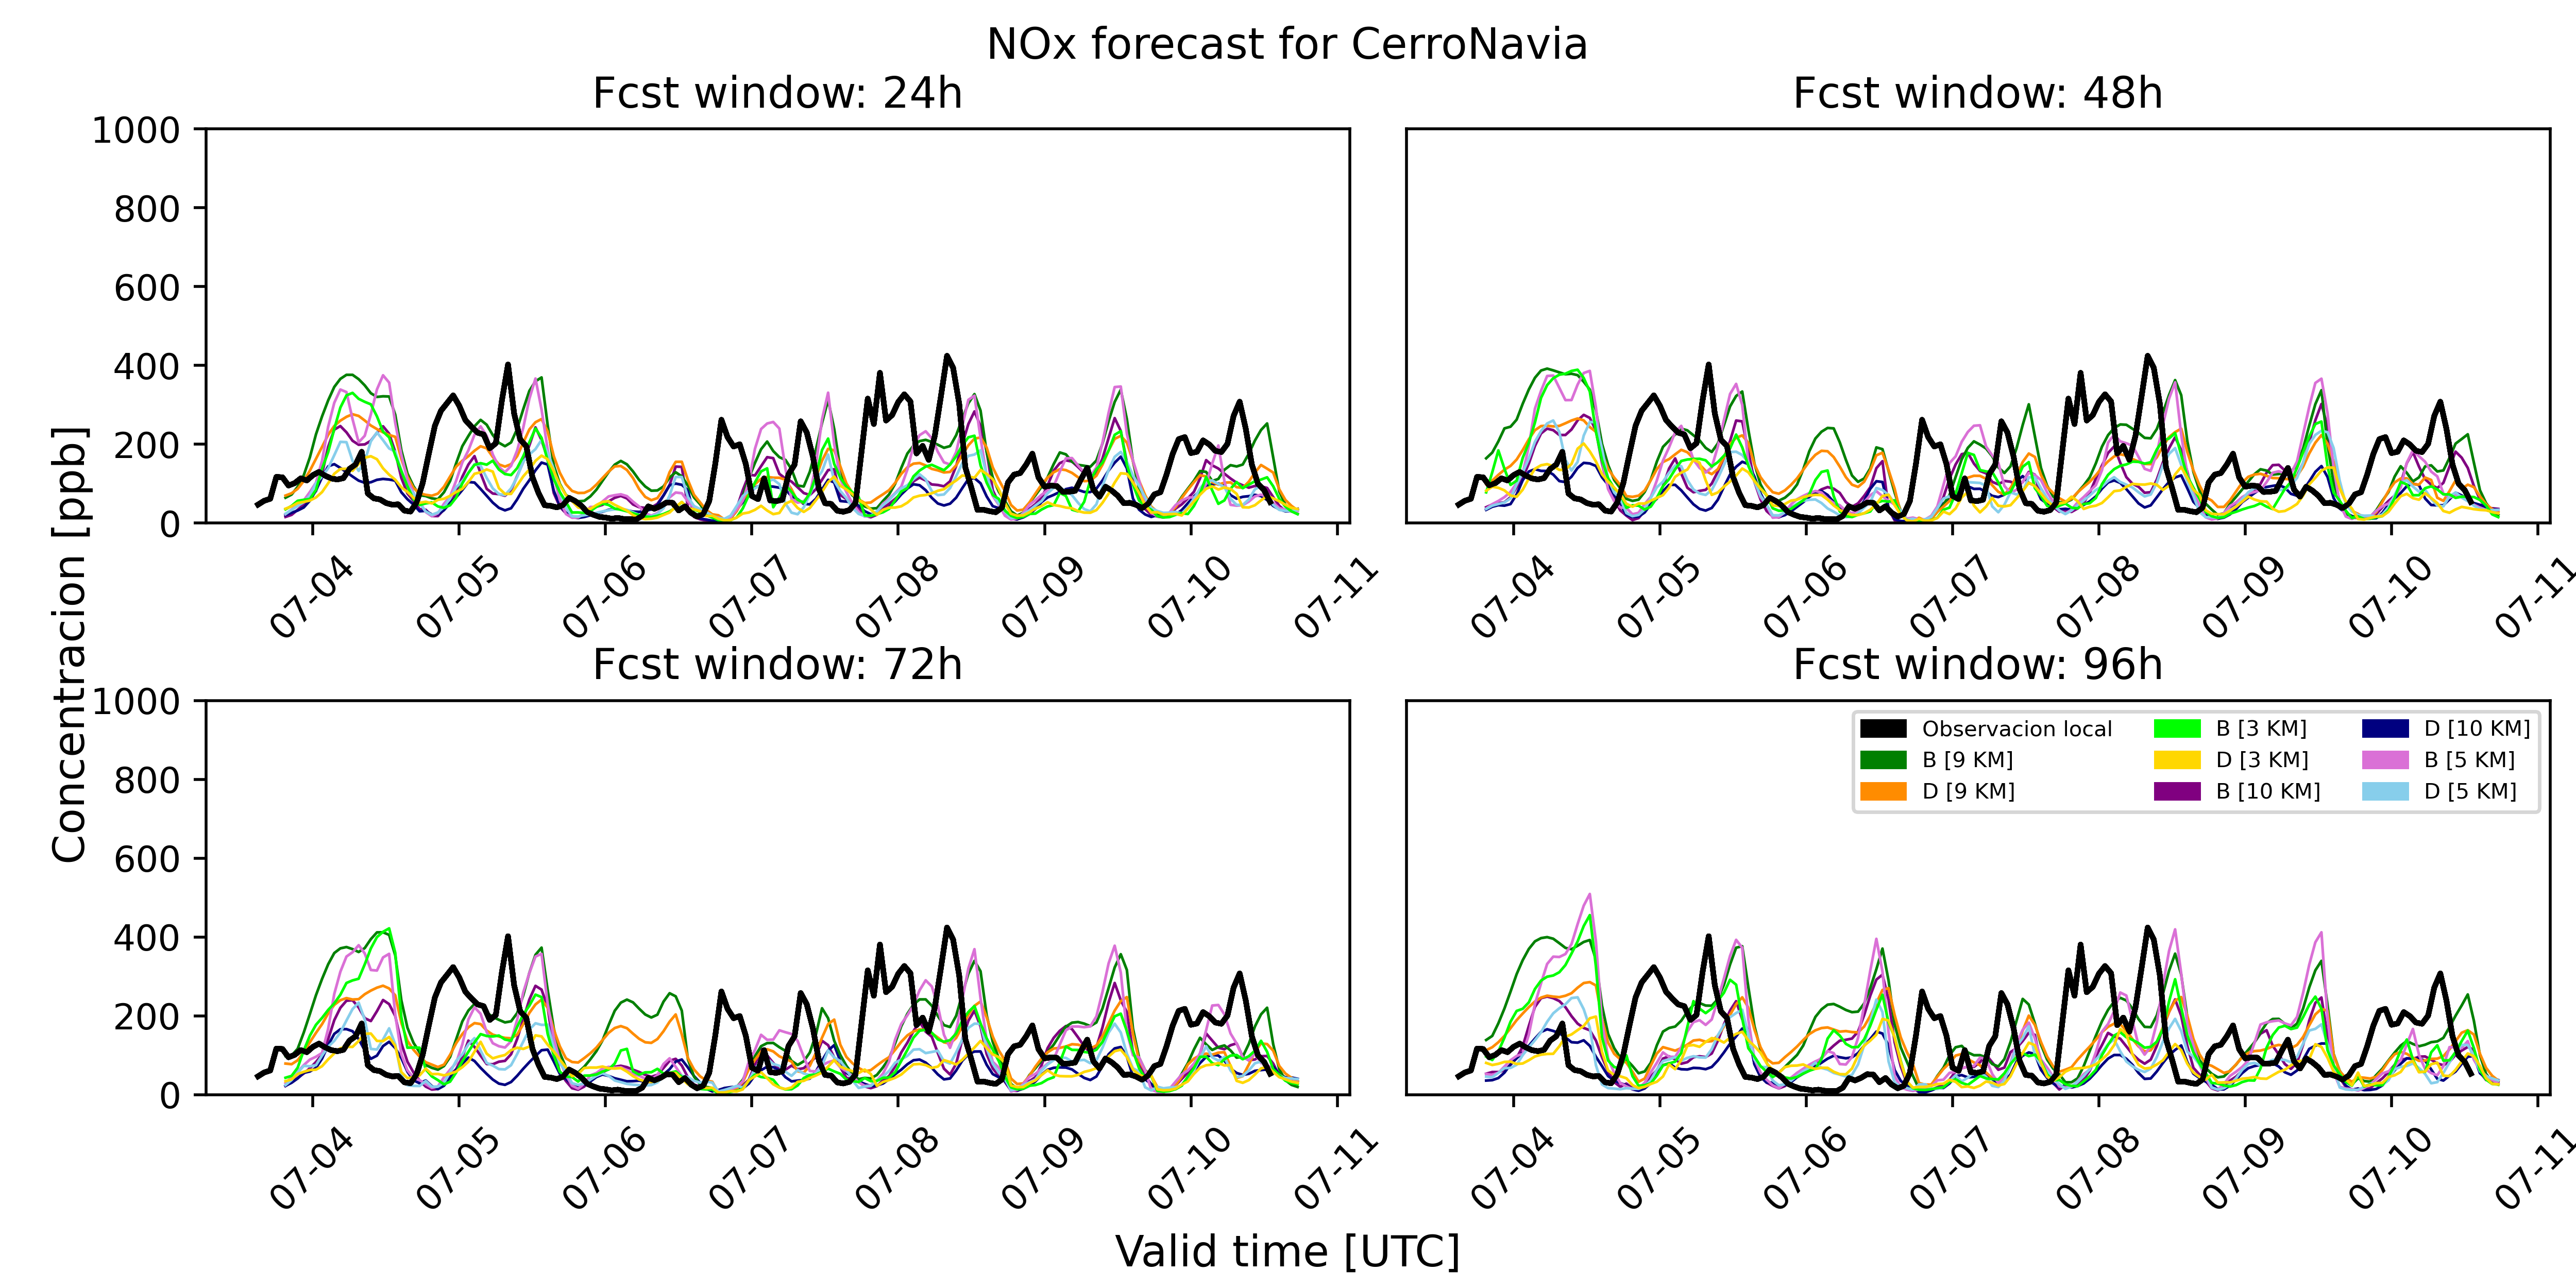
\includegraphics[width=0.99\textwidth]{Annex_5.a.png}
	\textbf{Annex 5.a} Forecast time series of NOx concentrations from the coupled WRF-CHIMERE system at the Cerro Navia SINCA station. Each subplot represents a leadtime (labeled in the subplot's title), showing observed (black) and forecasted time series (colors by configuration/resolution). These forecasts are simulated from the INEMA emission inventory.
	\label{fig:figure5}
\end{figure}

\begin{figure}[htbp]
	\centering
	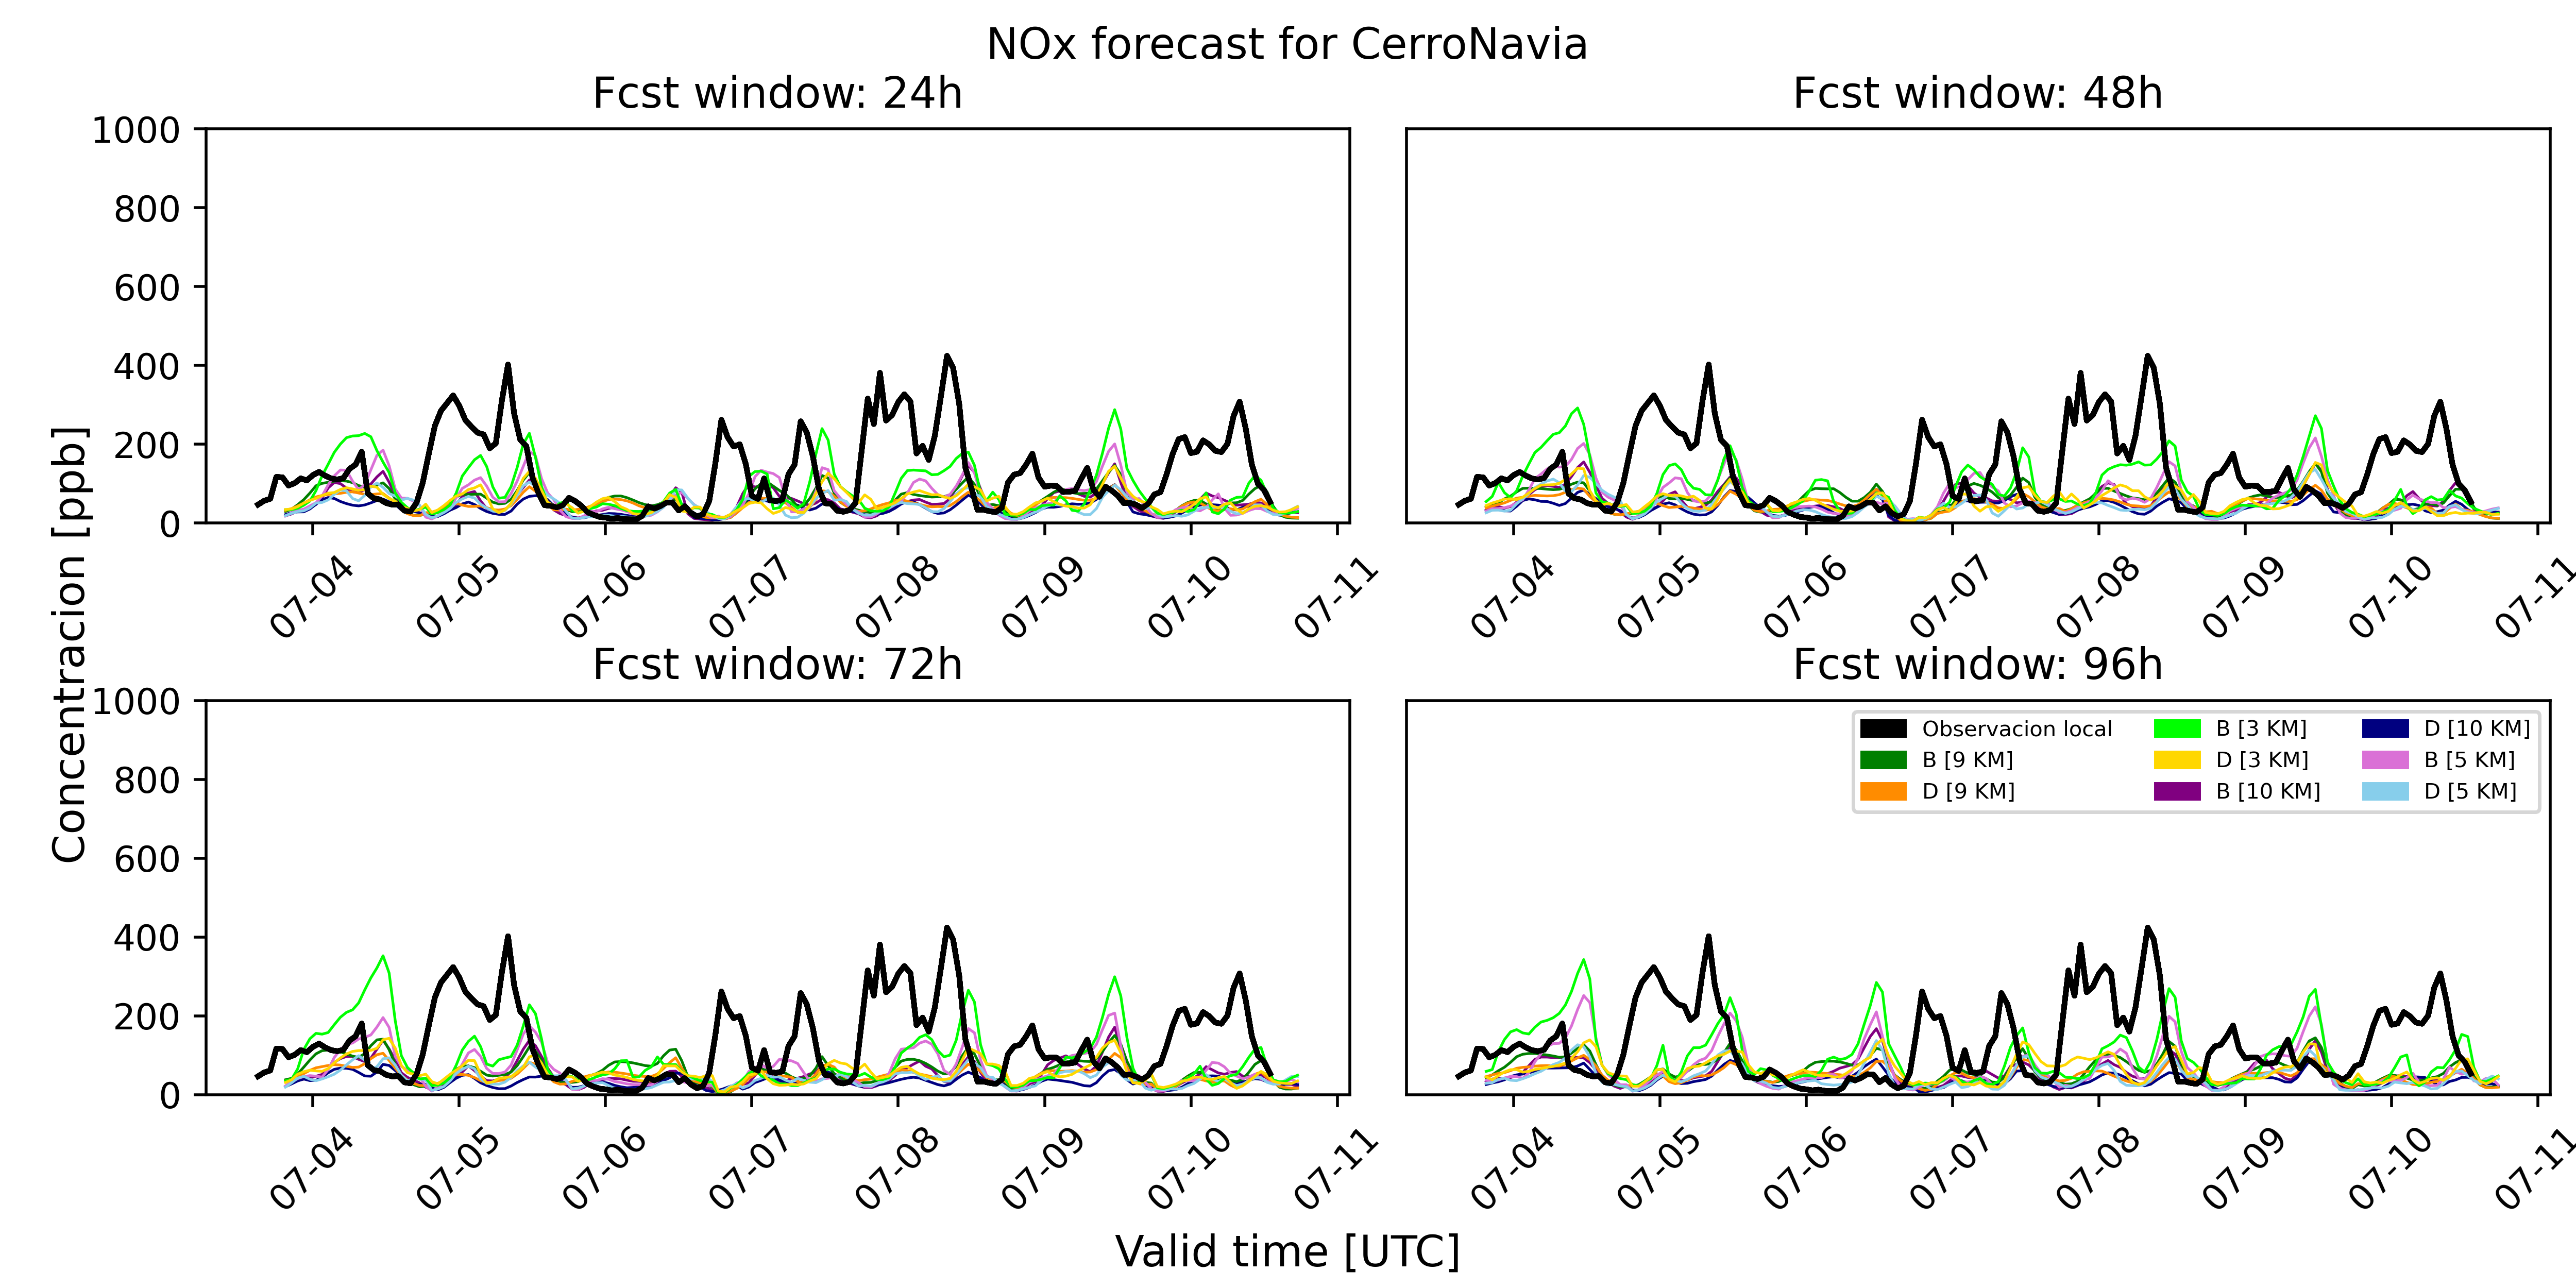
\includegraphics[width=0.99\textwidth]{Annex_5.b.png}
	\textbf{Annex 5.b} Forecast time series of NOx concentrations from the coupled WRF-CHIMERE system at the Cerro Navia SINCA station. Each subplot represents a leadtime (labeled in the subplot's title), showing observed (black) and forecasted time series (colors by configuration/resolution). These forecasts are simulated from the CAMS emission inventory.
	\label{fig:figure5}
\end{figure}

\begin{figure}[htbp]
    \centering
    \begin{minipage}{0.49\textwidth}
        \centering
        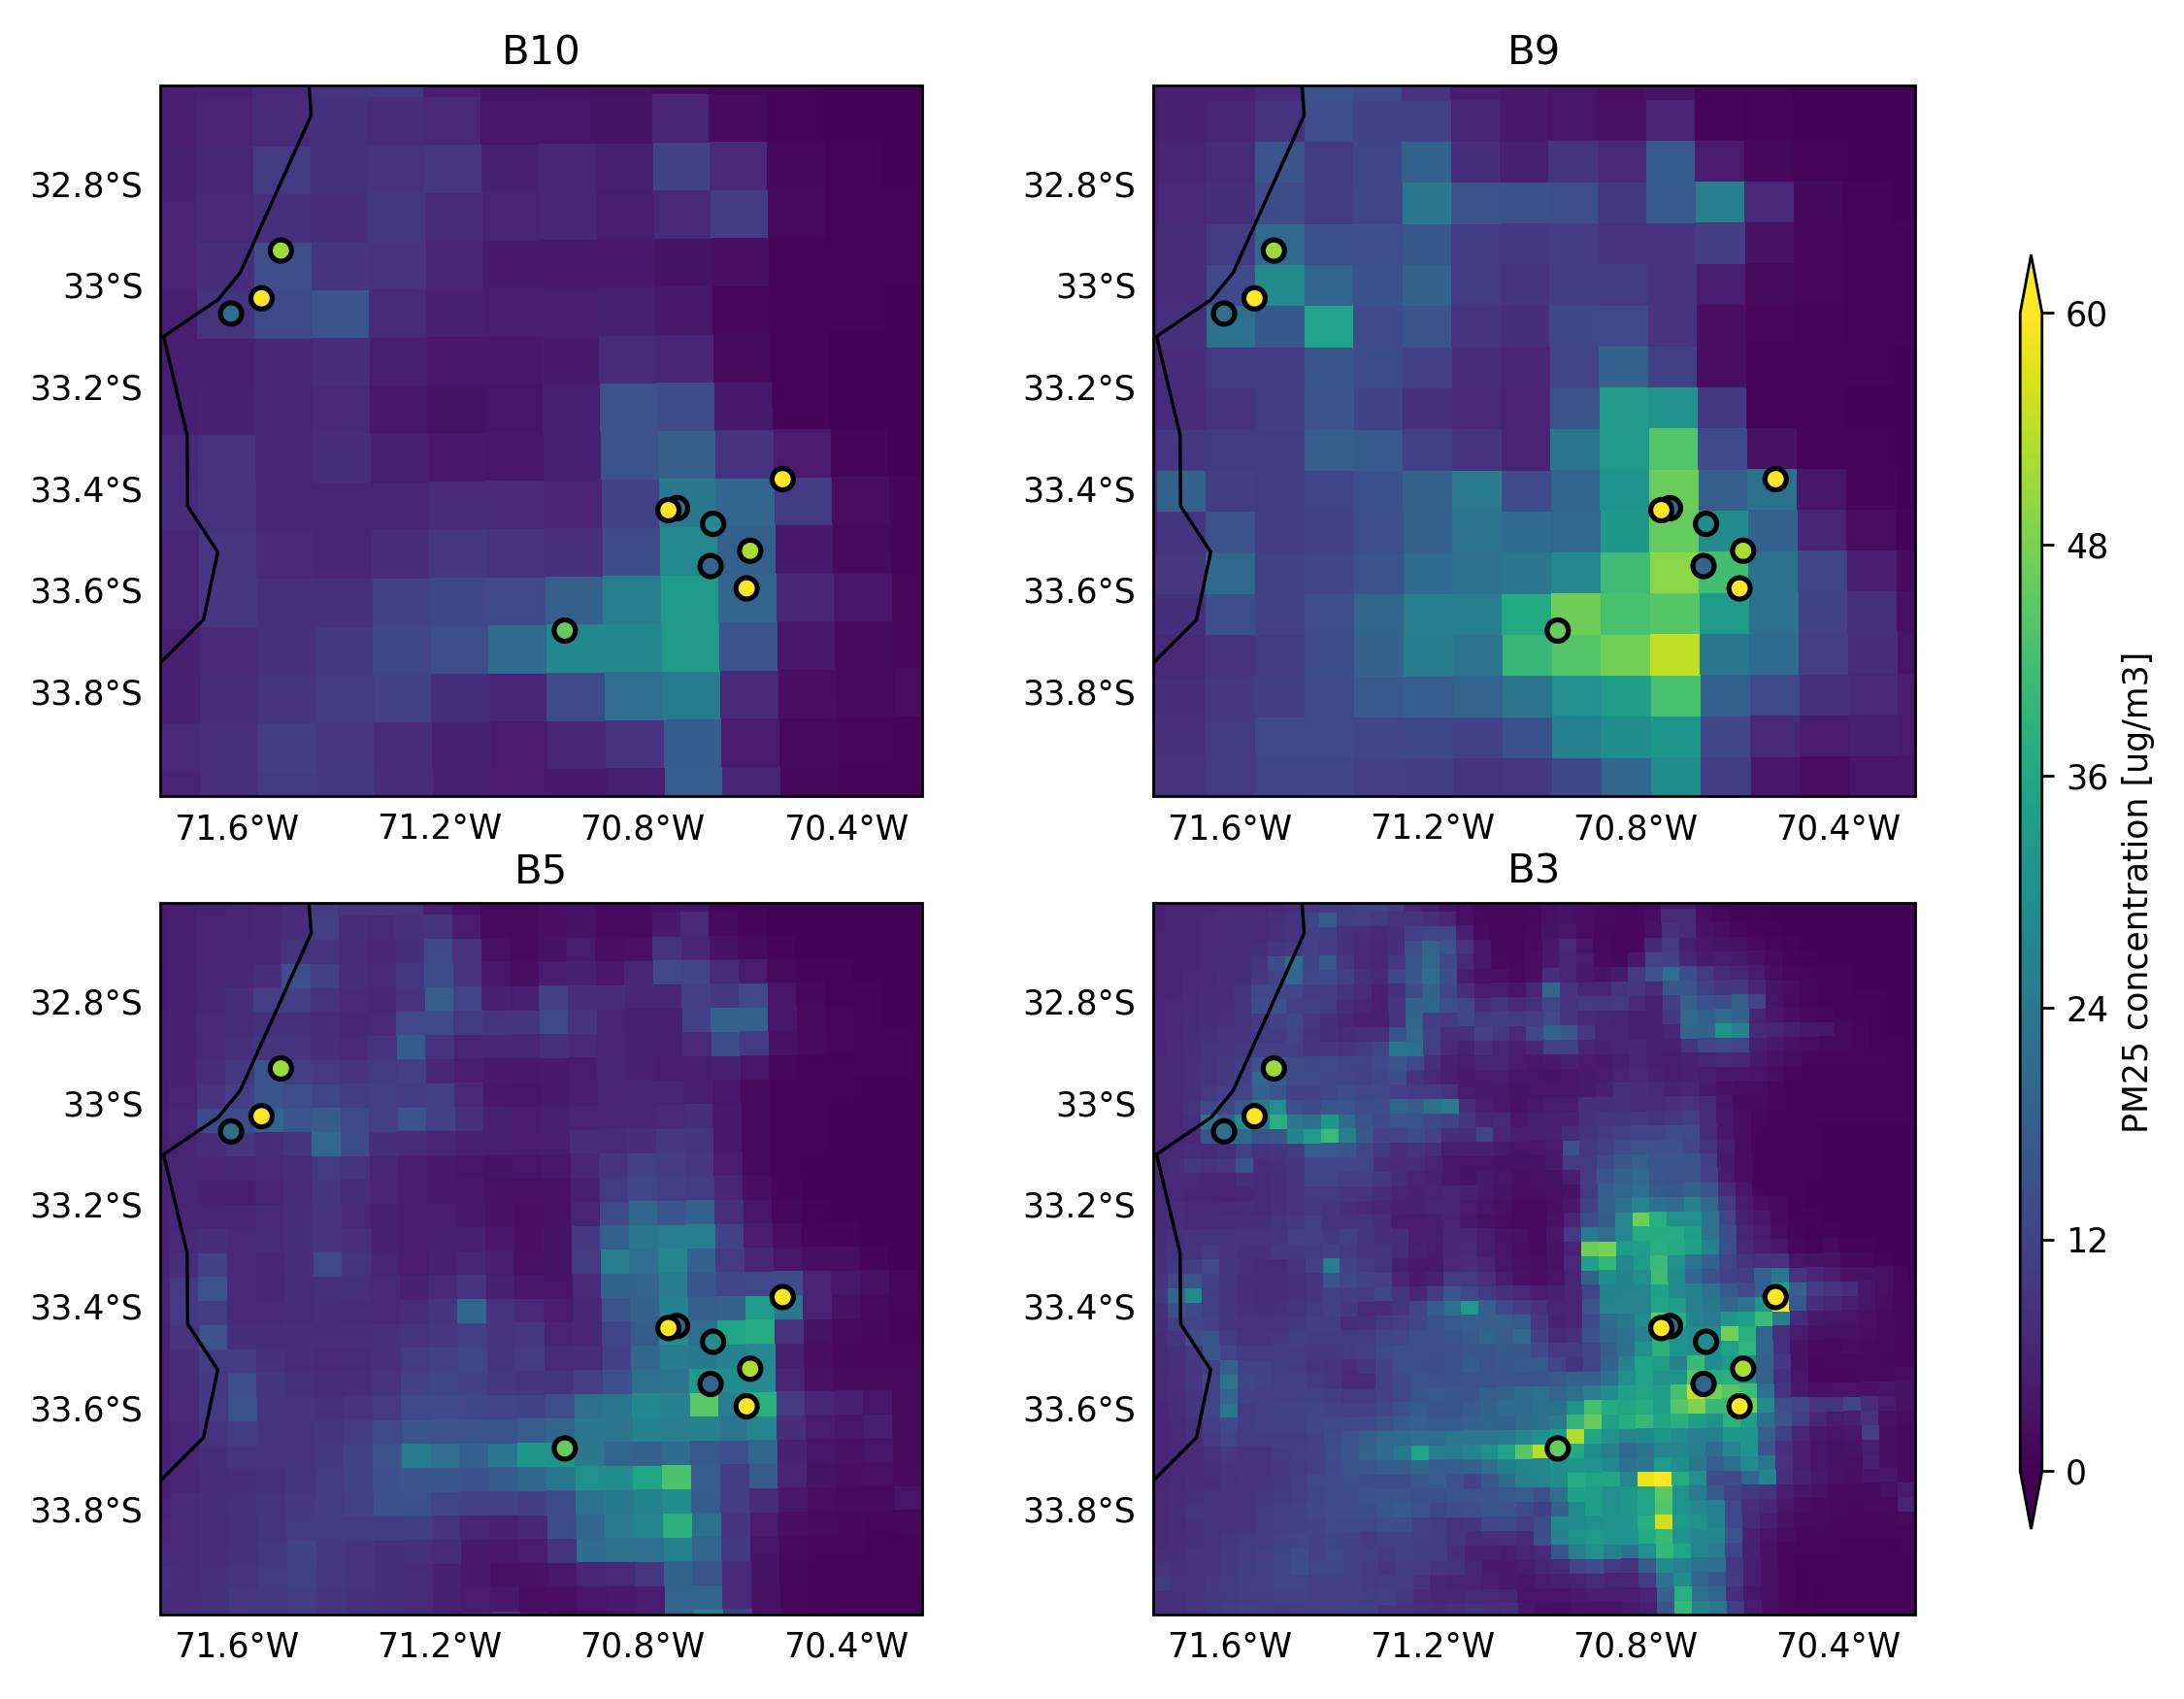
\includegraphics[width=\linewidth]{Annex_6.a.png}
    \end{minipage}
    \hfill
    \begin{minipage}{0.49\textwidth}
        \centering
        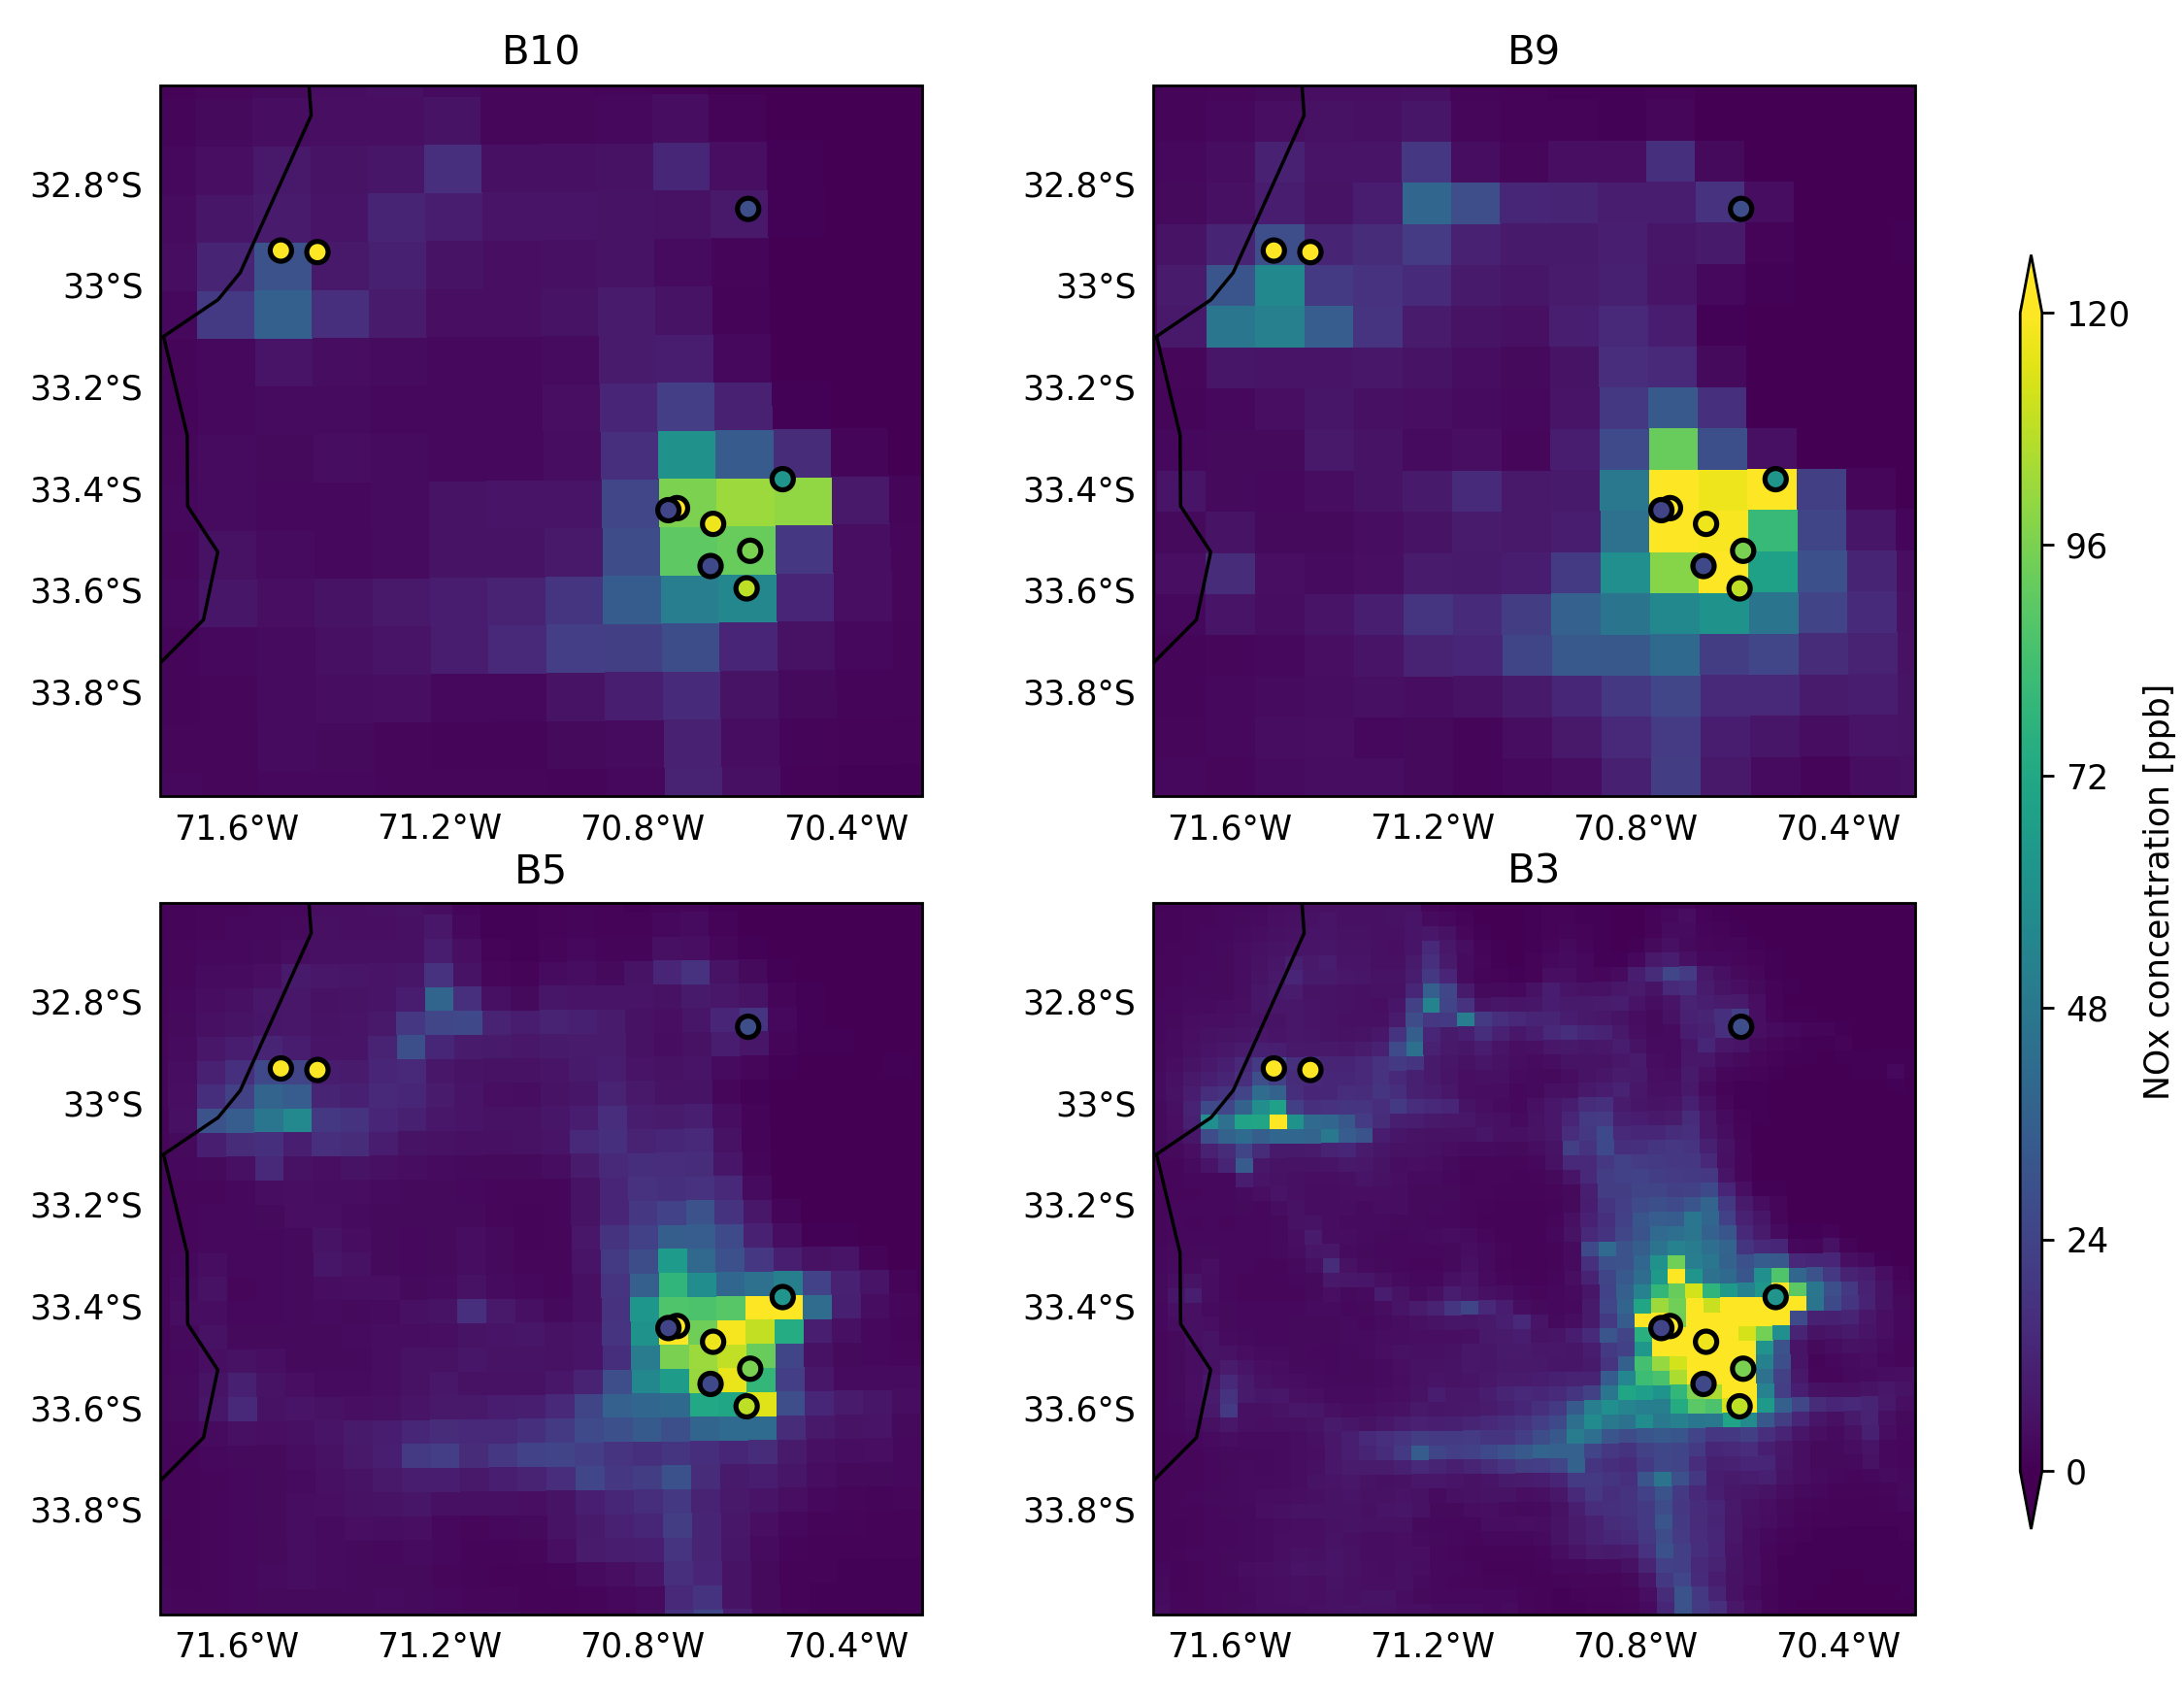
\includegraphics[width=\linewidth]{Annex_6.b.png}
    \end{minipage}
    \textbf{Annex 6} Temporal mean of PM25 (left) and NOx (right) concentrations from the coupled WRF--CHIMERE system, compared to SINCA stations (scatter plots). These fields were derived from the D WRF configuration and the INEMA emission inventory.
\end{figure}

\section{Bibliography}
\label{bibliography}
\begin{enumerate}
\def\labelenumi{\arabic{enumi}.}
\tightlist
\item
  Lapere, R., Menut, L., Mailler, S., \& Huneeus, N. (2021). Seasonal
  variation in atmospheric pollutants transport in central Chile:
  Dynamics and consequences. \emph{Atmospheric Chemistry and Physics,
  21}(8), 6431--6454. https://doi.org/10.5194/acp-21-6431-2021\\
\item
  Saide, P. E., Mena-Carrasco, M., Tolvett, S., Hernandez, P., \&
  Carmichael, G. R. (2016). Air quality forecasting for winter-time
  PM2.5 episodes occurring in multiple cities in central and southern
  Chile. \emph{Journal of Geophysical Research: Atmospheres, 121}(1),
  558--575. https://doi.org/10.1002/2015JD023949\\
\item
  Gao, C., Zhang, X., Xiu, A., Tong, Q., Zhao, H., Zhang, S., Yang, G.,
  Zhang, M., \& Xie, S. (2024). Intercomparison of multiple two-way
  coupled meteorology and air quality models (WRF v4.1.1--CMAQ v5.3.1,
  WRF--Chem v4.1.1, and WRF v3.7.1--CHIMERE v2020r1) in eastern China.
  \emph{Geoscientific Model Development, 17}(6), 2471--2492.
  https://doi.org/10.5194/gmd-17-2471-2024
\item 
  https://www.sciencedirect.com/science/article/pii/S0269749123007613
\item 
  https://agupubs.onlinelibrary.wiley.com/doi/full/10.1002/jgrd.50293?utm
\item 
  https://www.mdpi.com/2073-4433/15/1/10?utm
\end{enumerate}

\end{document}
